% !TeX encoding = UTF-8

% 载入 SJTUThesis 模版
\documentclass[type=bachelor]{sjtuthesis}
% 选项
%   type=[doctor|master|bachelor|course],     % 可选(默认:doctor),论文类型
%   zihao=[-4|5],                             % 可选(研究生默认:-4,本科默认:5),正文字号大小
%   lang=[zh|en],                             % 可选(默认:zh),论文的主要语言
%   review,                                   % 可选(默认:关闭),盲审模式
%   [twoside|oneside]                         % 可选(默认:twoside),单双页模式

% 论文基本配置,加载宏包等全局配置
\usepackage{pifont}
\usepackage{diagbox}
% !TEX root = ./main.tex

\sjtusetup{
  %
  %******************************
  % 注意:
  %   1. 配置里面不要出现空行
  %   2. 不需要的配置信息可以删除
  %******************************
  %
  % 信息录入
  %
  info = {%
    %
    % 标题
    %
    title           = {TPL-V Detector},
    title*          = {},
    %
    % 标题页标题
    %   可使用“\\”命令手动控制换行
    %
    % display-title   = {上海交通大学学位论文\\ \LaTeX{} 模板示例文档},
    % display-title*  = {A Sample Document \\ for \LaTeX-based SJTU Thesis Template},
    %
    % 页眉标题
    %
    % running-title   = {示例文档},
    % running-title*  = {Sample Document},
    %
    % 关键词
    %
    keywords        = {上海交大, 饮水思源, 爱国荣校},
    keywords*       = {SJTU, master thesis, XeTeX/LaTeX template},
    %
    % 姓名
    %
    author          = {某\quad{}某},
    author*         = {Mo Mo},
    %
    % 指导教师
    %
    supervisor      = {某某教授},
    supervisor*     = {Prof. Mou Mou},
    %
    % 副指导教师
    %
    % assisupervisor  = {某某教授},
    % assisupervisor* = {Prof. Uom Uom},
    %
    % 学号
    %
    id              = {0010900990},
    %
    % 学位
    %   本科生不需要填写
    %
    degree          = {工学硕士},
    degree*         = {Master of Engineering},
    %
    % 专业
    %
    major           = {某某专业},
    major*          = {A Very Important Major},
    %
    % 所属院系
    %
    department      = {某某系},
    department*     = {Depart of XXX},
    %
    % 课程名称
    %   仅课程论文适用
    %
    course          = {某某课程},
    %
    % 答辩日期
    %   使用 ISO 格式 (yyyy-mm-dd);默认为当前时间
    %
    % date            = {2014-12-17},
    %
    % 资助基金
    %
    % fund  = {
    %           {国家 973 项目 (No. 2025CB000000)},
    %           {国家自然科学基金 (No. 81120250000)},
    %         },
    % fund* = {
    %           {National Basic Research Program of China (Grant No. 2025CB000000)},
    %           {National Natural Science Foundation of China (Grant No. 81120250000)},
    %         },
  },
  %
  % 风格设置
  %
  style = {%
    %
    % 本科论文页眉 logo 颜色 (red/blue/black)
    %
    % header-logo-color = black,
  },
  %
  % 名称设置
  %
  name = {
    % bib               = {References},
    % acknowledgements  = {谢\hspace{\ccwd}辞},
    % publications      = {攻读学位期间完成的论文},
  },
}

% 使用 BibLaTeX 处理参考文献
%   biblatex-gb7714-2015 常用选项
%     gbnamefmt=lowercase     姓名大小写由输入信息确定
%     gbpub=false             禁用出版信息缺失处理
\usepackage[backend=biber,style=gb7714-2015]{biblatex}
% 文献表字体
% \renewcommand{\bibfont}{\zihao{-5}}
% 文献表条目间的间距
\setlength{\bibitemsep}{0pt}
% 导入参考文献数据库
\addbibresource{bibdata/thesis.bib}

% 定义图片文件目录与扩展名
\graphicspath{{figures/}}
\DeclareGraphicsExtensions{.pdf,.eps,.png,.jpg,.jpeg}

% 确定浮动对象的位置,可以使用 [H],强制将浮动对象放到这里(可能效果很差)
% \usepackage{float}

% 固定宽度的表格
% \usepackage{tabularx}

% 使用三线表:toprule,midrule,bottomrule。
\usepackage{booktabs}

% 表格中支持跨行
\usepackage{multirow}

% 表格中数字按小数点对齐
\usepackage{dcolumn}
\newcolumntype{d}[1]{D{.}{.}{#1}}

% 使用长表格
\usepackage{longtable}

% 附带脚注的表格
\usepackage{threeparttable}

% 附带脚注的长表格
\usepackage{threeparttablex}

% 算法环境宏包
\usepackage[ruled,vlined,linesnumbered]{algorithm2e}
% \usepackage{algorithm, algorithmicx, algpseudocode}

% 代码环境宏包
\usepackage{listings}
\lstnewenvironment{codeblock}[1][]%
  {\lstset{style=lstStyleCode,#1}}{}

% 物理科学和技术中使用的数学符号,定义了 \qty 命令,与 siunitx 3.0 有冲突
% \usepackage{physics}

% 直立体数学符号
\newcommand{\dd}{\mathop{}\!\mathrm{d}}
\newcommand{\ee}{\mathrm{e}}
\newcommand{\ii}{\mathrm{i}}
\newcommand{\jj}{\mathrm{j}}

% 国际单位制宏包
\usepackage{siunitx}[=v2]

% 定理环境宏包
\usepackage{ntheorem}
% \usepackage{amsthm}

% 绘图宏包
\usepackage{tikz}
\usetikzlibrary{shapes.geometric, arrows}

% 一些文档中用到的 logo
\usepackage{hologo}
\newcommand{\XeTeX}{\hologo{XeTeX}}
\newcommand{\BibLaTeX}{\textsc{Bib}\LaTeX}

% 借用 ltxdoc 里面的几个命令方便写文档
\DeclareRobustCommand\cs[1]{\texttt{\char`\\#1}}
\providecommand\pkg[1]{{\sffamily#1}}

% 自定义命令

% E-mail
\newcommand{\email}[1]{\href{mailto:#1}{\texttt{#1}}}

% hyperref 宏包在最后调用
\usepackage{hyperref}

% 自动引用题注更正为中文
\def\equationautorefname{式}
\def\footnoteautorefname{脚注}
\def\itemautorefname{项}
\def\figureautorefname{图}
\def\tableautorefname{表}
\def\partautorefname{篇}
\def\appendixautorefname{附录}
\def\chapterautorefname{章}
\def\sectionautorefname{节}
\def\subsectionautorefname{小节}
\def\subsubsectionautorefname{小节}
\def\paragraphautorefname{段落}
\def\subparagraphautorefname{子段落}
\def\FancyVerbLineautorefname{行}
\def\theoremautorefname{定理}


\begin{document}

%TC:ignore

% 标题页
\maketitle

% 原创性声明及使用授权书
\copyrightpage
% 插入外置原创性声明及使用授权书
% \copyrightpage[scans/sample-copyright-old.pdf]

% 前置部分
\frontmatter

% 摘要
% !TEX root = ../main.tex

\begin{abstract}
  中文摘要应该将学位论文的内容要点简短明了地表达出来,应该包含论文中的基本信息,
  体现科研工作的核心思想。摘要内容应涉及本项科研工作的目的和意义、研究方法、研究
  成果、结论及意义。注意突出学位论文中具有创新性的成果和新见解的部分。摘要中不宜
  使用公式、化学结构式、图表和非公知公用的符号和术语,不标注引用文献编号。硕士学
  位论文中文摘要字数为 500 字左右,博士学位论文中文摘要字数为 800 字左右。英文摘
  要内容应与中文摘要内容一致。

  摘要页的下方注明本文的关键词(4~6个)。
\end{abstract}

\begin{abstract*}
  Shanghai Jiao Tong University (SJTU) is a key university in China. SJTU was
  founded in 1896. It is one of the oldest universities in China. The University
  has nurtured large numbers of outstanding figures include JIANG Zemin, DING
  Guangen, QIAN Xuesen, Wu Wenjun, WANG An, etc.

  SJTU has beautiful campuses, Bao Zhaolong Library, Various laboratories. It
  has been actively involved in international academic exchange programs. It is
  the center of CERNet in east China region, through computer networks, SJTU has
  faster and closer connection with the world.
\end{abstract*}


% 目录
\tableofcontents
% 插图索引
%\listoffigures*
% 表格索引
%\listoftables*
% 算法索引
%\listofalgorithms*

% 符号对照表
%% !TEX root = ../main.tex

\begin{nomenclature*}
\label{chap:symb}

\begin{longtable}{rl}
  $\epsilon$  & 介电常数  \\  
  $\mu$       & 磁导率    \\
  $\epsilon$  & 介电常数  \\
  $\mu$       & 磁导率    \\
  $\epsilon$  & 介电常数  \\
  $\mu$       & 磁导率    \\
  $\epsilon$  & 介电常数  \\
  $\mu$       & 磁导率    \\
  $\epsilon$  & 介电常数  \\
  $\mu$       & 磁导率    \\
  $\epsilon$  & 介电常数  \\
  $\mu$       & 磁导率    \\
  $\epsilon$  & 介电常数  \\
  $\mu$       & 磁导率    \\
  $\epsilon$  & 介电常数  \\
  $\mu$       & 磁导率    \\
  $\epsilon$  & 介电常数  \\
  $\mu$       & 磁导率    \\
  $\epsilon$  & 介电常数  \\
  $\mu$       & 磁导率    \\
  $\epsilon$  & 介电常数  \\
  $\mu$       & 磁导率    \\
  $\epsilon$  & 介电常数  \\
  $\mu$       & 磁导率    \\
  $\epsilon$  & 介电常数  \\
  $\mu$       & 磁导率    \\
  $\epsilon$  & 介电常数  \\
  $\mu$       & 磁导率    \\
  $\epsilon$  & 介电常数  \\
  $\mu$       & 磁导率    \\
  $\epsilon$  & 介电常数  \\
  $\mu$       & 磁导率    \\
  $\epsilon$  & 介电常数  \\
  $\mu$       & 磁导率    \\
  $\epsilon$  & 介电常数  \\
  $\mu$       & 磁导率    \\
  $\epsilon$  & 介电常数  \\
  $\mu$       & 磁导率    \\
  $\epsilon$  & 介电常数  \\
  $\mu$       & 磁导率    \\
  $\epsilon$  & 介电常数  \\
  $\mu$       & 磁导率    \\
  $\epsilon$  & 介电常数  \\
  $\mu$       & 磁导率    \\
  $\epsilon$  & 介电常数  \\
  $\mu$       & 磁导率    \\
  $\epsilon$  & 介电常数  \\
  $\mu$       & 磁导率    \\
  $\epsilon$  & 介电常数  \\
  $\mu$       & 磁导率    \\
  $\epsilon$  & 介电常数  \\
  $\mu$       & 磁导率    \\
  $\epsilon$  & 介电常数  \\
  $\mu$       & 磁导率    \\
\end{longtable}

\end{nomenclature*}


%TC:endignore

% 主体部分
\mainmatter

% 正文内容
% !TEX root = ../main.tex

\chapter{绪论}

\section{软件供应链概况}
随着容器、微服务等新技术日新月异,开源软件成为业界主流形态,软件行业快速发展。现代软件大多数是被“组装”出来的,不是被“开
发”出来的。据 Forrester 统计,软件开发中, 80-90\%的代码来自于开源软件。 因此,现代软件的源代码绝大多数是混源代码,由企业自
主开发的源代码和开源软件代码共同组成\cite{qianxin.com}。

根据奇安信代码安全实验室的检测与统计\cite{qianxin.com},八个典型的开源软件包生态系统发展迅猛,呈现繁荣态势,包括Maven、NPM、Packagist、Pypi、Godoc、Nuget、Rubygems、Swift。2019年与2020年各开源软件包生态系统增长情况如图\ref{fig:qianxin}:


\begin{figure}[!htp]
  \centering
  \begin{subfigure}{0.4\textwidth}
    \centering
    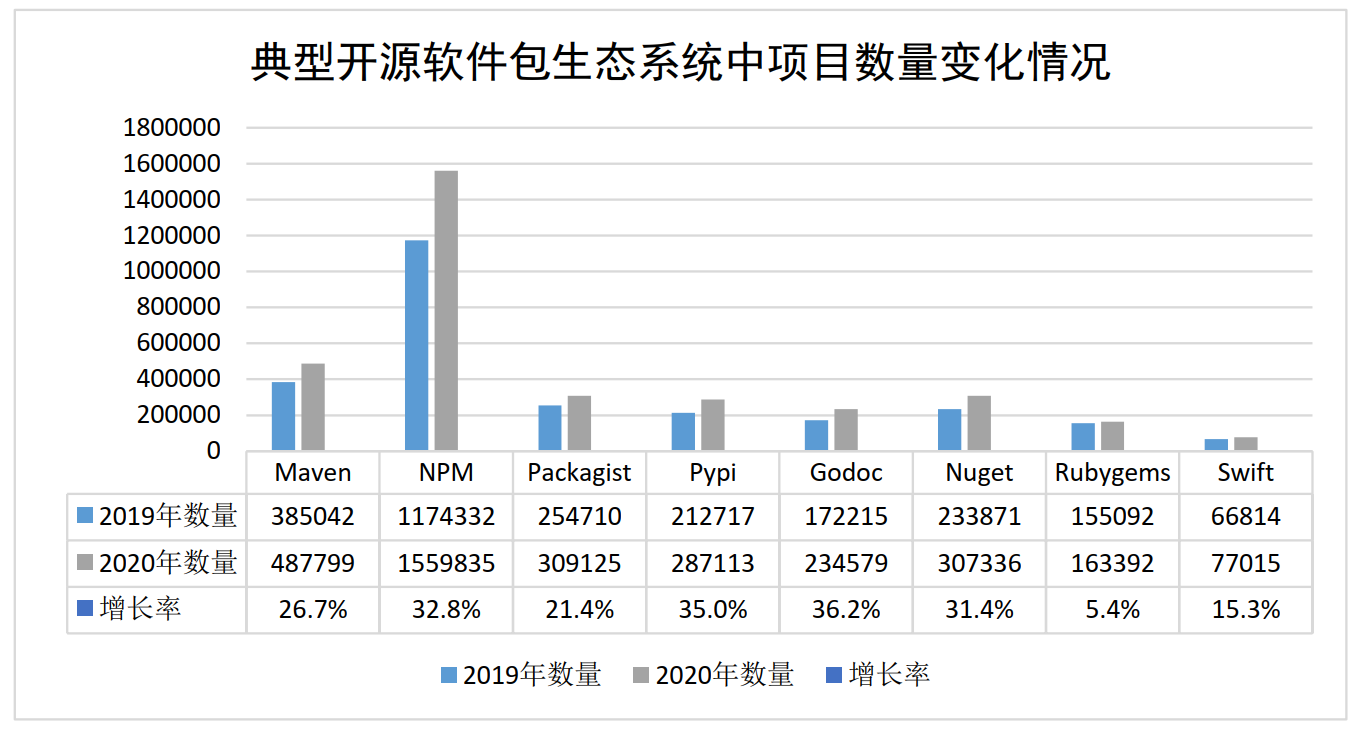
\includegraphics[height=3cm]{qianxin.png}
    \caption{2019和2020年八个典型开源软件包生态系统的增长情况}
	\label{fig:qianxin}
  \end{subfigure}
  \hspace{1cm}
  \begin{subfigure}{0.3\textwidth}
    \centering
    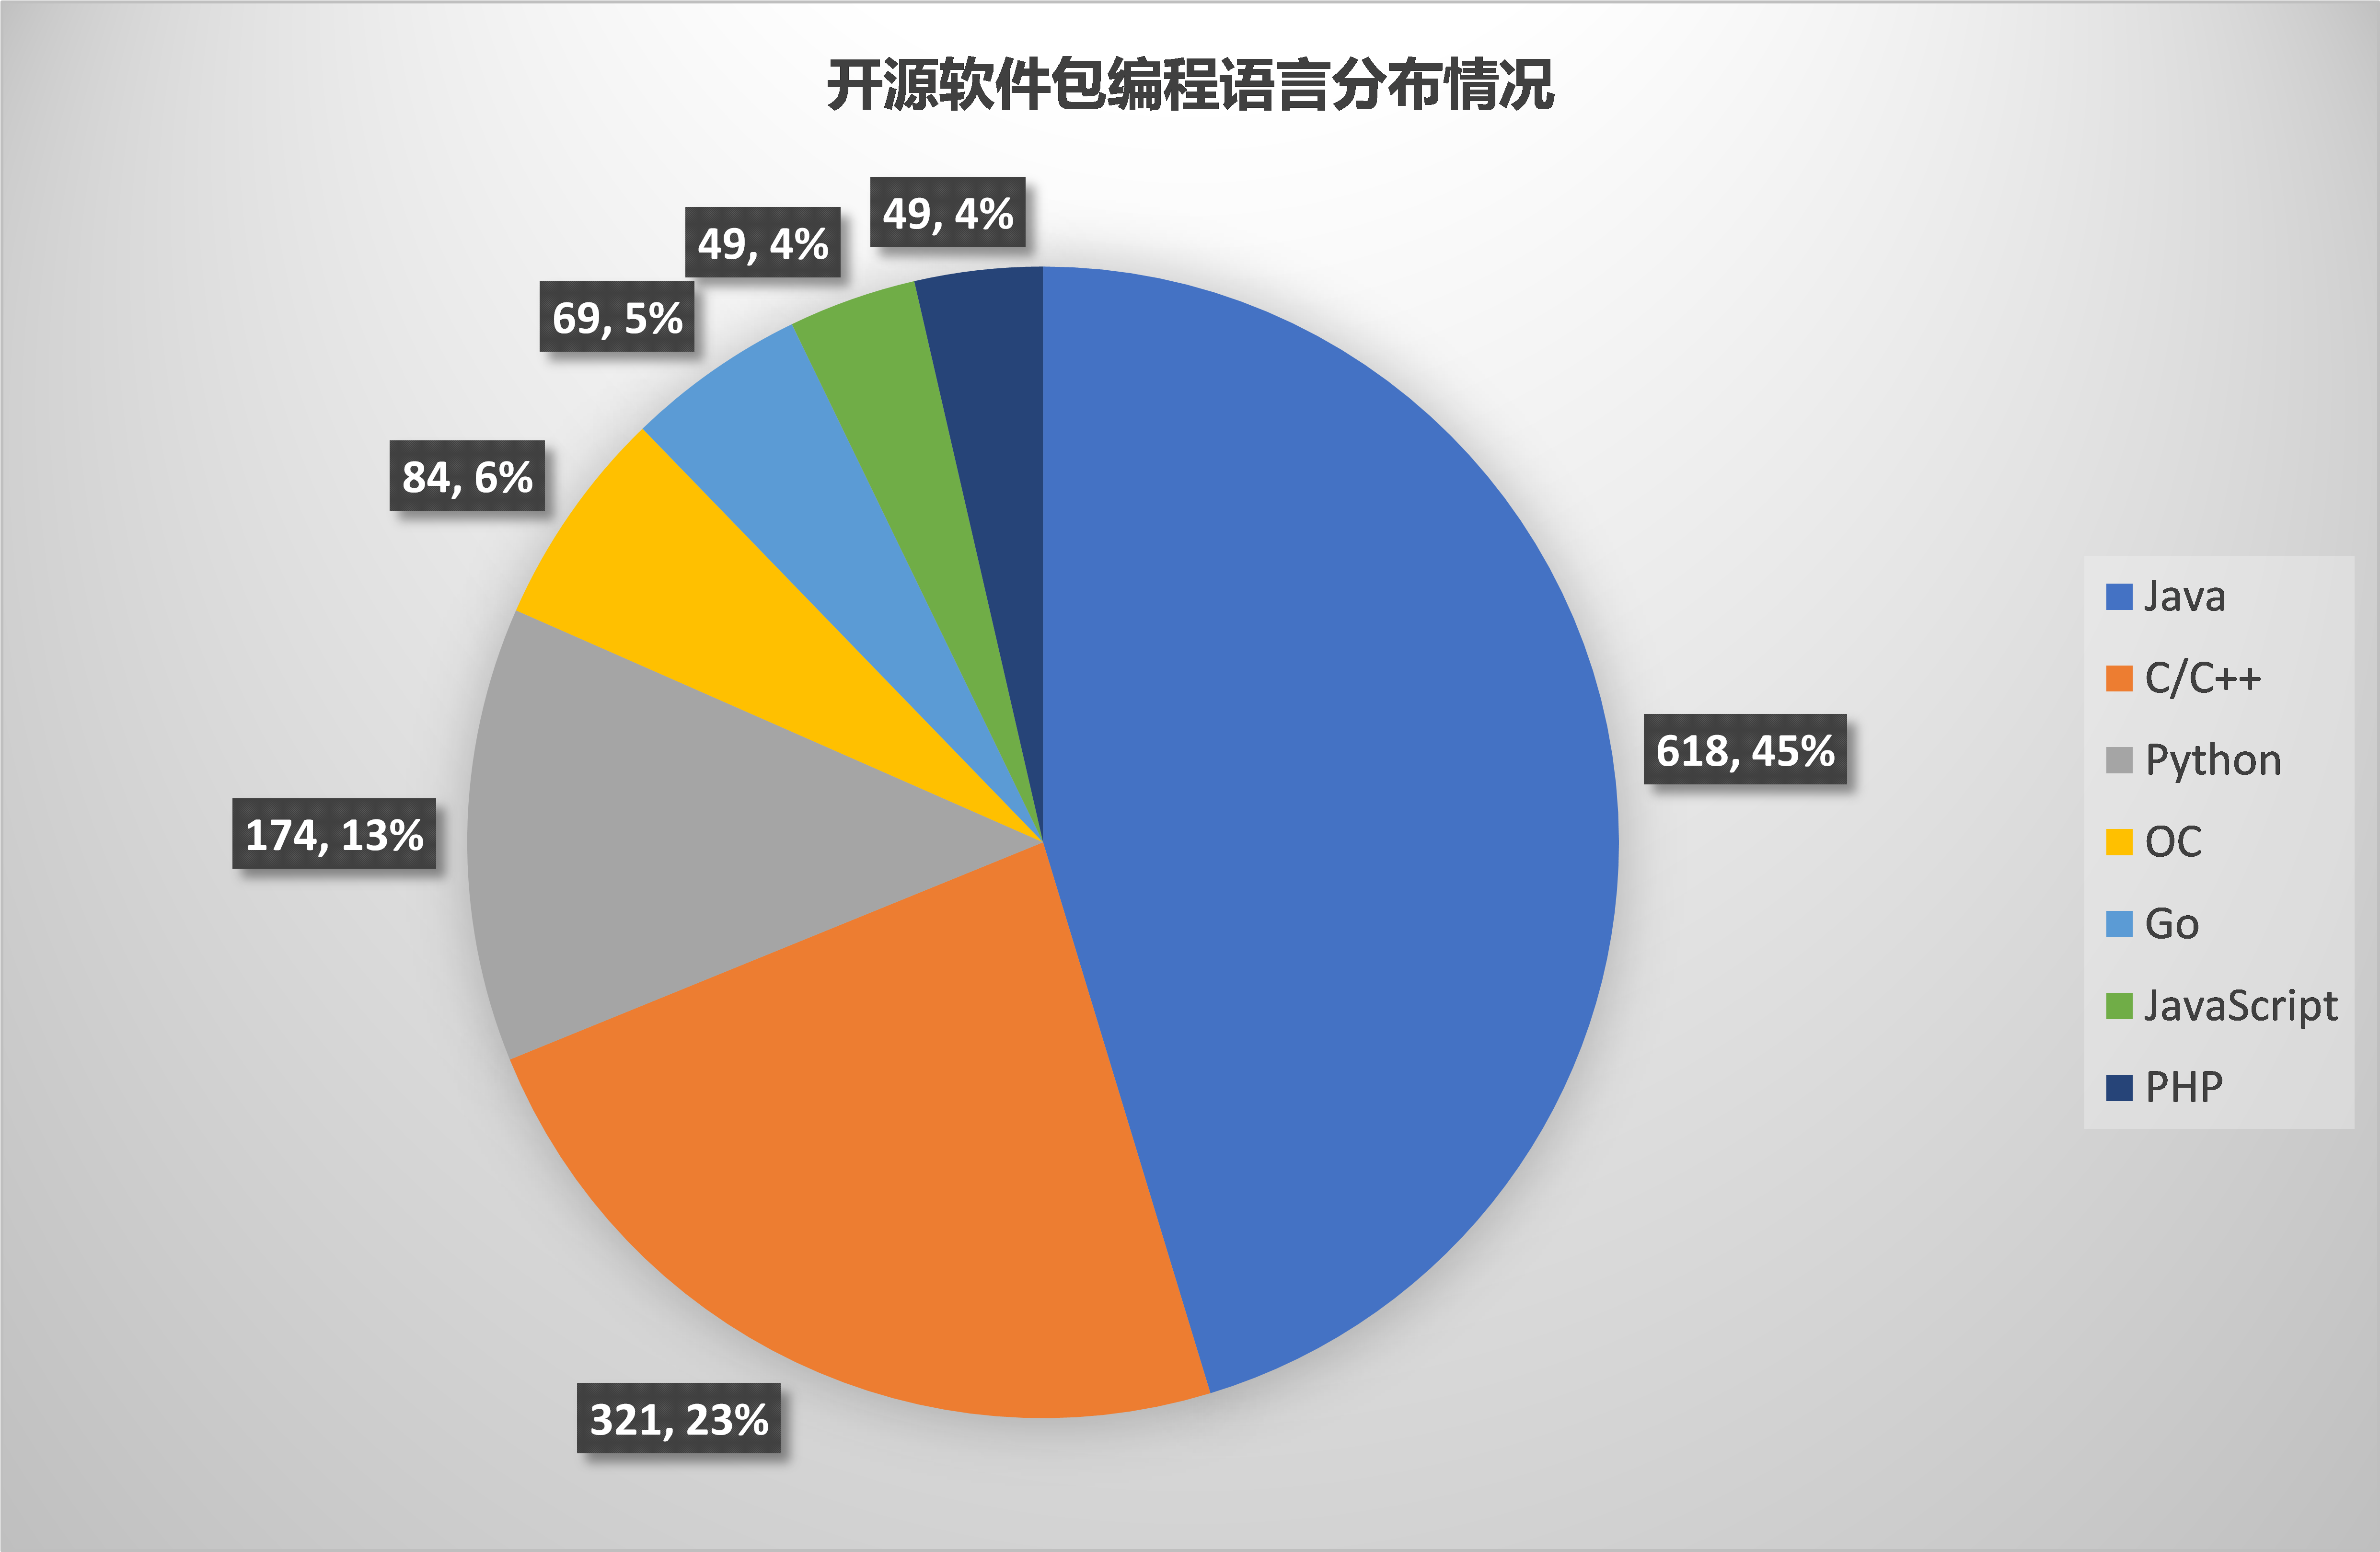
\includegraphics[height=3cm]{language.png}
    \caption{八个典型开源软件包生态系统的1364个项目的编程语言分布情况}
	\label{fig:language}
  \end{subfigure}
  \caption{奇安信对八个典型开源软件包生态系统的增长情况与编程语言分布的统计结果}
  \label{fig:subfigure}
\end{figure}

Maven、Nuget、NPM包生态系统的开源项目进展速度尤为突出,开源项目的平均版本数超过了11个。如表所示\ref{tab:version},八个典型的开源软件包生态系统的开源项目数量和版本数量如表所示。其中Maven包生态系统高居榜首,每个项目的版本数平均值为18.0,Nuget包生态系统和NPM包生态系统分别位于第二和第三,平均值分别为11.0和9.8\cite{qianxin.com}。

\begin{table}[!hpt]
  \caption{奇安信实验室统计的八个典型的开源软件包生态系统的项目数量和版本数量}
  \label{tab:version}
  \centering
  \begin{tabular}{cccc} \toprule
%    \multicolumn{2}{c}{Item} \\ \cmidrule(r){1-2}
    包生态系统 & 项目数 & 版本数 & 平均版本数 \\ \midrule
	Maven & 487799 & 8785416 & 18.0 \\
	NPM & 1559835 & 17148119 & 11.0 \\
	Packagist & 309125 & 3035815 & 9.8 \\
	Pypi & 287113 & 2419533 & 8.4 \\
	Godoc & 234579 & 1109833 & 4.7 \\
	Nuget & 307336 & 3588880 & 11.7 \\
	Rubygems & 163392 & 1094135 & 6.7 \\
	Swift & 77015 & 474314 & 6.2 \\ \bottomrule
  \end{tabular}
\end{table}

如图\ref{fig:language}所示,在检测的1364个开源项目中,所涉及的7个编程语言Java、C/C++、Python、OC、Go、JavaScript、PHP里Java项目数为618,占据了45\%的最高比例。




\section{软件供应链安全现状及研究意义}
软件供应链的上游软件可能悄无声息地影响着下游产品。开源软件之间的依赖关系错综复杂,因此在开发过程中,大多数开发者会选择使用包管理程序来实现自动管理,这可能导致在开发人员未意识到的情况下大量的开源软件被引入产品。一旦某个上游的开源软件被发现安全漏洞,而软件开发者又无法即时发觉产品受到影响,就会隐含巨大的软件供应链安全风险。

2020年5月,GitHub披露了Octopus Scanner漏洞\cite{octopus},该漏洞是针对Apache NetBeans IDE项目的开源软件供应链攻击,影响到了26个开源项目。

2020 年 12 月,安全公司FireEye发现全球著名的网络安全管理软件供应商 SolarWinds遭遇国家级 APT 团伙高度复杂的供应链攻击。该攻击在SolarWinds的一个数字签名组件DLL中插入后门,该后门通过HTTP协议与第三方服务器通信。

\paragraph{安卓软件的供应链安全} Appbrain\cite{appbrain}追踪了450个流行的库,统计结果显示它们在安卓生态系统中有着广泛的使用,广告库、社交网络库、以及手机设备分析库尤为受欢迎。如此广泛的第三方库使用在加速开发过程、避免重复造轮子的同时,也吸引着攻击者将目标向软件供应链上游移动,通过利用受欢迎的库的漏洞来达到攻击应用的目的。来自Trend Micro的安全研究团队披露百度提供的SDK中的Moplus包含的功能可能被恶意使用,以向用户设备植入后门\cite{baidu}。这一处于软件供应链上游的漏洞已经流入超过14000款安卓APP,可能使得约1亿用户处于黑客的攻击风险中。

2022年4月Google Play商店内的安卓应用超过260万,3月与4月新增应用数量均在2万左右,来自其他市场的应用更是不计其数。

如此数量的APP包含着不可忽视的供应链风险,但是由于APP包含着敏感信息或者具有商业价值的运行逻辑,大部分开发者基于安全和产权的考虑都会将产品进行混淆后再发布。这导致在对APP进行安全性检查时更加困难,识别混淆APP中引入的上游软件成为了亟待解决的问题。事实上,约78\%的漏洞都是在间接的依赖中找到,可能带来的安全风险则更加难以发现\cite{qianxin.com}。


\section{研究内容和主要贡献}
在软件供应链的范畴内,本课题选择安卓软件供应链中Java语言的开源仓库组件的识别与分析作为主要目标,设计了应用市场App与标准库数据库的特征提取及匹配方法。对来自App/标准库的包,根据目录信息构建树型结构,根包作为树的根节点,类作为中层节点,方法设置为叶子节点。以树为基础,自下而上提取特征信息,精确度达到方法级别。充分考虑到当前App混淆技术的成熟,在特征的提取过程所有的名称常量都被过滤掉,同时目录的结构也被最大程度简化。为了在高层特征中体现出低层特征,本文引入了模糊哈希算法;同时为了加快特征信息的匹配速度,还采用了分级特征匹配的策略以及用于优先匹配的优先级队列。

本文的主要贡献如下:

\begin{enumerate}
\item{本文提出识别能力精确到具体版本的第三方库检测系统TPL-V Detector,实现了高准确率、高召回率、低误报率的检测方法。}
\item{本文提出基于描述符类型以及字节码指令序列的特征生成方法,使得TPL-V Detector在检测混淆App方面仍有较好的表现。}
\item{本文引入了粗/细粒度两级特征,并在数据库匹配过程中加入优先级队列策略,有效优化了朴素的匹配方法,节省了时间开销。}
\item{本文在Maven数据集上进行了评估,能够准确将混淆前后的SDK一一匹配,在6个库超过200个版本的情况下实现了100\%的准确率。}
\item{本文在App数据集上进行了实验测试,详细分析了不同阶段的时间开销,在综合版本识别与准确率等多个因素考虑下具有较好的性能,准确率高达98.9\%。}
\end{enumerate}


\section{论文内容安排}
本文介绍了TPL-V Detector——上游Java开源仓库的标准组件及其版本在下游混淆App产品中的检测工具的设计、实现以及性能评估。

\paragraph{第一章}简要介绍了软件供应链的蓬勃发展现状,以及当前产品开发流程中对标准组件的高重用;接着以近年来所发生的针对软件供应链的较为严重的攻击事件,阐述了其安全风险的影响范围之广,影响程度之深,表明了该问题的紧迫性和严重性。最后,提出了本课题基于这一背景的研究内容和主要贡献。
\paragraph{第二章}介绍了常用的App混淆技术及其对App中第三方库识别带来的困难;继续分为混淆库检测、无先验知识检测和有先验知识检测三个类别简述了研究现状,讨论不同类别检测方法的基本特征;最后针对版本检测问题,论述了目前方法的匮乏以及面临的主要问题。
\paragraph{第三章}详细叙述了TPL-V Detector的系统设计和实现流程。首先提出了研究方法的总体架构,然后从App的预处理、特征树构建、特征存储与特征匹配几个步骤作了详细介绍。其中还补充了安卓应用各类文件的技术背景,并对特征树的结构、匹配流程与匹配策略等关键技术点增加了流程图与伪代码算法来辅助说明。
\paragraph{第四章}针对准确率、召回率、FPR等指标,对TPL-V Detector的表现进行了评估,此外还深入分析了其各个阶段的时间开销,以及导致各种数据结果的可能原因。最后与现有工具进行了准确率和时间开销的比较。
\paragraph{第五章}总结本课题的主要贡献,分析TPL-V Detector的优越性与不足之处,提出可能的原因以及现存的改进点,探讨值得后续深入研究的问题,提出展望。


\chapter{技术背景}

\section{App混淆技术}
App的混淆技术通常指代码混淆(Code Obfuscation),是将程序中的代码以某种规则转换为难以阅读和理解的代码的一种行为。为了有效保护开发人员的知识产权,代码混淆技术被广泛地应用于各类App产品中。混淆的好处在于:它令Apk的逆向难度变大,提高了了反编译的成本。此外Android当中的混淆还可以移除未使用到的资源,例如第三方库中未使用到的部分或者逻辑上存在的永远不会执行到的死代码,能够显著减小Apk体积\cite{dong2018understanding}。

\subsection{混淆工具Proguard}
Java平台提供了混淆工具Proguard\cite{proguard}来帮助开发者快速对代码进行混淆,对Proguard的描述如下:
\begin{enumerate}
\item{它是一个包含代码文件压缩、优化、混淆和校验等功能的工具。}
\item{它能够检测并删除无用的类、变量、方法和属性。}
\item{它能够优化字节码并删除未使用的指令。}
\item{它能够将类、变量和方法的名字重命名为无意义的名称从而达到混淆效果。}
\item{它会校验处理后的代码,主要针对Java\ 6以上的版本和Java\ ME。}
\end{enumerate}

Proguard的工作流程由压缩(shrink)、优化(optimize)、混淆(obfuscate)和预验证(preverify)四个步骤组成,如图\ref{fig:proguard}所示,每个步骤都是可选的,用户可以通过配置脚本来决定执行其中的哪几个步骤\cite{csdn}。

\begin{figure}[!htp]
  \centering
  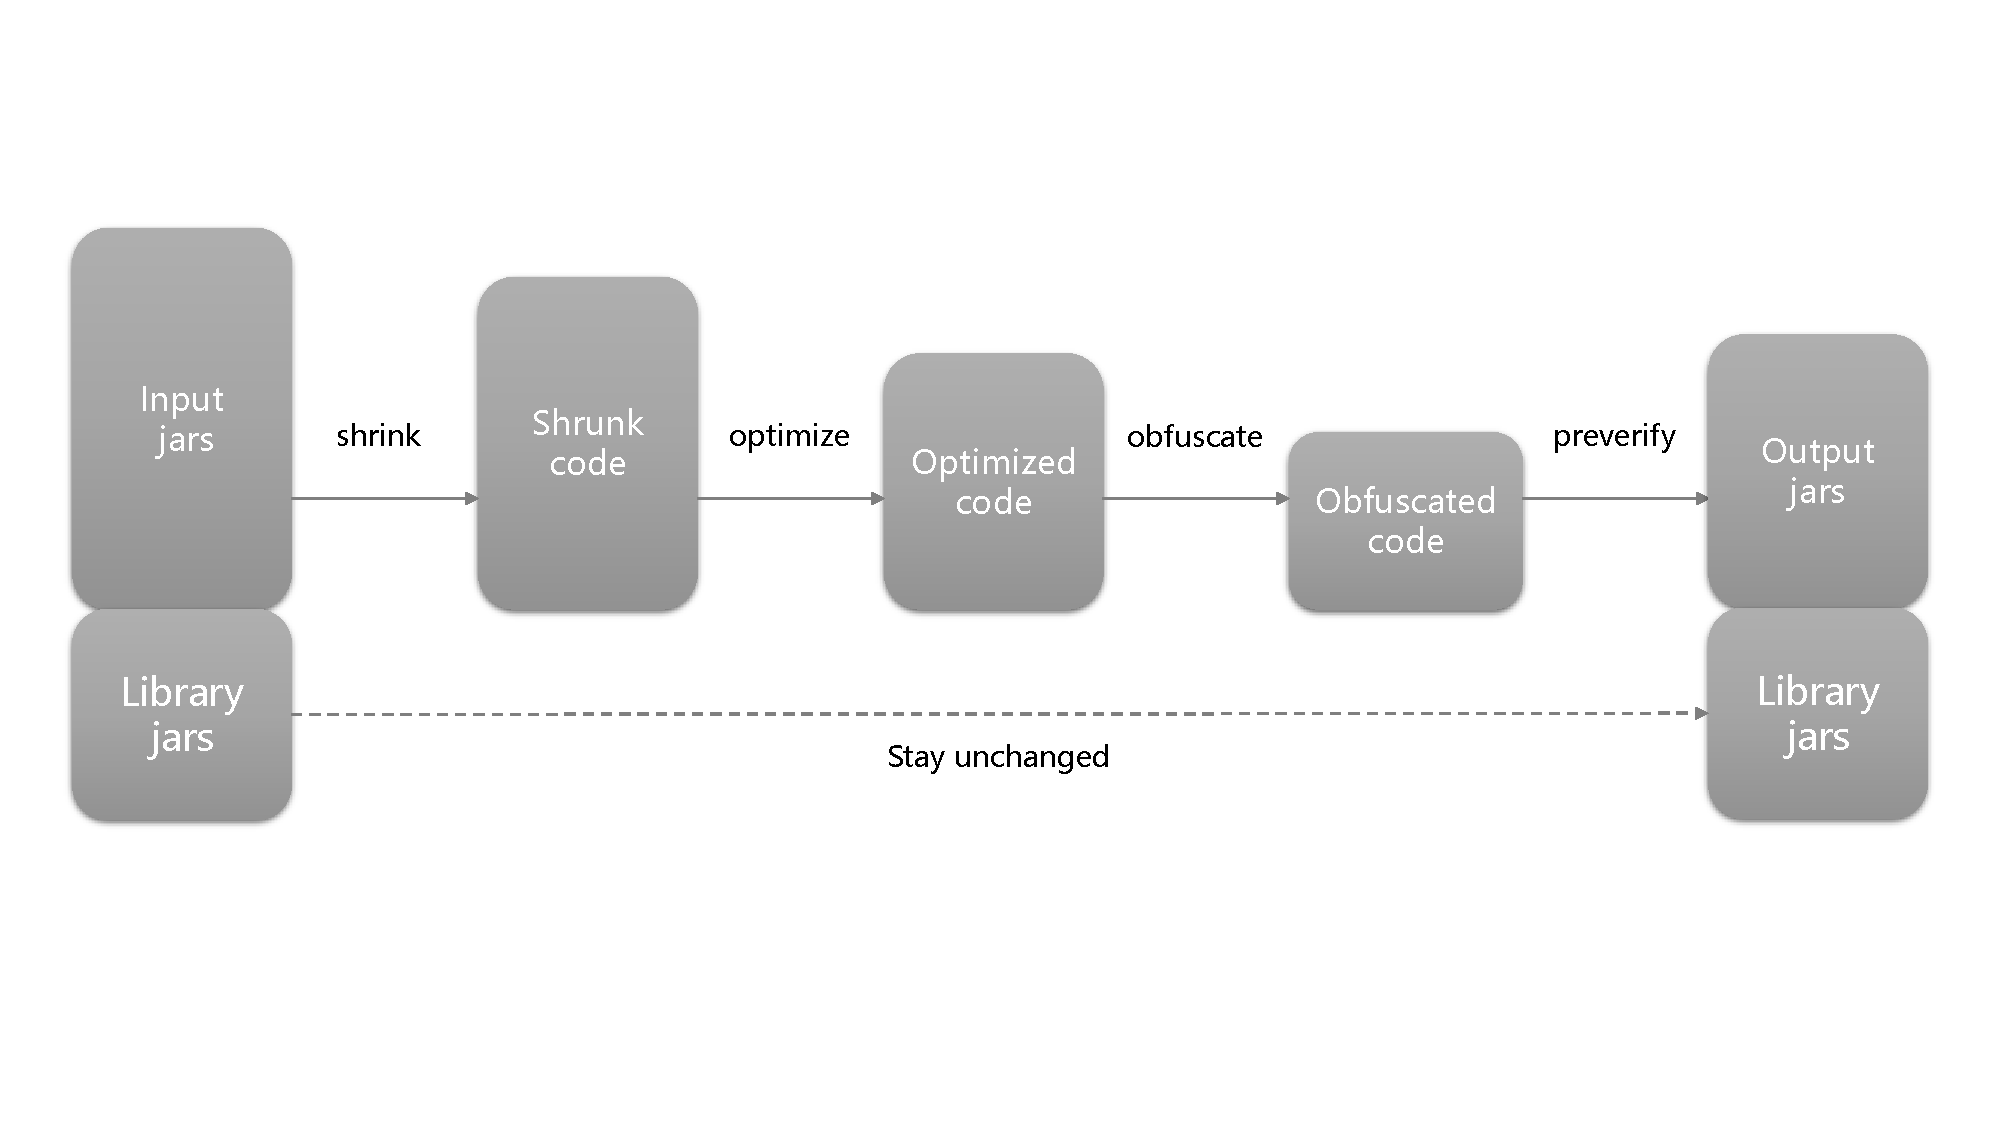
\includegraphics[width=14cm]{proguard.pdf} \\
  \caption{流行混淆工具Proguard的工作流程}
 \label{fig:proguard}
\end{figure}


\subsection{标识符混淆}
标识符混淆通常指将类、变量和方法的名字重命名为无意义的名称。从一款来自360的经过混淆处理的Apk得到的class文件如图\ref{fig:hunxiao}所示,文件名被重命名为简短、无意义的字母组合,相应的源代码中引入这些类的\textit{import}语句也被混淆处理。从名称中无法获取任何信息。在静态链接方法下,开发人员将第三方标准库代码下载到本地,统一打包为Jar文件,代码混淆不仅可以应用于开发者代码,也可以应用于第三方代码,达到隐藏依赖的目的。对于攻击者而言,可以通过恶意引入被披露包含漏洞的一些标准库的旧版本,来达到向App中秘密植入漏洞的目的\cite{hammad2018large}。

\begin{figure}[!htp]
  \centering
  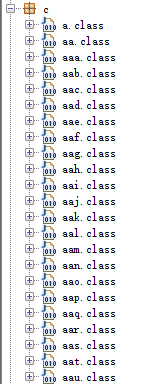
\includegraphics[width=3cm]{hunxiao.png} \\
  \caption{一款360软件的apk解压后得到的经过重命名混淆的class文件}
 \label{fig:hunxiao}
\end{figure}

\subsection{花指令}
花指令也叫垃圾指令,是指在原始程序中插入一组无用的字节,同时保持程序的原始逻辑不变,程序仍然可以正常运行,然而反汇编工具在反汇编这些字节时会出错,由此造成反汇编工具失效,提高破解难度\cite{and}。

花指令的主要思想是,当花指令连同正常指令的前几个字节被反汇编工具识别为一条指令时,引起反汇编工具报错。因此插入的花指令都是一些随机的但不完整的指令。不论花指令形式如何,其必须满足两个基本条件:
\begin{enumerate}
\item{在程序运行时,花指令位于一个永远不会被执行的路径中。}
\item{花指令也是合法指令的一部分,只不过它们是不完整的指令。}
\end{enumerate}

据此,需要在每个要保护的代码块之前插入无条件分支语句和花指令,无条件分支保证了程序在运行时不会运行到花指令的位置,从而引起反汇编工具在进行反汇编时报错。目前的反汇编工具主要分为两类:线性扫描算法和递归扫描算法。线性扫描算法按顺序逐个将每一条指令反汇编成汇编指令,因此会把花指令错误识别,导致程序出错\cite{huazhiling}。递归扫描逐个反汇编指令,如果某个地方出现了分支,就会把这个分支地址记录下来,然后对反汇编过程中碰到的分支进行反汇编,因此反汇编能力更强。

\subsection{控制流平坦化}
控制流平坦化,就是在不改变源代码的功能前提下,将代码中的if、while、for、do等控制语句转换成switch分支语句。这样做的好处是可以模糊switch中case代码块之间的关系,从而增加分析难度\cite{balachandran2016control}\cite{laszlo2009obfuscating}。

这种技术的思想是,首先将要实现平坦化的方法分成多个基本块——即case代码块,和一个入口块,为每个基本块编号,并让这些基本块都有共同的前驱模块和后继模块。前驱模块主要是进行基本块的分发,分发通过改变switch变量来实现。后继模块也可用于更新switch变量的值,并跳转到switch开始处\cite{王柯林2021基于随机森林的抗混淆}。





\section{第三方库检测研究现状}

\subsection{检测混淆库}
随着APP混淆技术的成熟,以第三方库能够被容易地区分为前提的方法已不适用,标识符被混淆为无意义的简短的字母组合,比如\textit{com.google}可能被混淆为\textit{a.c},无法提供关于库的任何信息。



T. Book等人的工作通过白名单的方法检测APP内的第三方库\cite{book2013longitudinal},但这类方法显然无法解决标识符重命名的问题。PEDAL\cite{liu2015efficient}借助机器学习方法,从SDK和Apk中提取代码特征,训练分类器来识别广告库。PEDAL首先将原始Apk转换为字节码,对每一个包的目录,计算其内字节码文件的特征,包括安卓基本组件、可选安卓权限、用户界面元素、运行时权限检查的API等方面。预训练的模型用基于这些特征生成的特征向量作为输入,为每一个包打上应用(App)或广告(Ad)的标签。最终PEDAL重写权限逻辑,重装Apk,得到无广告的纯净应用。基于字节码的方法使得PEDAL不受到重命名混淆的影响。


\subsection{检测未知第三方库}

一些研究工作提出了在没有已知第三方代码的数据库知识情况下检测APP组成成分的方法。此类方法通常首先把开发者代码与第三方代码进行区分,再将第三方代码聚类成不同的组件,组件即一个可能的库的候选,进一步评估候选之间的相似度,当超过相似度阈值的候选的出现次数足够多时就认为找到了一个库。

如Chen等人\cite{chen2016following}从大量的APP中获取库,进行聚类和检测。这一方法在混淆的情况下表现不佳,因为其假设不同APP中包含的库的相同实例拥有相同的包名,而混淆打破了这一基本的假设。

Li等人\cite{li2018large}提出了在缺少先验知识的情况下从手机App中提取库的方法。首先综合包含关系、继承关系及调用关系三个因素将App切分成多个部分,两个具有包含或者继承关系的包被定义为{\kaishu 同质包}(Homogeny Package)。再根据包内函数对包外函数的调用关系,将不同的包放入一个集合当中,此集合就作为一个第三方库的候选。对每一个方法,按照其控制流图中的基本块的操作码序列的哈希值生成基本块的特征。接着将基本块的特征排序和连接,生成方法的特征,并以此类推直到生成库级别的特征。用特征来计算库之间的相似度,当某个集合内的候选库满足相互之间的相似度超过预定义的阈值,且集合的规模的足够大时,就认为找到了一个真正的第三方库。这一方法不要求先验知识,能够有效发现新的第三方库,但是只有当数据集中包含足够多的App时才能够使得相似候选库高频率出现。一些不流行的库,即便是来自开源仓库的标准库,也难以检测出来。



为解决包名混淆问题,LibRadar\cite{ma2016libradar}使用特征哈希的方法,不需要基于包名的聚类,而是借助包中的目录结构来识别库的候选,具体来说是将一个候选表示为一个目录树的结构。这引入一个新的假设,即包的结构在混淆过程中不改变。但混淆工具可以将不同的包合并为一个包,很容易打破这一假设。WuKong\cite{wang2015wukong}和AnDarwin\cite{crussell2014andarwin}用控制流图和API数量来定义哈希特征,用来计算各候选库的相似度。考虑到混淆工具可能修改一个方法的控制流图,或者移除在APP运行中未真正使用的方法,哈希的质量影响着这两类方法的表现性能。


\subsection{检测已知第三方库}

基于已知库的检测要求关于现存库的知识,如库的基本信息、哈希特征等,在混淆APP第三方库识别的场景下,用构建知识数据库的代价换取了更好的表现。

LibRoad\cite{xu2020libroad}使用了典型的基于先验知识数据库的检测混淆App第三方库的模型。如图\ref{fig:libroad}所示,LibRoad首先对App目录进行解析,分出经过混淆处理的部分以及未经过混淆处理的部分。对于未经混淆的包,通过包名匹配策略可以轻松从数据库中找到对应的标准库。对于混淆处理的包,LibRoad在类粒度上生成了类签名,同样数据库中的各类也预先生成和存储好了签名。首先进行本地数据库匹配,如果匹配失败则进行在线匹配,若再次失败则暂定为找到了新的三方库,输出到TPL(Third-Party Library) list中。

\begin{figure}[!htp]
  \centering
  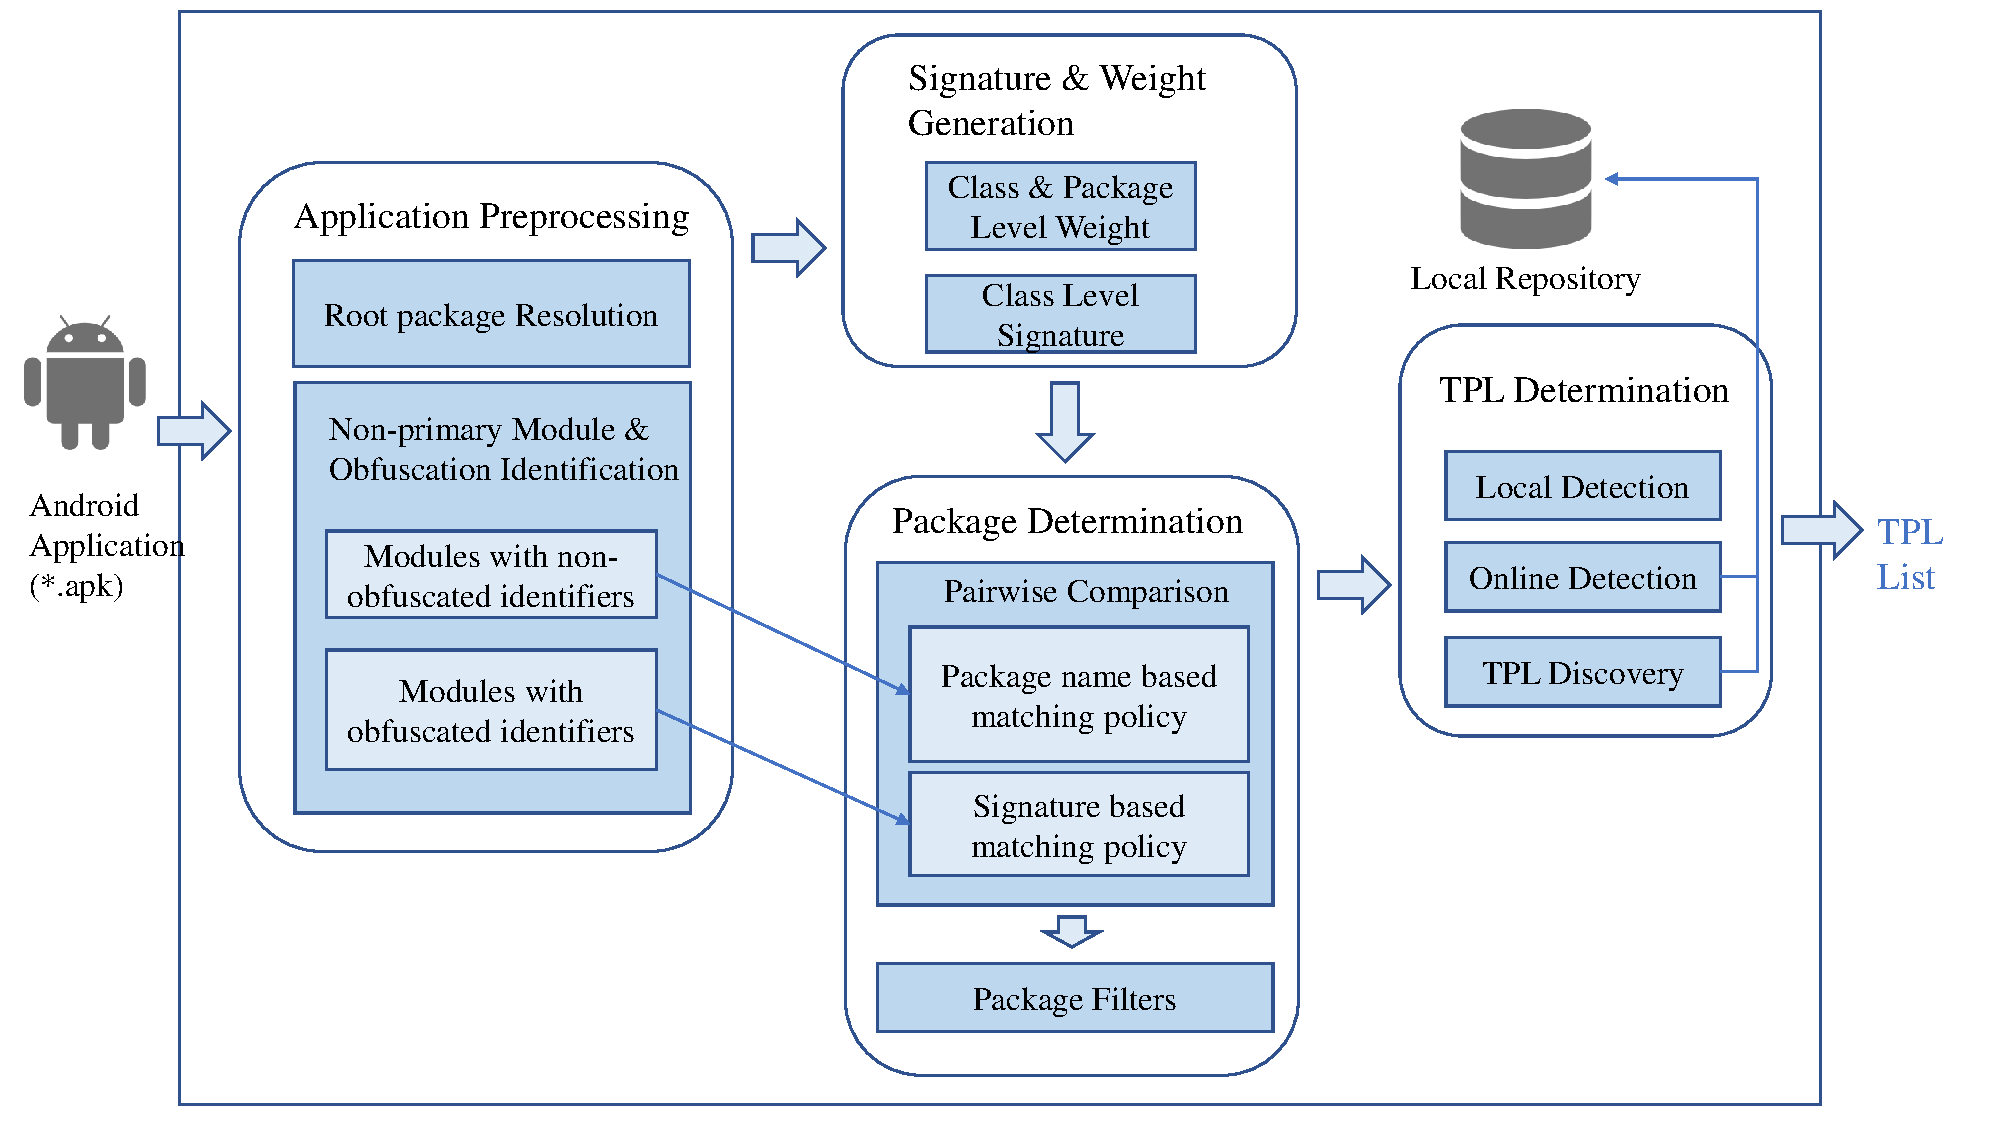
\includegraphics[width=15cm]{libroad.pdf} \\
  \caption{LibRoad的设计框架和工作流程}
 \label{fig:libroad}
\end{figure}

另外一个具有代表性的工具是LibScout\cite{backes2016reliable},将一个包构建为一个Merkel树,根包作为树的根节点,依次往下,方法作为叶子节点。使用Java字节码来计算方法的哈希值作为特征,进一步生成类的哈希作为特征,进行APP与数据库中第三方库的匹配。定义来自标准库的包$lp$与来自App的包$ap$的匹配的得分为
\begin{equation}
score_c(lp,ap)=\frac{\#\ classes\ in\ lp\ that\ match\ in\ ap}{\#\ classes\ in\ lp} \in [0,1]
\end{equation}
超过得分阈值的App的包作为标准库的包的一个匹配候选。为了加速匹配过程,对一个标准库的包$lp$与它的一个匹配候选$ap$,二者拥有相同的根目录结构,因此对于根目录结构不相同的其它候选可以直接剔除。标准库中包与子包的关系也被用来剔除不可能的匹配,以降低计算代价,用$a\ candidateOf\ b$表示$a$是$b$的一个匹配候选,$relationship(a,b)$表示$a$是$b$的父/兄弟/子节点,则剔除不满足以下关系的候选:
\begin{equation}
\begin{aligned}
&\forall \ ap_i,ap_j,lp_x,lp_y,\\
& ap_i\ candidateOf lp_x,ap_j\ candidateOf lp_y,\\
& relationship(ap_i,ap_j)=relationship(lp_x,lp_y)
\end{aligned}
\end{equation}
以上表达式说明,若$ap_i$、$ap_j$分别是$lp_x$、$lp_y$的匹配候选,而对于来自标准库的$lp_x$和$lp_y$所拥有的已知的关系,$ap_i$和$ap_j$之间并不满足同样的关系,则此匹配候选是无效的,不需进一步计算。
最终每个标准库的包在经过筛选后的全局范围内计算得分$simScore$
\begin{equation}
simScore_c=\frac{sum\ of \ matched\ classes}{\#\ of\ classes\ in\ library}
\end{equation}
最大者作为最终匹配结果,即认为该包所属的App中使用了此标准库的包。LibScout生成树形结构,充分利用各个方法特征的特性能够抵抗控制流篡改,同时以字节码和返回值、参数类型为特征,在包/类/描述符重命名情况下依然有效。




\section{第三方库的版本检测}

现有工作中以版本为目标实现精确检测的并不多,AdDetect\cite{narayanan2014addetect}仅能够区分广告和非广告的库,基于聚类的方法如LibRadar\cite{ma2016libradar},LibD\cite{li2017libd}等都没有声明能够检测库的特定版本。

实现版本的检测仍面临着很多问题:
\begin{enumerate}
\item{需要处理庞大的数据集。第三方库本身就纷繁复杂,如果再将各个版本考虑进去,将导致需要处理的数据成倍增长。}
\item{缺乏精确的表示。一个库的不同版本可能差异微小,如何找到合适的特征来区分这一差别非常关键。}
\item{代码混淆的干扰。代码混淆同样会导致库的代码发生改变,这种改变是由不同库引起还是由同一库的不同版本引起,需要被准确的区分。}
\end{enumerate}


\section{本章小节}
本章介绍了本文设计的技术背景,简要叙述了当前安卓第三方库检测的技术分类以及主要特征,提出了版本检测所面临的问题。本章在2.1介绍了App混淆常用的三种技术,从第三方库检测角度说明了混淆技术引入的新的问题。2.2节将现有研究技术分为有先验知识和无先验知识两种类别,对每个类别简述了几种研究方法,归纳不同类别所使用的主要方法,其中无先验知识方法大部分基于聚类算法,通过出现频率确定第三方库;有先验知识方法基于特征提取与匹配,借助标准库确定第三方库。2.3节提出了具体版本识别的困难,以及目前工作需要解决的几个问题。第三章将详细介绍本文提出的TPL-V Detector系统的设计细节。



\chapter{TPL-V Detector系统设计}

在参考了多篇文献后,本文提出了一种适用于包的结构混淆、包/类/标识符重命名场景的,基于已知标准库的数据库,利用两类信息生成粗粒度/细粒度两级哈希特征的安卓应用第三方库及其特定版本的检测系统TPL-V Detector(Third Party Library - Version Detector)。



\section{TPL-V Detector总体架构}

TPL-V Detector不依赖于包中的目录结构以及各级名称,可以抵抗结构混淆和重命名混淆,能够识别第三方库及具体版本。图\ref{fig:arch}展示了系统的四个步骤:
\begin{enumerate}
\item{预处理jar和apk。将来自Maven仓库的jar包以及待检测apk处理成便于构建树结构的形式。}
\item{构建特征树。根据上一阶段输出,将每个包作为根节点构建特征树,该包内的所有类,不论是根包的类还是子包的类,一律作为树的中间层节点,各类的方法作为叶子节点。特征分为粗粒度、细粒度两级特征。粗粒度特征为方法的描述符的返回值以及参数类型,细粒度特征为该方法的字节码,首先生成叶子节点的两级特征,再利用叶子节点生成中间层节点即类节点的特征。}
\item{构建数据库与匹配。根据以上特征生成方法,计算Maven仓库中的标准库的特征,并存储到数据库中。对待检测APP,首先生成粗粒度特征,确定所包含的库,再根据细粒度特征,确定各库的具体版本。}
\end{enumerate}


\begin{figure}[!htp]
  \centering
  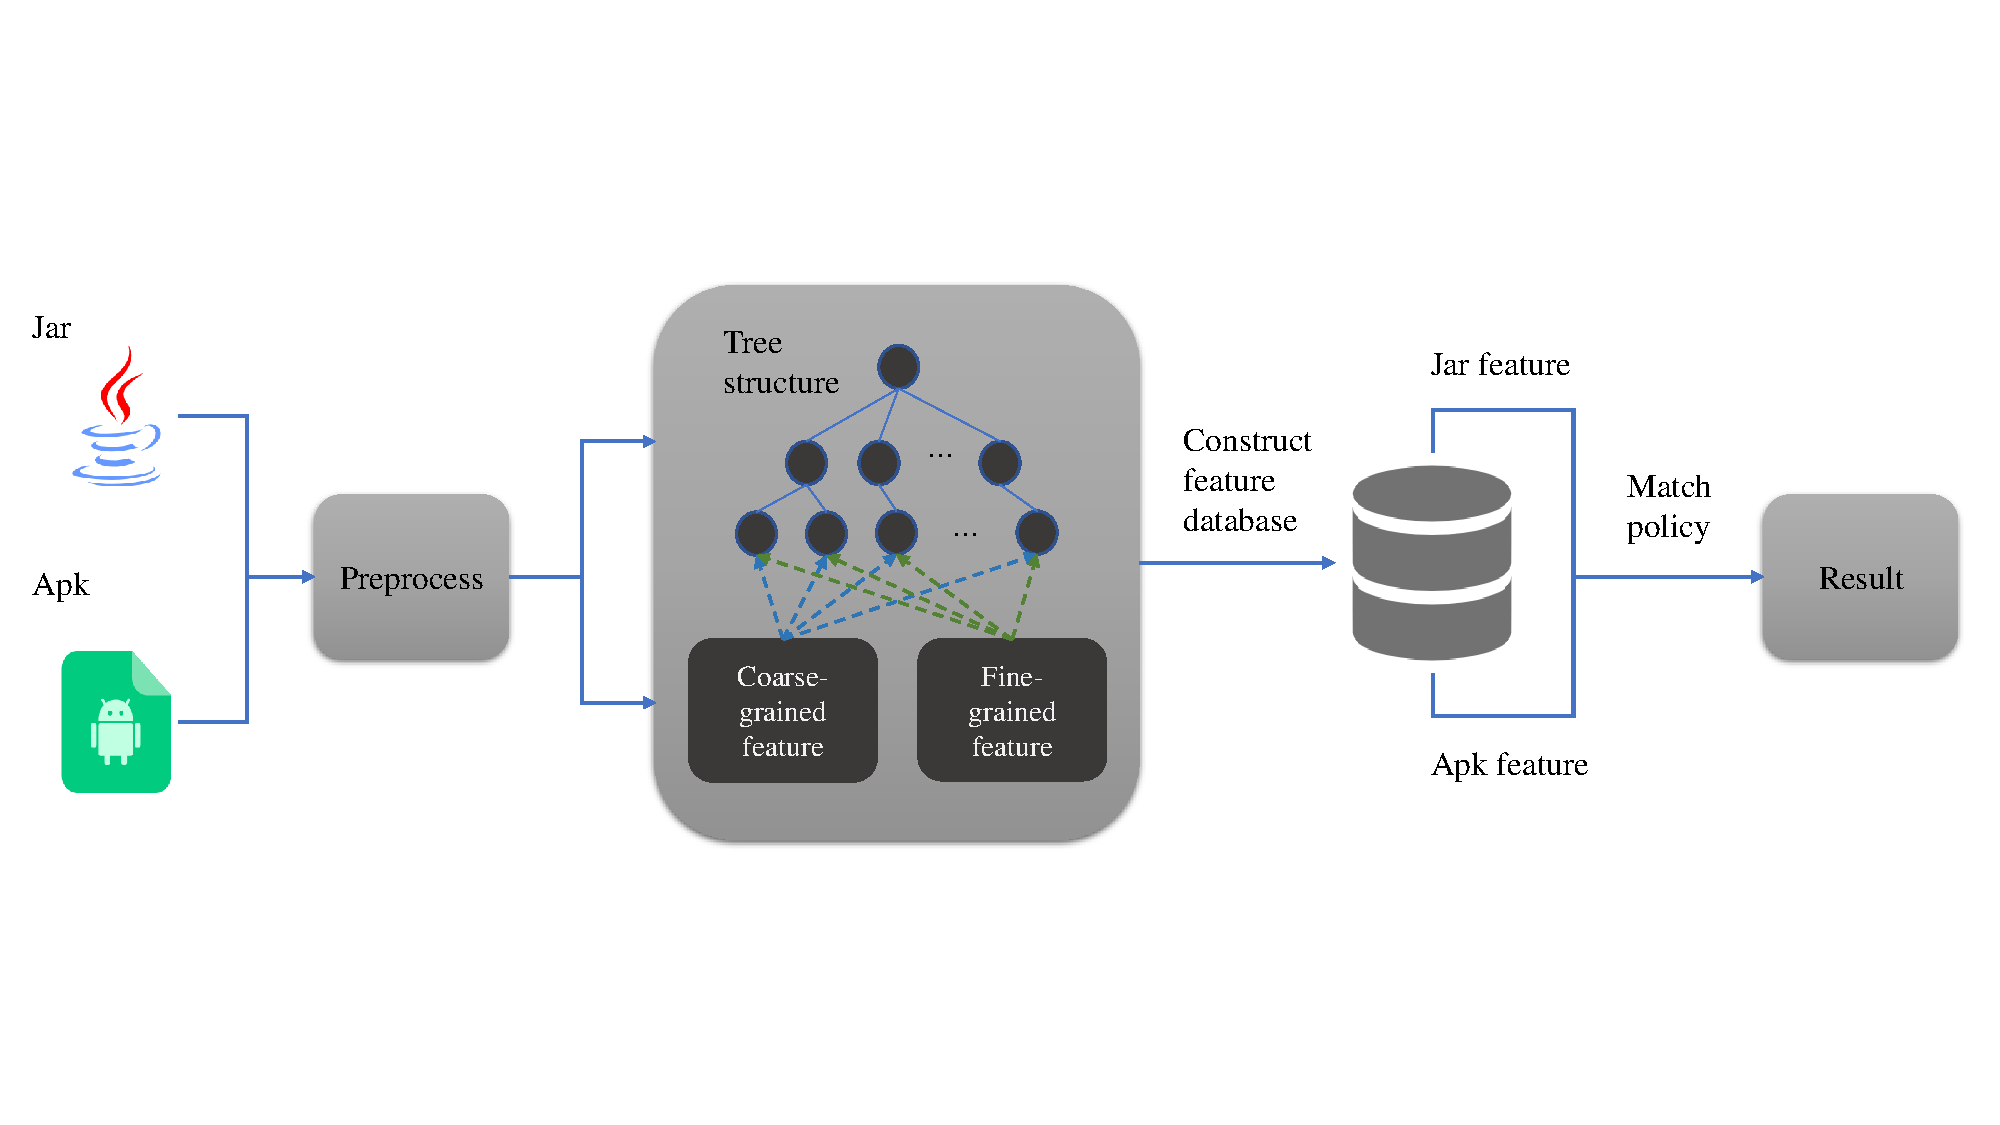
\includegraphics[width=15cm]{arch.pdf} \\
  \caption{TPL-V Detector的总体架构}
 \label{fig:arch}
\end{figure}


\section{包的预处理}


\subsection{Dex与Class简介}

\paragraph{DEX文件}是Android系统中的一种文件,是一种特殊的数据格式,能够被Dalvik虚拟机识别并加载执行,类似于Windows上的EXE可执行文件。将APK安装包解压后得到的文件就包含了DEX文件,它记载了应用程序的全部操作指令以及运行时数据。当java程序编译成class文件后,还需要使用dx工具将所有的class文件整合到一个DEX文件里,目的是其中各个类能够共享数据,在一定程度上降低了冗余,同时也使文件结构更加紧凑。DEX文件大小通常是传统jar包的50\%左右\cite{10min}。


\paragraph{CLASS文件}是能够被java虚拟机识别,加载并执行的文件格式,通过javac程序可以从java源文件生成class文件。class文件记录了一个类文件的所有信息,不仅包含了java源代码中的信息,还包括了this、super等关键字的信息。作为一种8位字节的二进制流文件,class中的数据按顺序紧密排列,没有间隙,从而让JVM加载更加迅速,每一个类、接口或者枚举都单独占据一个class文件\cite{class}。


\subsection{Apk与jar的预处理}

预处理流程如图\ref{fig:preprocess}所示。
\begin{figure}[!htp]
  \centering
  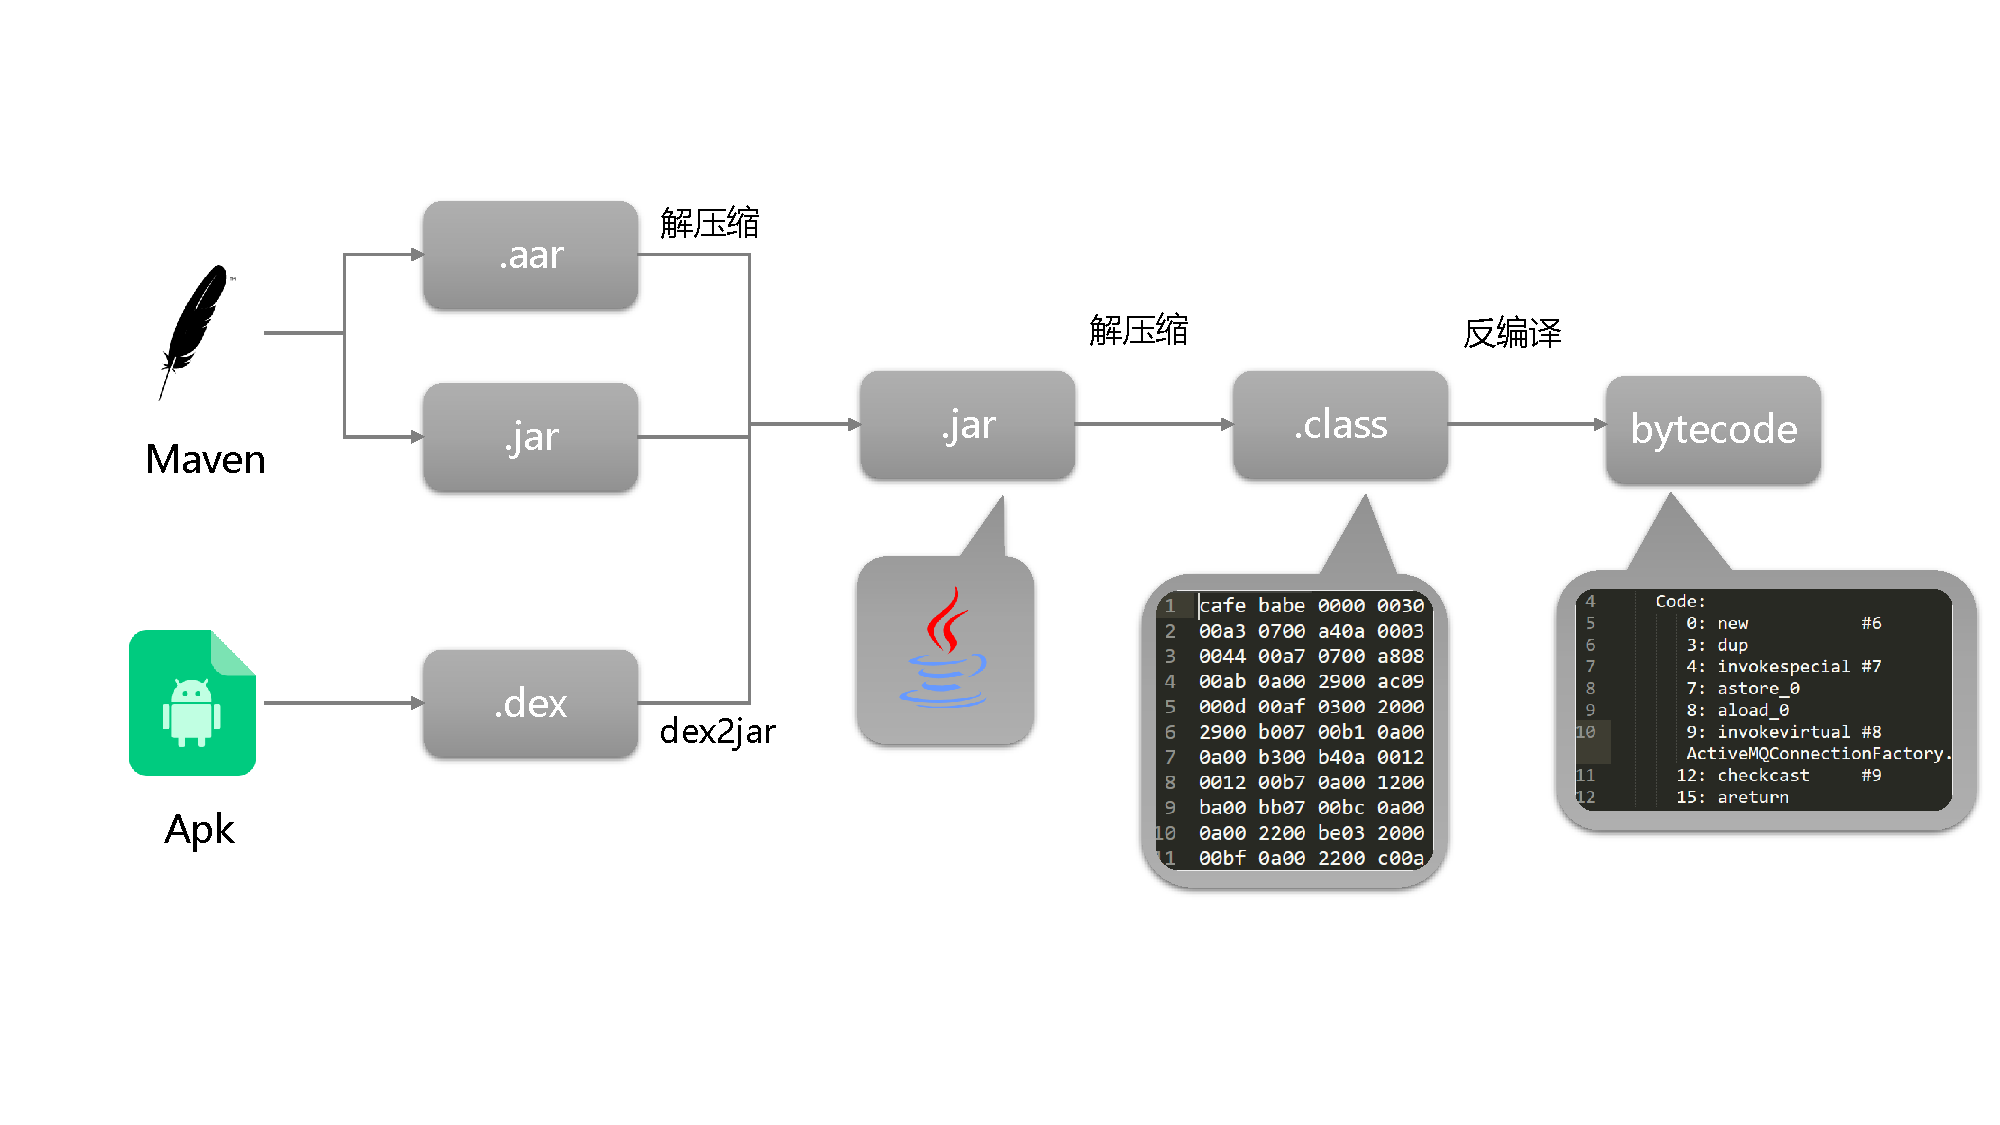
\includegraphics[width=15cm]{preprocess.pdf} \\
  \caption{Apk与标准库转换到java字节码的预处理流程}
 \label{fig:preprocess}
\end{figure}

\paragraph{Apk预处理:}从应用市场获取待检测的应用的安装包,即apk文件。Apk文件本质上为zip格式的压缩文件,解压后可以得到dex文件。借助dex到jar的转换工具dex2jar\cite{d2j}将DEX文件转换为包含多个class文件。此处的class文件通常是经过软件开发者混淆的,大部分类的名称和函数的名称经过了混淆处理,不能提供有效信息,转换得到的包的目录结构也不可靠。


\paragraph{Jar预处理:}Maven社区提供的中央仓库\cite{maven}包含了大量常用的库,包括绝大多数流行的Java开源构件,源码,许可证信息等,一般来说简单的Java项目依赖的构建都可以满足,因此选择Maven仓库中的部分jar包作为构建数据库的基础。我利用爬虫从Maven中央仓库中获取了大量的jar包,将jar包解压就可以获得该标准库的各个class文件。在爬取标准库的过程中,需要跳过一些带有javadoc或者sources字样的链接,这表示该包为一个说明文档包或者源代码包,在此次课题中用不到。


\paragraph{字节码的生成:}Java字节码是一种程序的低级表示,能够直接被java虚拟机所理解和翻译,以实现java跨平台的特性。具有二进制格式的class文件,实质上就是java的字节码,属于独立于平台和操作系统的指令集。为了删除class文件中的常量信息,我使用javap程序将class文件反编译为具有可读性的助记符形式的字节码,可以清楚地区分开描述符,代码,常量池等部分,并存储为文本文件供后续使用。




\section{构建特征树}

\subsection{两级特征}
如果特征的计算方法过于复杂,将会导致在获取apk特征时用时过长,因此本方法中采用了两级特征——粗粒度特征与细粒度特征,来解决这一问题,同时实现第三方库的版本检测。粗粒度特征计算方法简短、生成速度快、相应的精准度有所下降,用于确定待测apk中的包是数据库中的哪一个标准库。细粒度特征计算方法复杂、生成速度慢、但可以精确到单条字节码操作指令的层面。对于细粒度特征而言,即便同一个库的版本不同所导致的细微代码差异也能够体现出来,因此可以在包成功匹配的情况下进一步匹配具体版本。


\subsubsection{粗粒度特征}

粗粒度特征由函数的描述符生成,由于函数描述符包含了函数名、参数名,极易受到重命名混淆影响,因此我将名称部分删去,以\textit{返回值类型 (参数1类型,参数2类型,...,参数n类型)}的字符串作为描述符,计算其md5哈希值,得到该方法的签名,一个例子如表\ref{tab:descriptor}所示。尽管此签名可能在多个包中,乃至一个包中的不同类中出现,但是结合该类下的各个方法的签名,方法的序列,可以减少碰撞的概率,用于初步表示一个类。如表\ref{tab:activemq}所示,标准库\textit{org.codehaus.avtivemq}的两个类\textit{ActiveMQMessageConsumer}和\textit{BrokerClientImpl}在方法“\textit{public java.lang.String toString()}”上发生了碰撞,但是在其他方法上有很大差异,方法的总数也不同,从而类的层面的特征有所区别。


\begin{table}[!hpt]
  \caption{方法描述符的处理}
  \label{tab:descriptor}
  \centering
  \begin{tabular}{cp{8cm}} \toprule
%    \multicolumn{2}{c}{Item} \\ \cmidrule(r){1-2}
    原始描述符 & public static ActiveMQConnection makeConnection(String user, String password, String uri)\\ \midrule
    删除名称后的描述符  & public static org.codehaus.activemq.ActiveMQConnection makeConnection(java.lang.String, java.lang.String, java.lang.String) \\ \midrule
    md5哈希值      & befc542005082b1940176d89035826ab \\ \bottomrule
  \end{tabular}
\end{table}

\begin{table}[!hpt]
  \caption{标准库org.codehaus.activemq中的两个类包含方法(部分)的情况}
  \label{tab:activemq}
  \centering
  \begin{tabular}{ccc} \toprule
%    \multicolumn{2}{c}{Item} \\ \cmidrule(r){1-2}
    描述符 & ActiveMQMessageConsumer & BrokerClientImpl \\ \midrule
     public java.lang.String toString(); & \ding{51}  & \ding{55} \\ 
     protected long getStartTime(); & \ding{51} & \ding{55} \\
      protected void setBrowser(boolean); & \ding{51} & \ding{55} \\
    public void updateBrokerCapacity(int); & \ding{55} & \ding{51}\\ \bottomrule
  \end{tabular}
\end{table}



\subsubsection{细粒度特征}

细粒度特征基于函数的字节码生成。\textit{ActiveMQConnection}类的一个方法\textit{makeConnection}的字节码如下所示:

\begin{codeblock}[language=C]
  public static org.codehaus.activemq.ActiveMQConnection makeConnection(
  java.lang.String) throws javax.jms.JMSException;
    Code:
       0: new           #6                
       3: dup
       4: aload_0
       5: invokespecial #10                
       8: astore_1
       9: aload_1
      10: invokevirtual #8                
      13: checkcast     #9                
      16: areturn
\end{codeblock}


Java字节码是基于堆栈结构的,上面字节码“Code”部分的每一行对应于一条操作指令,仅仅表示对堆栈的操作,而不包含操作数。源代码中所定义的常量、变量名等静态成员存放在常量池中,因而避免了名称混淆的问题。每一条操作指令对应于一个十六进制的操作码,表\ref{tab:bytecode}展示了部分对应关系及其说明。


\begin{table}[!hpt]
  \caption{Java字节码助记符与十六进制操作码对应关系(部分)}
  \label{tab:bytecode}
  \centering
  \begin{tabular}{ccc} \toprule
%    \multicolumn{2}{c}{Item} \\ \cmidrule(r){1-2}
    助记符 & 操作码 & 说明 \\ \midrule
    new  & 0xbb & 创建一个对象,并将其引用值压入栈顶 \\
	dup & 0x59 & 复制栈顶数值,并将复制值压入栈顶 \\
	aload\_0 & 0x2a & 将第一个引用类型本地变量推送至栈顶 \\
	invokespecial & 0xb7 & 调用超类构造方法,实例初始化方法,私有方法 \\
	astore\_1 & 0x4c & 将栈顶引用型数值存入第二个本地变量 \\
	aload\_1 & 0x2b & 将第一个引用类型本地变量推送至栈顶 \\
	invokevirtual & 0xb6 & 调用实例方法 \\
	checkcast & 0xc0 & 检验类型转换,检验未通过将抛出异常 \\
	areturn & 0xb0 & 从当前方法返回对象引用 \\ \bottomrule
  \end{tabular}
\end{table}




\subsection{特征树的实现}

\subsubsection{字节码特征提取}

如图\ref{fig:tree}所示,字节码解析器布置在树的下方,其接收字节码文件,从文件头开始读入,利用正则表达式匹配每一个函数的描述符。当匹配成功时,表明一个函数的读入即将开始,则解析器依次读取函数描述符和操作指令序列,并将原始特征记录为一个特征对。当读至文件尾时,该class文件代表的类的所有成员函数全部读取完毕,将各特征对传递给上方的树。


\subsubsection{方法层}

方法实现为\textit{mNode}(Method Node)类。根据提取出来的字节码的原始特征,对于每一对粗/细粒度原始特征,生成一个方法节点,对原始特征进行处理。方法节点记录了原始的函数描述符,文件路径等基本信息,同时生成了处理后的特征的MD5哈希值,作为此方法的两级特征。表为\textit{ActiveMQConnection}类中方法\textit{createSession}的各个属性值。

\begin{figure}[!htp]
  \centering
  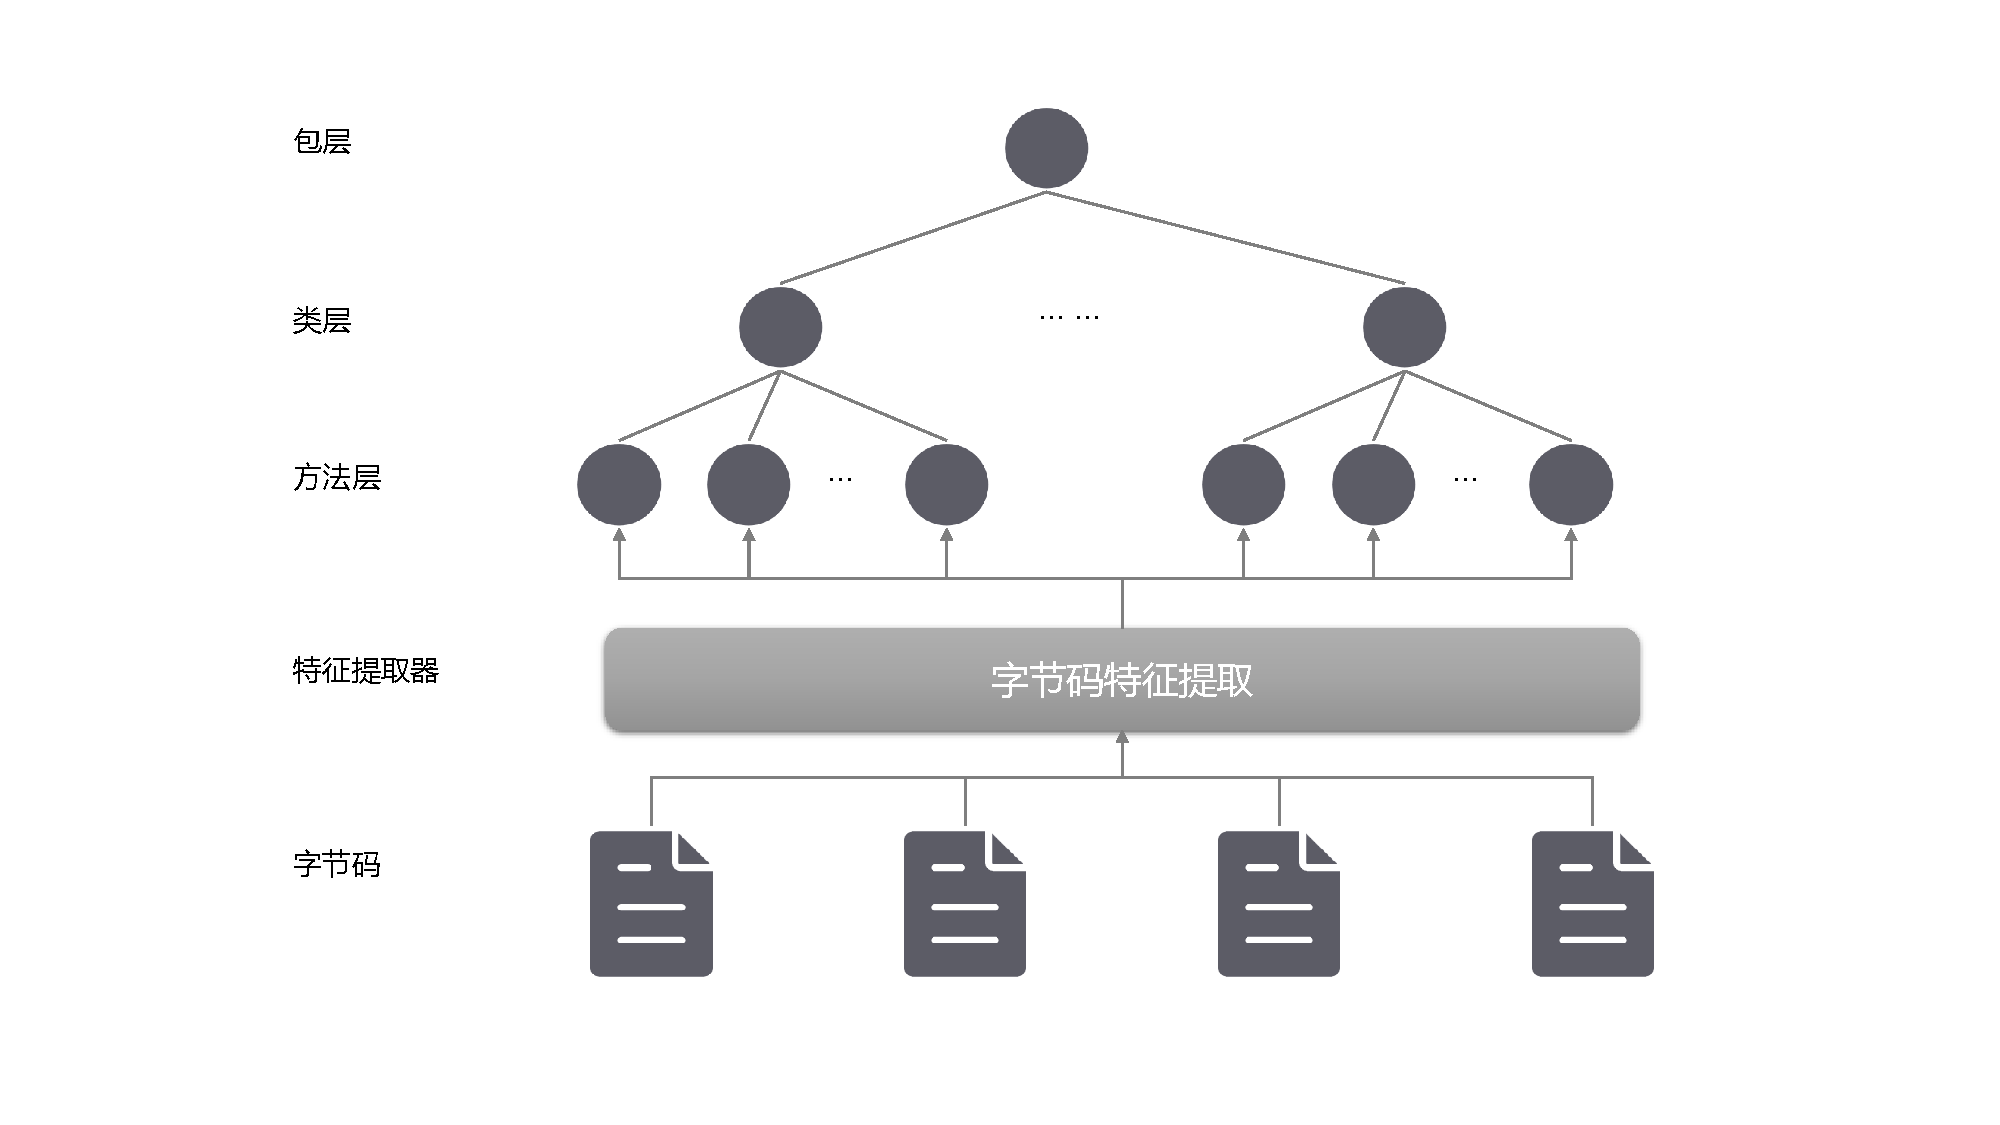
\includegraphics[width=15cm]{tree.pdf} \\
  \caption{使用特征提取器从字节码文件中获取特征并存储为树型数据结构}
 \label{fig:tree}
\end{figure}

\subsubsection{类层}

类实现为\textit{cNode}(Class Node)类,类层根据该class文件中包含的方法,将各个方法对应的\textit{mNode}节点作为自己的子节点。不同类的方法数大相径庭,有的类没有方法,只有数据成员,有的类则包含几十甚至上百个函数成员。再考虑到类的不同版本之间可能差异很小,仅仅体现在个别方法的几个函数上,类的特征必须能体现函数成员的特征。因此我采用了模糊哈希的方法,算法如\ref{algo:fuzzyhash}所示,将类下各方法的特征进行排序、连接,计算模糊哈希值作为类的粗/细粒度特征。

此处模糊哈希的用法与ATVHunter\cite{zhan2021atvhunter}有相似之处,都是为了降低代码混淆对最后特征带来的影响,但是ATVHunter的目标是减少部分指令改变对函数签名的影响,而此处是减少部分函数改变对类的特征的影响。如图\ref{fig:fuzzy}所示,模糊哈希的应用步骤为:
\begin{enumerate}
\item{将类下各方法的特征连接成一个序列。}
\item{使用滑动窗口(滚动哈希)将序列分割成不同的切片。}
\item{对每个切片,计算其MD5哈希值,取最后6位作为压缩映射值。}
\item{最后将所有映射值连接起来作为最终值。}
\end{enumerate}

\begin{figure}[!htp]
  \centering
  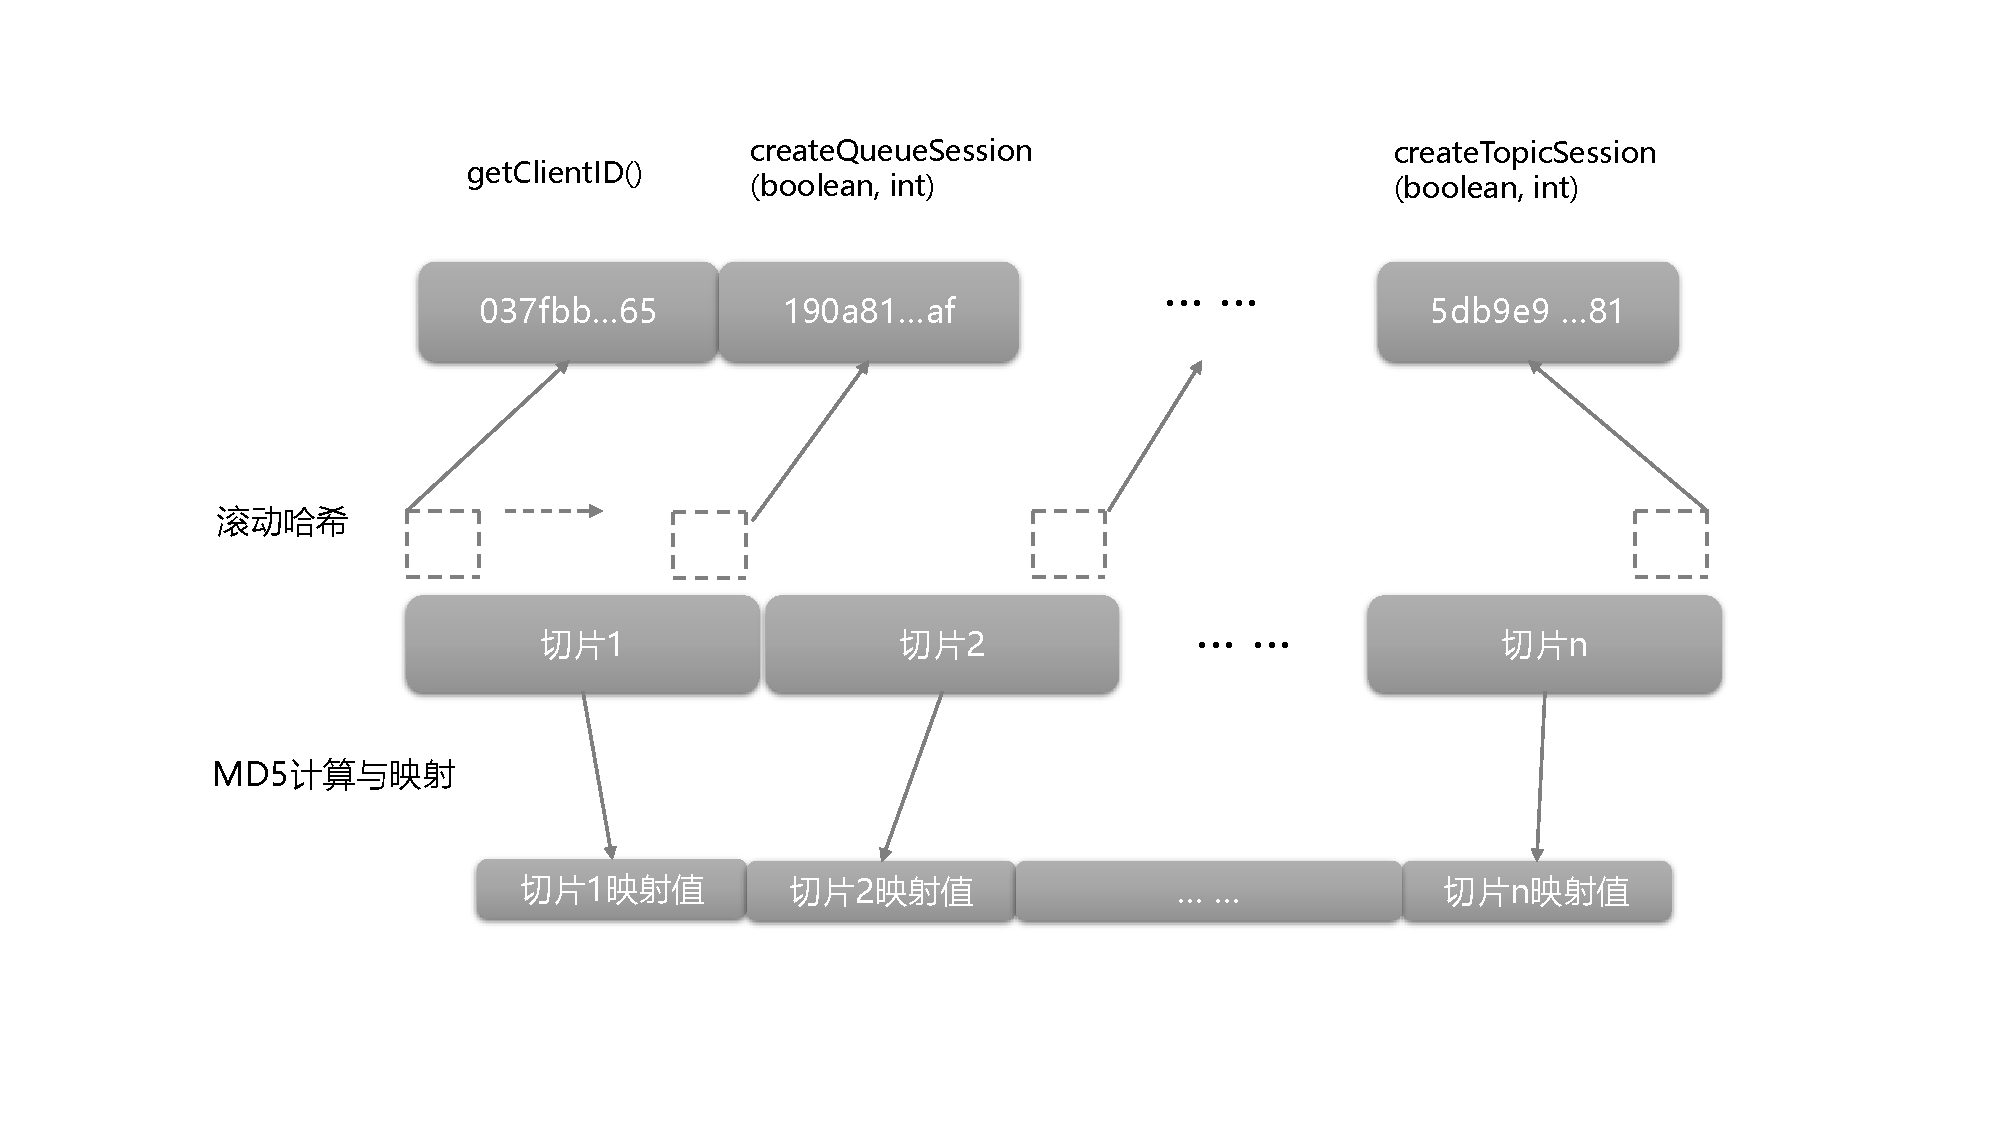
\includegraphics[width=15cm]{fuzzy.pdf} \\
  \caption{使用特征提取器从字节码文件中获取特征并存储为树型数据结构}
 \label{fig:fuzzy}
\end{figure}



\begin{table}[!hpt]
  \caption{标准库org.codehaus.activemq中的两个类包含方法(部分)的情况}
  \label{tab:activemq}
  \centering
  \begin{tabular}{cc} \toprule
%    \multicolumn{2}{c}{Item} \\ \cmidrule(r){1-2}
    方法 & org.codehaus.activemq.ActiveMQConnection\$createSession  \\ \midrule
    描述符特征 & public javax.jms.Session(boolean, int)  \\ 
    字节码指令序列 & 2a b6 2a b6 bb 59 2a 1b 99 03 a7 1c b7 b0 \\
    粗粒度特征 & d8a58a75cf9b3272e8736cd74256fdc7 \\
    细粒度特征 &  45422e23d690d166bc6dd144f226076f \\ \bottomrule
  \end{tabular}
\end{table}


\begin{algorithm}[htb]
  \caption{类的模糊哈希值计算}
  \label{algo:fuzzyhash}
  \small
  \SetAlgoLined
  \KwData{类节点cNode}
  \KwResult{类的模糊哈希值Fuzzy\_hash }

  initialization\;
  sort(cNode.getMethods())\;
  Sequence$\leftarrow$null\;
  \For{mNode $\in$ cNode.getMethods()}{Sequence $\leftarrow$ Sequence $cascade$ mNode.getFeature()\;}
  Slices$\leftarrow$rolling\_hash(Sequence)\;
  Fuzzy\_hash$\leftarrow$null\;
  \For {slice $\in$ Slices}{F\_hash\_slice$\leftarrow$mapping\_function(MD5(slice))\;
  					 Fuzzy\_hash$\leftarrow$Fuzzy\_hash $cascade$ F\_hash\_slice\;}

\end{algorithm}


\subsubsection{包层}

包实现为\textit{pNode}(Package Node)类,是一个特征树的根节点。包层不产生特征,用于管理属于该包下的各个类。为了解决APK产生的包中可能存在目录结构的混淆问题,每一个包都采用根包作为唯一的根节点,其下包含的子包以及子包中的二级子包等所拥有的类都归为根包的类。

最后将从包到方法的各个节点封装为一个\textit{javaTree}类,负责统筹管理从文件的筛选到各级节点的生成等诸多工作。



\section{特征存储}

为了便于特征的查找与管理,我将哈希树输出的特征存放在MySQL数据库中,步骤如下:

\begin{enumerate}
\item{设计数据库scheme:tpl如表\ref{tab:mysql}所示,在tpl下创建表maven,存储从Maven仓库获取的标准库。}
\item{遍历本地爬取到的Maven仓库,当文件夹中包含\textit{META-INF}时表明当前目录为一个根包的目录。}
\item{在根包的目录上构建哈希树,解析目录中的文件,形成该包下各类、各方法的特征。}
\item{用插入语句将特征存储到数据库中}
\end{enumerate}

\begin{table}[!hpt]
  \caption{MySQL数据库中tpl的scheme}
  \label{tab:mysql}
  \centering
  \begin{tabular}{l|lllll} \toprule
%    \multicolumn{2}{c}{Item} \\ \cmidrule(r){1-2}
    字段 &  package & class & method & coarse feature & fine feature \\ \midrule
    数据类型 & varchar(255) & varchar(255) & varchar(1024) & varchar(255) & varchar(255)  \\  \bottomrule

  \end{tabular}
\end{table}



\section{特征匹配}


\begin{table}[!hpt]
  \caption{标准库与安卓应用的相关符号及说明}
  \label{tab:symbol}
  \centering
  \begin{tabular}{cc} \toprule
%    \multicolumn{2}{c}{Item} \\ \cmidrule(r){1-2}
    符号 &  说明 \\ \midrule
    $T_{sim}$ & 相似度阈值,相似度超过此值的两个特征认为互相匹配 \\
	$feature_{lib}$ & 来源于标准库的一个类或者方法的特征 \\ 
	$feature_{app}$ & 来源于安卓应用的一个类或者方法的特征 \\
	$C_{lib}$ & 标准库所包含的类的集合 \\
	$C_{app}$ & 安卓应用所包含的类的集合 \\
	$M_{class}$ & 类所包含的方法的集合\\
	$Similarity_p$ & 两个包之间的相似度\\
	$Similarity_c$ & 两个类之间的相似度\\
	 \bottomrule

  \end{tabular}
\end{table}


\subsubsection{相似度}

为了表征标准库与来自Apk的包的相似程度,我引入了相似度来量化这一概念。相似度适用于不同来源(Maven/APP)的类或方法的匹配,是一个介于0和1之间的数,1表示完全匹配。若要判断APP所包含的包是否存在于数据库中,需要查看数据库中是否存在足够数量的类,使得这些类的特征值与APP中类的特征值的相似度都超过了一定阈值。由于类的特征值是根据方法的特征值生成的,因此类的相似程度能过说明其内各个方法的相似程度。类和方法的特征均为字符串序列表示的哈希值,因此用编辑距离来计算两个序列之间的相似度:
\begin{equation}
Similarity(feature_{lib},feature_{app})=\frac{edit\_distance(feature_{lib},feature_{app})}{max\{length(feature_{lib}),length(feature_{app})\}}
\end{equation}

对于待定的阈值$T_{sim}$,定义来自标准库的特征$feature_{lib}$与来自APP的特征$feature_{app}$匹配,如果满足:

\begin{equation}
Similarity(feature_{lib},feature{app})\ge T_{sim}
\end{equation}


同时,标准库的规模也应该纳入考虑范畴。一些大规模的类、或者相似的类,可能在部分方法上有相似之处,在实现逻辑上有相同点,因此不能仅仅因为成功匹配其下的一部分类就将其所谓候选库。而一些小规模的类,方法数可能很少,一定数量的类匹配就说明其有很大概率就是APP所使用到的库。一种简明的相似度计算方法如下:
\begin{equation}
Similarity_p(lib,app)=\frac{|\{c_1,c_2,\dots ,c_n\}|}{|C_{lib}|} \in [0,1]
\end{equation}

其中,$c_i$满足:
\begin{subequations}
\begin{align}
(a)&\ c_i \in C_{lib}\\
(b)&\ \exists\  c'\in C_{app},Similarity(c_i,c')\ge T_{sim}
\end{align}
\end{subequations}


类似地,用$Similarity_c$表示方法相似度,也可以在方法粒度上实现更为精确的匹配:
\begin{equation}
Similarity_c(class_{lib},calss_{app})=\frac{|\{m_1,m_2,\dots ,m_n\}|}{|M_{class_{lib}}|} \in [0,1]
\end{equation}

其中,$m_i$满足:
\begin{subequations}
\begin{align}
(a)&\ m_i \in M_{class_{lib}}\\
(b)&\ \exists\  c'\in M_{class_{app}},Similarity(m_i,m')\ge T_{sim}'
\end{align}
\end{subequations}



\subsubsection{匹配策略}

来自Maven中央仓库的标准库数量巨大,一个包中可能包含多个子包,包的版本数可能超过50个。一种朴素的匹配方法是:将来自Maven的标准库与来自App的包两两匹配,计算其下类的相似度,但这会产生以亿为单位的配对数,耗时严重。因此我引入了如图\ref{fig:match}所示的两种策略来加速匹配的过程,分别是两级特征与优先级队列。

\begin{figure}[!htp]
  \centering
  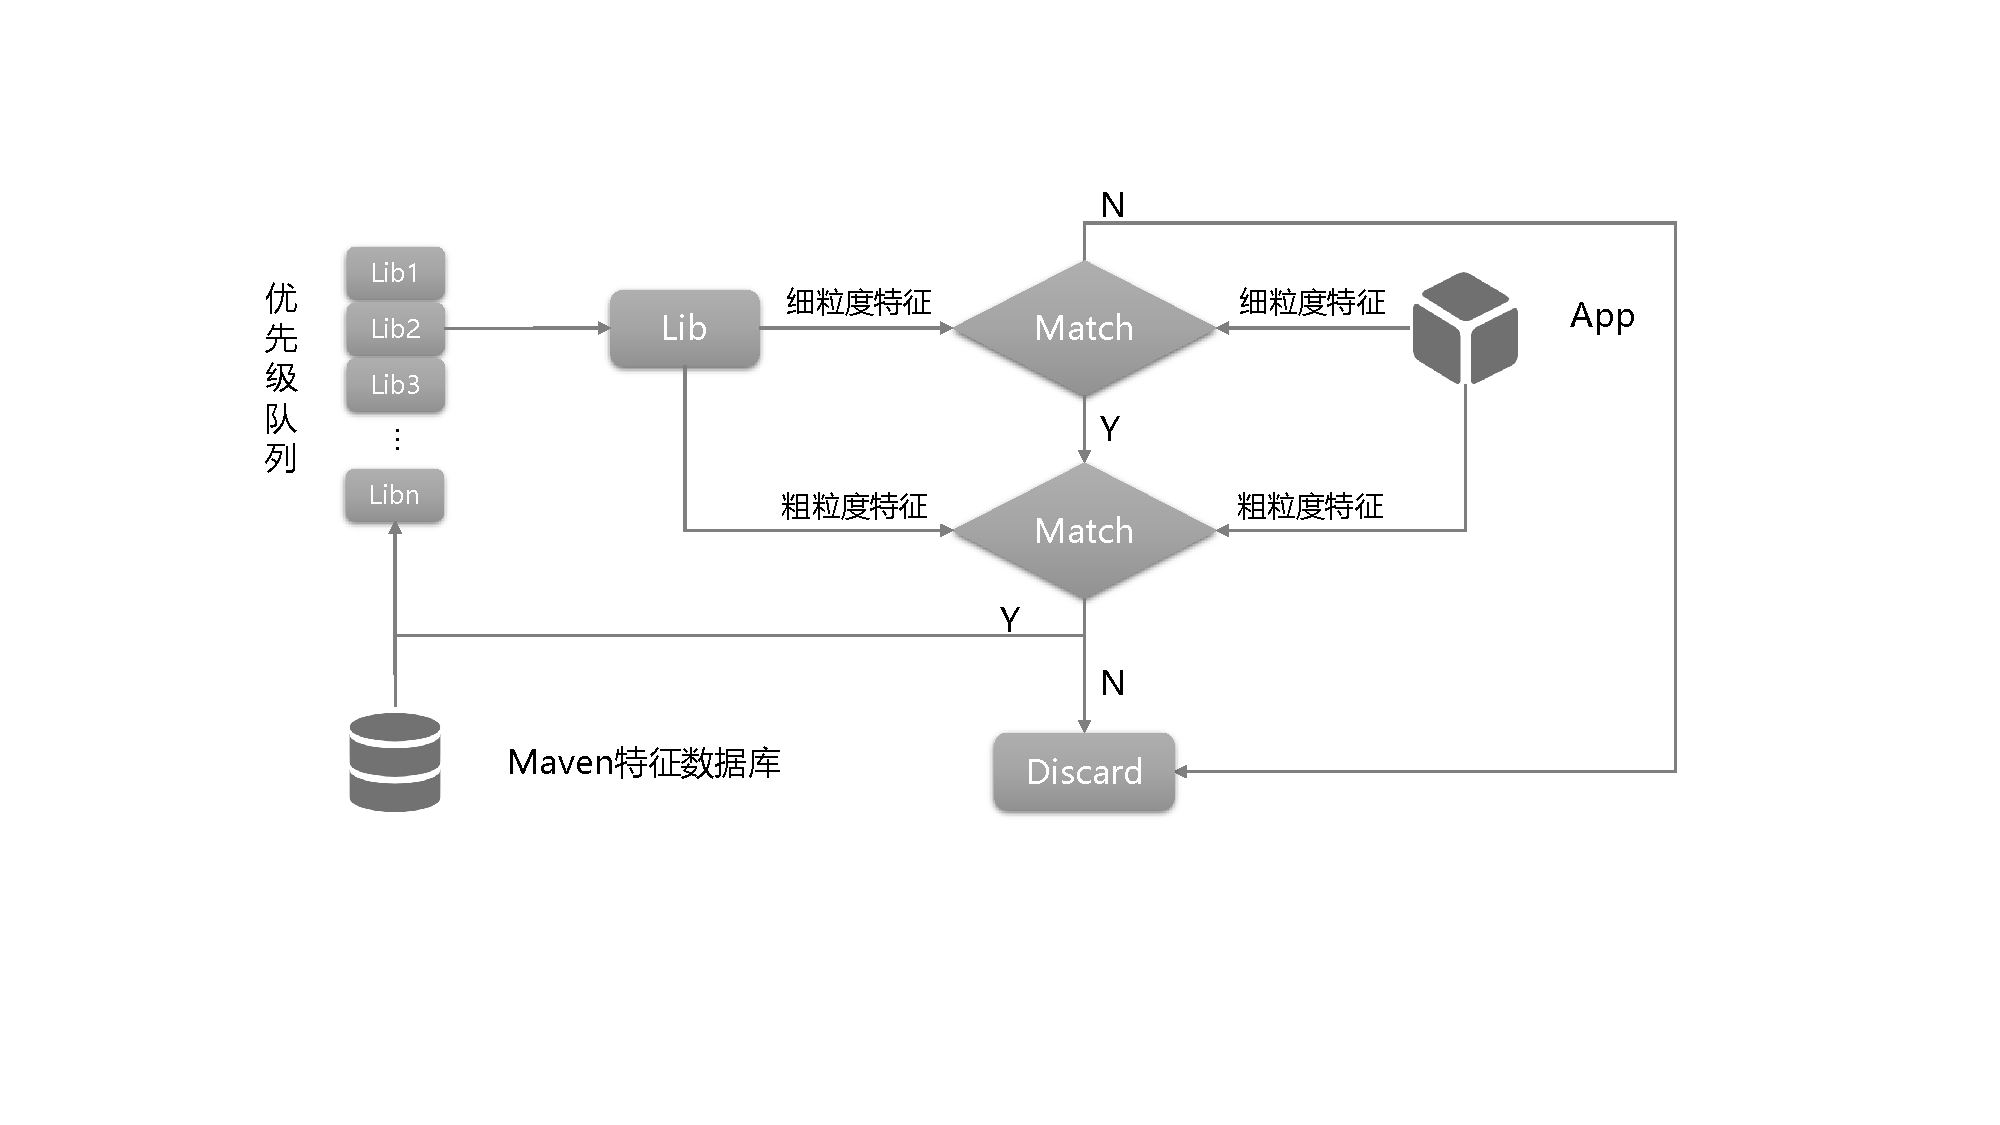
\includegraphics[width=15cm]{match.pdf} \\
  \caption{数据库匹配的两种加速策略——两级特征与优先级队列}
 \label{fig:match}
\end{figure}


\paragraph{两级特征策略}包含粗粒度、细粒度两种计算方法复杂度不同、精确度不同的特征,思想为首先利用粗粒度特征初步缩小匹配范围,即App中使用到了Maven的哪些标准库,再用细粒度特征确定这些库的具体版本。一个库如果没有通过粗粒度筛选,说明其方法的数量、各方法的参数数量、返回值及参数的类型这些特征与App存在较大差异,因此它几乎不可能在App中使用到,对这样的库进行具体版本的匹配也是没有意义的。对于通过粗粒度筛选的库,说明它在方法层面与App中的包有一定相似程度,此时再通过基于字节码生成的细粒度特征来精准匹配,不同版本所带来的细微差异也能够体现在特征中。

\paragraph{优先级队列策略}基于一个“局部性”假设:{\kaishu 前一个来自App的类匹配完毕时,新到来的类有较大可能与前一个类处于同一个包中}。


这一假设在直观上是合理的,因为在匹配的过程中,我按照App目录中的文件顺序进行处理,相邻的类处于同一个目录下。尽管App可能经过了目录结构的混淆处理,即将来自不同包的类混入到一个目录下,但除非所有的包都做了混淆且每一个类都被单独打乱路径而非以多个类为批次操作,否则此假设在大多数情况下都成立。


为了充分利用这一假设,对待匹配的App设置一个优先级队列。初始时优先级队列为空,从数据库中按序取出$K$个类的记录加入到队列当中。队列中元素的优先级$Priority$定义为与当前待匹配App的类的相似度,其中细粒度特征的相似程度由于包含了更多的原始信息而被赋予更大的权重:

\begin{equation}
\begin{aligned}
Priority(c_{lib},c_{app})&=0.3\times Similarity(feature^{coarse}_{c_{lib}},feature^{coarse}_{c_{app}})\\
						 &+0.7\times Similarity(feature^{fine}_{c_{lib}},feature^{fine}_{c_{app}}),\\
						 &\ \ c_{lib}\in C_{lib}, c_{app}\in C_{app}
\end{aligned}
\end{equation}


在进行匹配时,依次将优先级队列中的记录取出,计算与待匹配类的相似度,进一步计算优先级,按照优先级从大到小重排队列。
队列中的记录全部使用完毕后,从数据库中取出一条新的记录,计算相似度与优先级,并插入到队列的合适位置,如果优先级小于队列尾部记录的优先级则不进入队列。以此类推,将数据库中的所有记录进行匹配。当前待测类匹配流程完毕后,从App中取出下一个待测类,首先与优先级队列中的记录匹配,队列匹配完毕后再从数据库中取得记录,按照此方法将App中的所有类进行匹配。

对于某次匹配结果:
\begin{enumerate}
\item{如果完全匹配,即相似度为1,则中止当前流程,直接记录此类属于数据库中类所在的标准库。}
\item{如果相似度小于1,则以优先级队列中优先级最高的记录为最佳匹配,并将该记录来自的标准库作为当前待测类的识别结果。}
\end{enumerate}


具体匹配算法如\ref{algo:match}所示,1-2行首先初始化一个优先级队列和空的映射关系字典;第3行遍历待测App的类集合中的每一个类;第4-13行进入优先级队列为空的情况,第5-7依次从标准库的类的集合中取出类,计算它与当前App的类的匹配优先级,根据结果加入到优先级队列中,第8-13行在完全匹配发生时提前中止循环;第14-31行处理优先级队列非空的情况,其中第15-22行表明匹配时首先从优先级队列中取出元素,23-31行为从数据库中取出元素参与匹配;33行将每个类的最佳匹配作为它的最终匹配结果;34行将匹配结果存储到映射关系字典中。


\begin{algorithm}[htb]
  \caption{标准库与App的匹配算法}
  \label{algo:match}
  \small
  \SetAlgoLined
  \KwData{标准库特征数据库$C_{lib}$,App特征数据库$C_{app}$}
  \KwResult{匹配结果$Package$}

  Initialize priority queue $Queue_{p}$\;
  Initialize mapping relation $Package\leftarrow empty\ dictionary$\;
  \For{$c_{app} \in C_{app}$}{
	\eIf{$isEmpty(Queue_{p})$}{
		\For{$c_{lib} \in C_{lib}$}{
			$priority \leftarrow Priority(c_{lib},c_{app})$\;
			$Queue_p\dot enQueue(c_{lib},priority)$\;
			\eIf{priority=1}{$break\;$}{$continue$\;}
		}
	}
	{
		\For{$c_{lib} \in Queue_p$}{
			$priority \leftarrow Priority(c_{lib},c_{app})$\;
			\eIf{priority=1}{$break\;$}{$continue$\;}
		}
		\For{$c_{lib} \in C_{lib}$}{
			$priority \leftarrow Priority(c_{lib},c_{app})$\;
			$Queue_p.enQueue(c_{lib},priority)$\;
			\eIf{priority=1}{$break\;$}{$continue$\;}
		}
	}
	$c_{lib}^{match}\leftarrow Queue_p.first()$\;
	$Package[c_{app}]\leftarrow c_{lib}^{match}.get\_package()$\;
  }
\end{algorithm}


\section{本章小节}
本章详细介绍了TPL-V Detector的设计细节。3.1节概括了TPL-V Detector的整体架构以及设计思路,包括了预处理、特征树构建、特征存储与匹配三个模块。3.2节介绍了包的预处理流程,包括jar包与apk安装包的解压缩、dex文件到class文件以及class文件到字节码文件的转换。3.3节从方法、类、包三个层次叙述了特征树的构建,引入了两级特征的机制,并说明了两级特征的作用与生成方法。3.3节简单说明了如何用数据库存储特征以及表的设计模式。3.4节详细介绍了特征匹配使用的策略,包含相似度的计算方法、两级特征匹配策略和优先级队列匹配策略,并用伪代码具体叙述了匹配算法的整个流程。综上所述,TPL-V Detector是一个基于先验知识的、抗混淆的、第三方库及其具体版本检测系统,通过构建特征树的方法进行标准库与混淆库的匹配,同时引入了两级特征和优先级队列匹配策略来检测具体版本以及加速匹配过程。


\chapter{混淆第三方库检测实验}



\section{系统实现与实验概述}

\subsection{系统实现}
TPL-V Detector系统的控制流程部分用Python实现,负责jar包、apk等文件的处理,调用命令行工具javap对class文件进行反编译,以及对字节码文件的筛选。特征树的构建用C++实现,负责从字节码中提取特征,建立树状数据结构,以及生成各类的特征。其中Python通过pymsql库连接MySQL数据库,实现特征的存储和管理、特征的查询与匹配。系统实现包含脚本文件共19个,代码行数约2500行。其他配置见表\ref{tab:config}。

\begin{table}[!hpt]
  \caption{系统实现与实验环境配置}
  \label{tab:config}
  \centering
  \begin{tabular}{cc} \toprule
%    \multicolumn{2}{c}{Item} \\ \cmidrule(r){1-2}
    配置 &  详情 \\ \midrule
	CPU & Intel(R) E5-2630 v4\\
	OS & Ubuntu 16.04.5 LTS\\
	Core & 8\\
	Python & 3.6.5\\
	GCC & 5.4.0\\
	MySQL & 8.0.29\\
	Memory & 8GB\\
	 \bottomrule

  \end{tabular}
\end{table}


\subsection{实验流程}
实验所用数据集包含了6个来自Maven的标准库,共40个版本,以及10款来自第三方市场的App。实验首先在SDK数据集上进行,测试类的相似度阈值的最佳取值,然后使用混淆工具Proguard对Maven标准库进行混淆,将混淆前的标准库和经过混淆的标准库分别交由TPL-V Detector系统处理和存储,以未混淆的标准库作为先验知识,检测混淆过后的标准库,最后对其各项指标进行评估。接下来在真实数据上即来自第三方市场的App上进行实验,首先获取App中包含的第三方库,作为先验知识数据库,随后由TPL-V Detector进行检测,将结果与实际情况进行对比,评估其准确率及其它指标。此外,本文还将系统与现有的一些其他检测方法在准确率和耗时上进行了对比,以分析系统的优越性与不足之处。

\subsection{评价指标}
系统评价指标包括准确率(Accuracy)、精确率(Precision)、召回率(Recall)、F1得分(F1\ score)和误报率(FPR),各自定义如下:

\begin{subequations}
\begin{align}
Accuracy&=\frac{TP+TN}{TP+TN+FP+FN}\\
Precision&=\frac{TP}{TP+FP}\\
Recall&=\frac{TP}{TP+FN}\\
F1\_score&=\frac{2\times Precision\times Recall}{Precision+Recall}\\
FPR&=\frac{FP}{FP+TN}
\end{align}
\end{subequations}

其中TP、FP、TN、FN分别代表检测结果中真阳性、假阳性、真阴性、假阴性的数量。


\section{混淆SDK检测实验}

\subsection{Maven数据集}
Maven仓库未Java开发者提供了丰富的开源组件,是目前最流行的开源软件包生态系统之一。本文从Maven中央仓库中选取了6个开源标准库,各库及其版本情况如表\ref{tab:maven}所示。

\begin{table}[!hpt]
  \caption{实验所选Maven标准库及其版本数}
  \label{tab:config}
  \centering
  \begin{tabular}{cc} \toprule
%    \multicolumn{2}{c}{Item} \\ \cmidrule(r){1-2}
    库 &  版本数 \\ \midrule
	net.sf.ezmorph & 11\\
	com.alibaba.fastjson & 15\\
	com.github.xujiaji.happy-bubble & 2\\
	com.squareup.okhttp3.okhttp & 42\\
	com.squareup.okio & 20\\
	com.tencent.mm.opensdk & 2\\
	 \bottomrule

  \end{tabular}
\end{table}

\subsection{阈值$T_c$的选取}
阈值$T_c$用于判断两个类是否匹配,如果类$class_a$和类$class_b$满足特征的相似度超过阈值,定义两者具有匹配关系$match$,即:
\begin{equation}
\begin{aligned}
class_a\ &match\ class_b,\\
if\ similarity(class_a,class_b)&=1-\frac{edit\_distance(feature_{a},feature_{b}}{length(feature_a)+length(feature_b)}\\
&> T_c
\end{aligned}
\end{equation}

阈值$T_c$的选取非常关键,对实验结果影响较大。阈值过高会导致匹配对细微的差异过于敏感,导致准确率降低;阈值过低会导致匹配门槛过于宽松,准确率虽然有所升高,但是误报率也会相应升高。因此本文对随机字符串的编辑距离,即Levenshtein距离的分布情况进行了描绘以确定合适的阈值选取范围。对于所含字符随机、长度随机的1000个字符串,分成500对分别计算其Levenshtein距离,进一步按照本文方法计算相似度得分,并将[0,1)平均分为10个区间,统计落入各区间的字符串对的数量。

\begin{figure}[!htp]
  \centering
  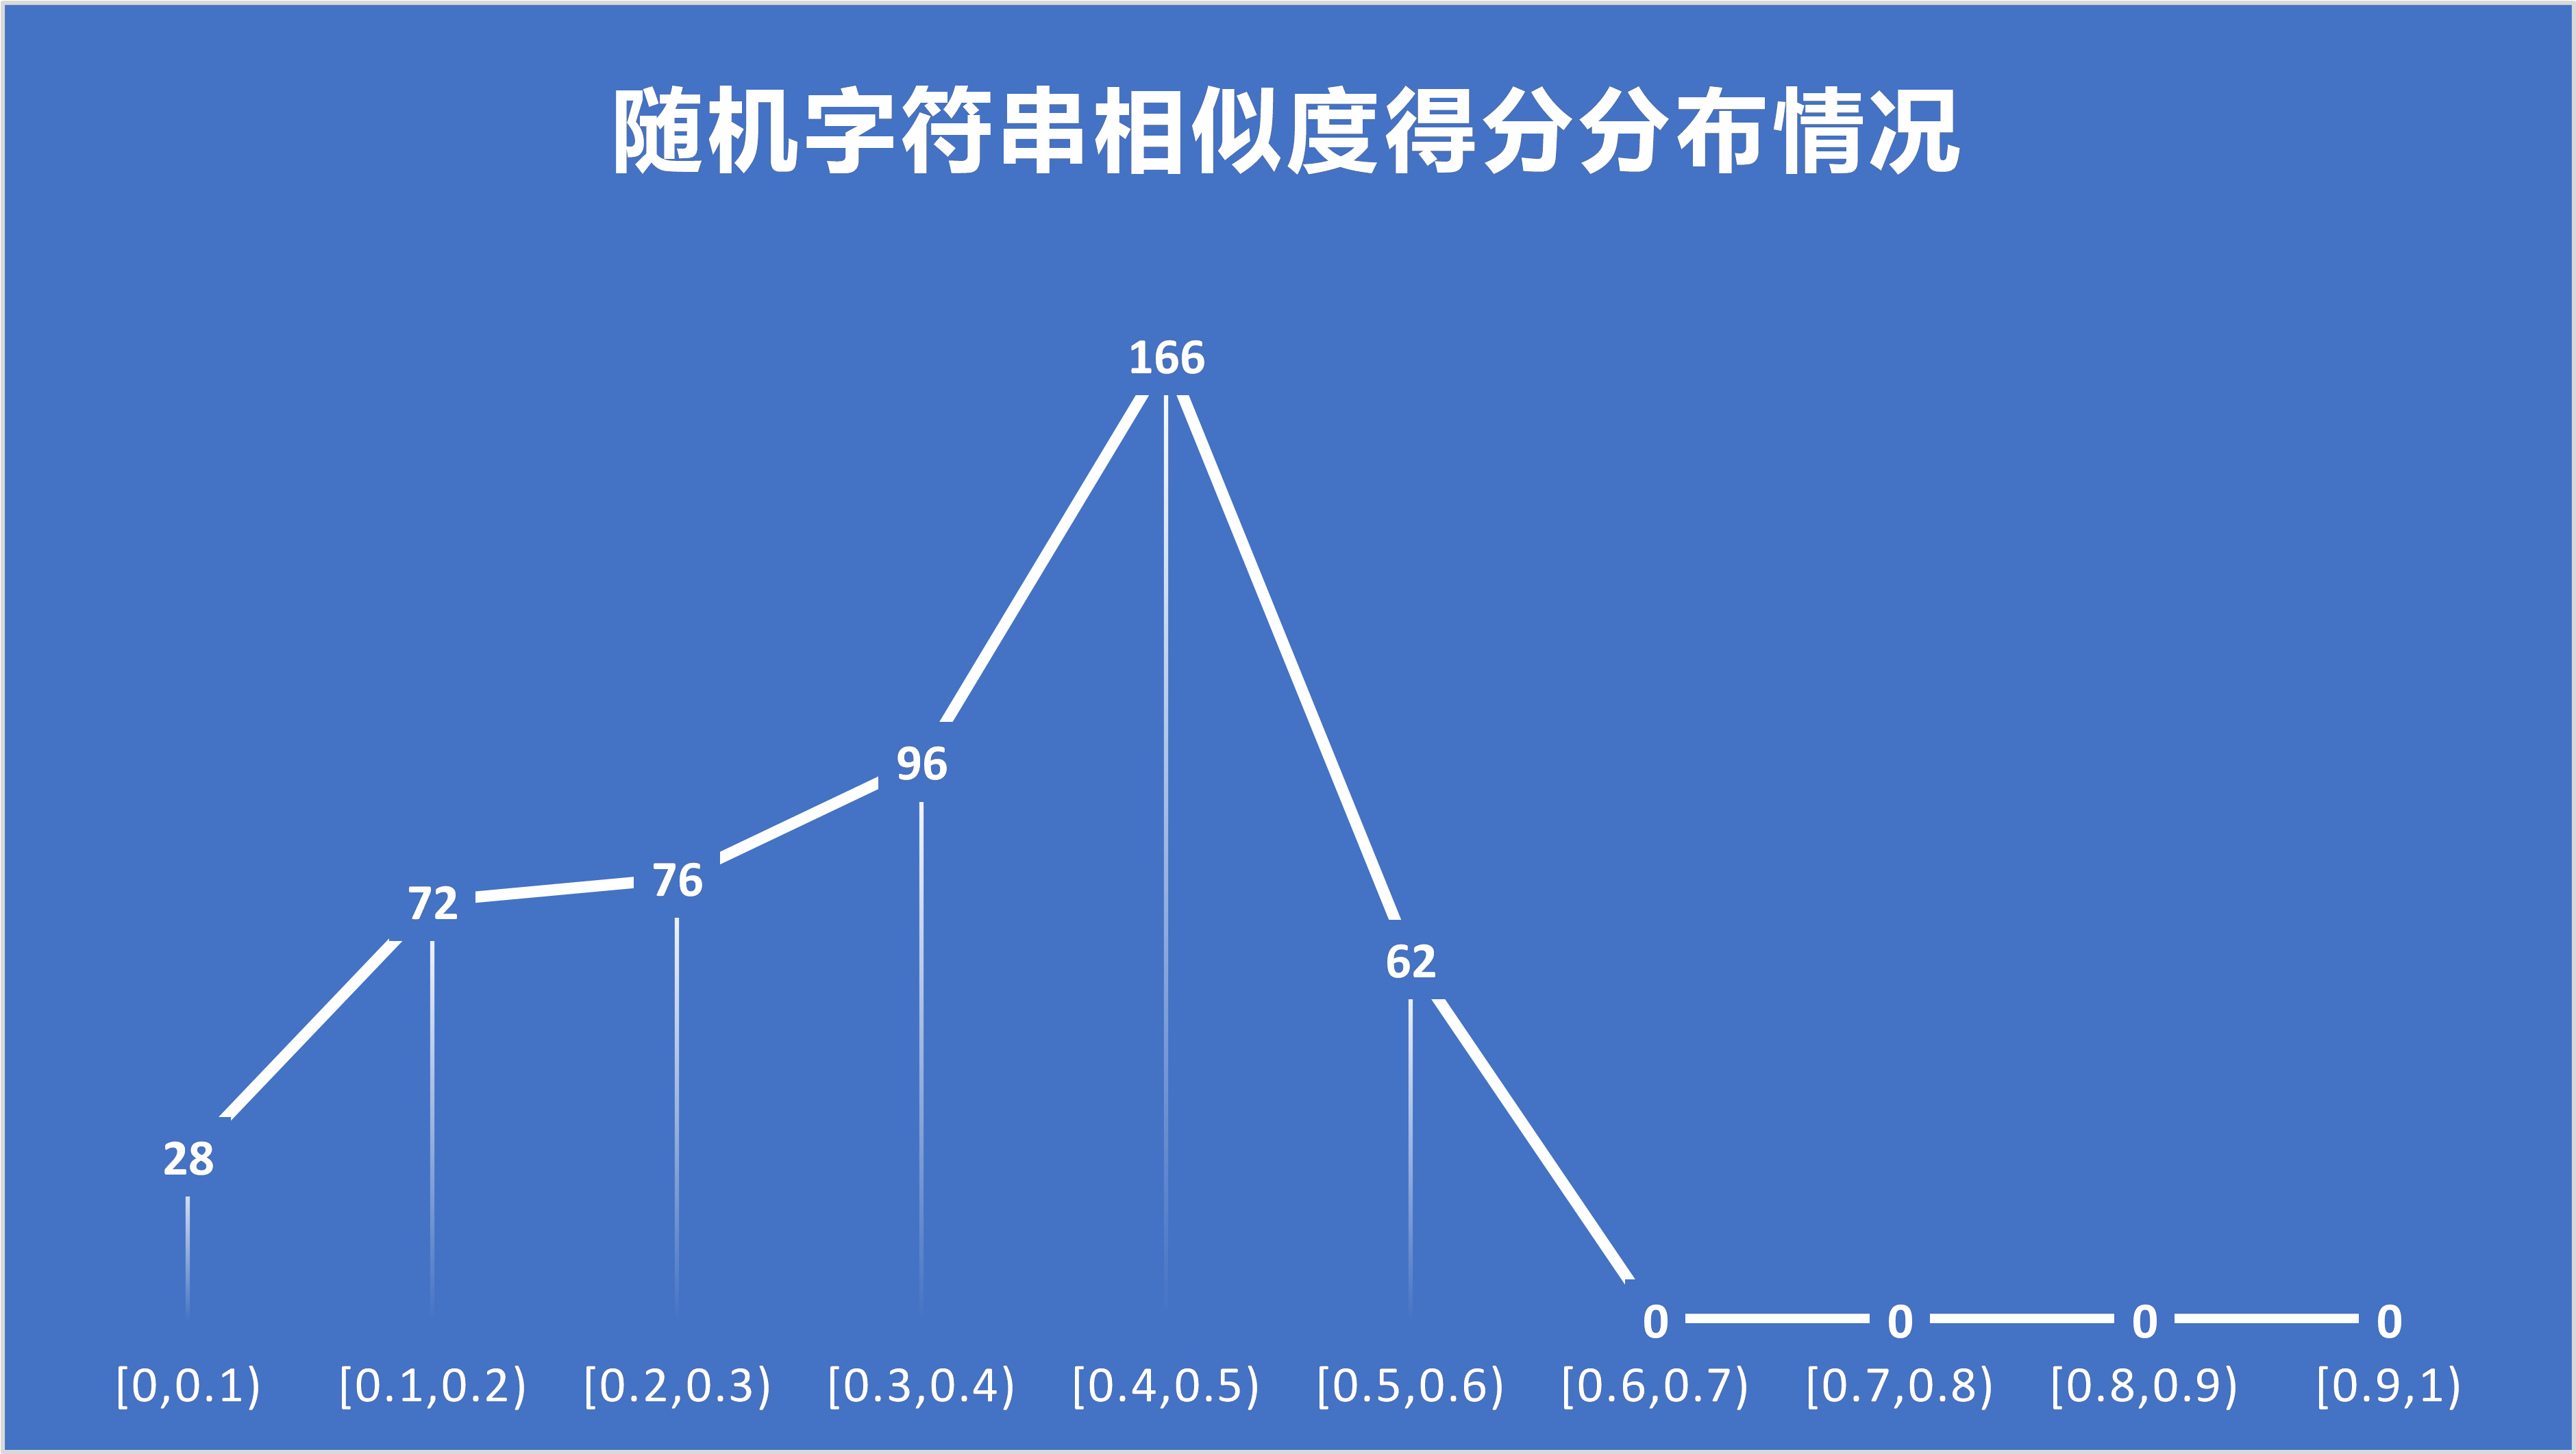
\includegraphics[width=12cm]{dist.png} \\
  \caption{随机生成的字符串的相似度得分分布情况}
 \label{fig:distribution}
\end{figure}


结果的分布情况如图\ref{fig:distribution}所示。根据图片可以看出,完全随机的两个字符串的相似度得分超过0.6的概率很小,因此选择$T_c=0.6$,以将尽可能多的库识别出来。

\subsection{TPL-V Detector性能评估}

\subsubsection{粗粒度-库匹配}
实验所选的六个库的各版本数之和为92,即数据库中包含了92个独立的库。根据两级特征匹配策略,首先使用粗粒度特征来识别混淆的六个库分别对应与哪一个标准库。将混淆库从1至6依次编号,对于一个混淆库(例如混淆库1)与未混淆库(例如com.squareup.okio),首先将其下的类进行两两匹配,计算每一个配对的相似度得分。包含方法数多的类的匹配难度更高,对与不包含方法的类,其特征值是空字符串生成的哈希值,可以与任意另一个方法数为0的类匹配。即便在最初特征生成的过程中,TPL-V Detector将文件大小不超过1KB的字节码文件删去,但上面的极端情况仍然可以表明方法数不同的类的匹配难度不同,因此引入方法数占总方法数的比例作为该类的权重,即相似度得分前的系数项。

\begin{algorithm}[htb]
  \caption{粗粒度匹配实验算法}
  \label{algo:coarse_exp}
  \small
  \SetAlgoLined
  \KwData{未混淆的标准库集合$L$,混淆后的标准库$L^{obfus}$}
  \KwResult{混淆库与未混淆库映射关系$obfus\_from$}

  Initialize obfuscated libraries $C_{lib}^{obfus}$\;
  Initialize score list $score\_list\leftarrow \ empty\ list$\;
  \For{$l^{obfus} \in L^{obfus}$}{
	Initialize $score\_list[l^{obfus}]\leftarrow\ empty\ dictionary$\;
	\For{$l \in L$}{
		$score(l^{obfus},l)\leftarrow 0$\;
		\For{$c^{obfus} \in C_{l^{obfus}}$}{
			\For{$c \in C_{l}$}{
				\eIf{$c^{obfus}\ match\ c$}{
					$score\leftarrow score+similarity(c,c^{obfus})\times \frac{|c.get\_methods()|}{|l.get\_methods()|}$\;
				}
				{
					continue\;
				}
			}
		}
		$score\_list[l^{obfus}]\leftarrow score\_list[l^{obfus}]\cup \{<l,score>\}$\;
	}
	$obfus\_from[l^{obfus}]\leftarrow l,max\{score\}\ for\ <l,score>\in score\_list[l^{obfus}]$\;
  }
\end{algorithm}


具体算法如\ref{algo:coarse_exp}所示,对每一个混淆库,计算其与6个未混淆库的得分,选择得分最高者作为它对应的标准库,实验结果表\ref{tab:coarse_sdk},加粗的单元格表示所在行列对应的混淆库与未混淆库匹配。


\begin{table}[!hpt]
  \caption{标准库混淆前后在粗粒度特征上的匹配结果}
  \label{tab:coarse_sdk}
  \centering
  \begin{tabular}{ccccccc} \toprule
%    \multicolumn{2}{c}{Item} \\ \cmidrule(r){1-2}
      & 混淆库1 &  混淆库2 & 混淆库3 & 混淆库4 & 混淆库5 & 混淆库6 \\ \midrule
	ezmorph\tnote{a} & \textbf{0.930}\tnote{b} & 0.493 & 0.465 & 0.518 & 0.494 & 0.462\\
	fastjson & 0.377 & 0.446 & \textbf{0.852} & 0.397 & 0.446 & 0.463 \\
	happy-bubble & 0.529 & 0.486 & 0.486 & \textbf{0.929} & 0.500 & 0.486 \\
	okhttp & 0.388 & 0.444 & 0.442 & 0.379 & 0.426 & \textbf{0.808}\\
	okio & 0.400 & \textbf{0.842} & 0.527 & 0.420 & 0.439 & 0.473\\
	opensdk & 0.414 & 0.456 & 0.491 & 0.435 & \textbf{0.842} & 0.455\\
	 \bottomrule

  \end{tabular}
    \begin{tablenotes}
    \item [a] 为表示方便省略标准库的groupID。% or \item [a]
    \item [b] 粗体数据表示该数据为所在行/列中的最大值。% or \item [b]
    \end{tablenotes}
\end{table}

根据表\ref{tab:coarse_sdk},混淆库从1至6分别对应于ezmorph、okio、fastjson、happy-bubble、opensdk、okhttp,与实际上混淆的对应关系相同,混淆的第三发放标准库被全部检测出来。


\subsubsection{细粒度-库匹配}

在确定了各混淆库对应的标准库后,需要使用基于字节码的细粒度特征确定具体版本。实验算法基本与算法\ref{algo:coarse_exp}相同,对于两个库,计算各个类的配对的相似度,以方法数为权重,计算两个库的总得分。对每个混淆库的得分列表,选取得分最高的未混淆库作为它的匹配结果。


各库版本匹配结果如图\ref{fig:version}所示,对每个库列出了排名前三的版本得分,由于opensdk和happy-bubble只包含两个版本,因此列出了前两名的版本得分。

\begin{figure}[!htp]
  \centering
  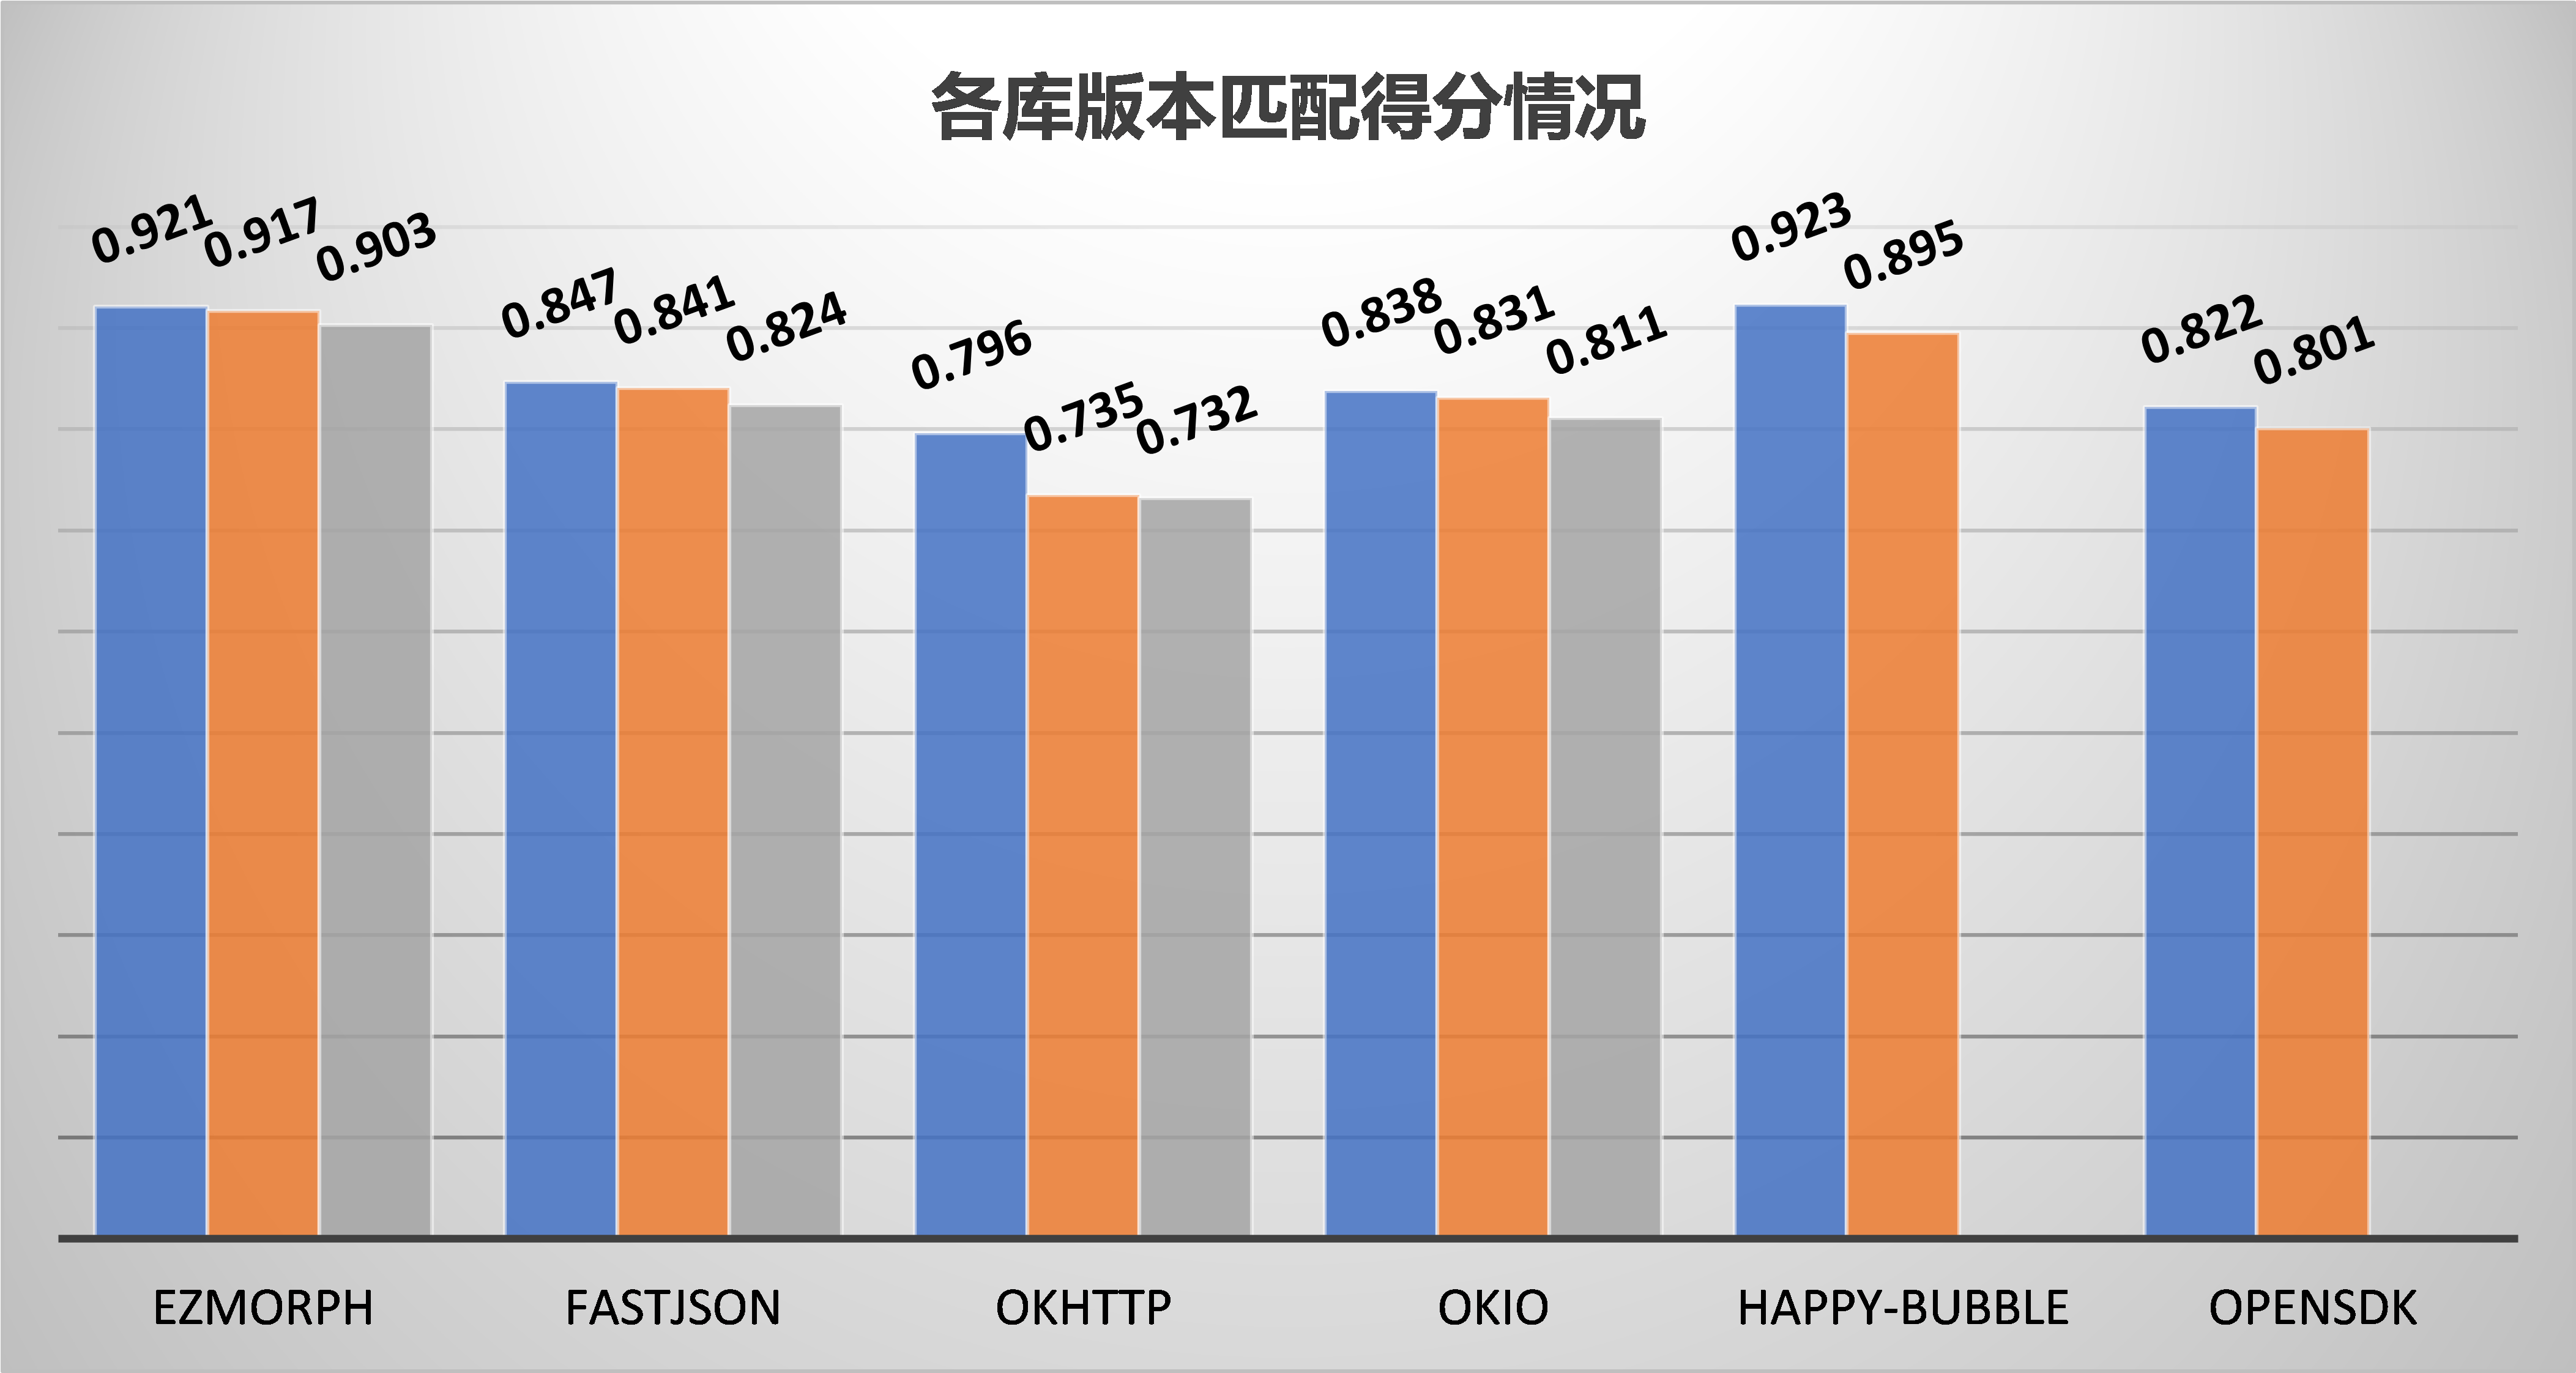
\includegraphics[width=12cm]{version.png} \\
  \caption{细粒度版本匹配各库的版本得分情况}
 \label{fig:version}
\end{figure}



\section{混淆安卓App第三方库检测实验}

\subsection{Android数据集}
Li\cite{li2021embedding}等人分析了大量的手机应用及其所使用的第三方库,本文从此数据集中选取了10款App作为实验的App数据集,并从这些App所包含的库中选择9个作为标准库数据集,各App编号及详情见附录A,包含情况如表\ref{tab:include}所示。

\begin{table}[!hpt]
  \caption{App对各标准库的包含情况}
  \label{tab:include}
  \centering
  \begin{tabular}{ccccccccccc} \toprule
%    \multicolumn{2}{c}{Item} \\ \cmidrule(r){1-2}
      \diagbox{Lib}{App}& 1 & 2 & 3 & 4 & 5 & 6 & 7 & 8 & 9 & 10 \\ \midrule
	Google Ads & \ding{51} & \ding{51} & \ding{51} & \ding{51} & \ding{51} & \ding{55} & \ding{51} & \ding{51} & \ding{51} & \ding{51}  \\
	Apache Http & \ding{51} & \ding{55} & \ding{51} & \ding{55} & \ding{55} & \ding{51} & \ding{51} & \ding{55} & \ding{55} & \ding{55} \\
	Firebasee & \ding{51} & \ding{51} & \ding{51} & \ding{55} & \ding{55} & \ding{55} & \ding{55} & \ding{55} & \ding{55} & \ding{55} \\
	Square Dagger & \ding{51} & \ding{55} & \ding{55} & \ding{51} & \ding{51} & \ding{55} & \ding{55} & \ding{55} & \ding{55} & \ding{55}\\
	ChartBoost & \ding{55} & \ding{55} & \ding{55} & \ding{51} & \ding{55} & \ding{55} & \ding{55} & \ding{51} & \ding{55} & \ding{55}\\
	JavaX Annotation & \ding{51} & \ding{55} & \ding{55} & \ding{55} & \ding{55} & \ding{55} & \ding{55} & \ding{55} & \ding{55} & \ding{55}\\
	OKHttp3.0 & \ding{51} & \ding{55} & \ding{55} & \ding{55} & \ding{55} & \ding{55} & \ding{55} & \ding{55} & \ding{55} & \ding{55}\\
	Tencent SDKs & \ding{55} & \ding{55} & \ding{55} & \ding{51} & \ding{55} & \ding{55} & \ding{55} & \ding{55} & \ding{55} & \ding{55}\\
	ksoap2 & \ding{55} & \ding{55} & \ding{55} & \ding{55} & \ding{55} & \ding{55} & \ding{55} & \ding{55} & \ding{55} & \ding{51}\\
	 \bottomrule
  \end{tabular}
    \begin{tablenotes}
    \item \quad \quad \quad \quad \ding{51}表示app包含库,\ding{55}表示app不包含库。% or \item [a]
    \end{tablenotes}
\end{table}


\subsection{TPL-V Detector性能评估}

\subsubsection{在评价指标上的表现}


对于表\ref{tab:include}中的标准库,将每个库的每个版本作为一个独立的库,共得到529个标准第三方库作为先验知识。对于十款待测App,如果App的某个目录满足以下两个条件:
\begin{enumerate}
\item{该目录下包含class文件}
\item{该目录的上级目录不包含class文件}
\end{enumerate}
则将该目录作为一个根包的目录。这样做的依据是:一个App所引入的第三方库的根包含有子包(文件夹)、根层调用子包的逻辑以及自身的部分代码实现,根包的上层目录作为组Id不包含实现代码,仅为了表明包的所属机构以及创造隔离的命名空间。


因此对于App中每个满足上述条件的目录,都以此目录为包的根目录构建特征树,生成特征。由于App经过混淆处理,可能包括代码优化、资源压缩、死代码删除等步骤,因此为防止因为细微差别导致结果出现错判,设置阈值得分$T$,对于一对分别来自标准库和App的包,如果相似度得分阈值超过$T$,则认为该App使用了此标准库。

对阈值从0.6到0.9,以0.05为间隔,刻画准确率与召回率变化曲线,来选择最佳的阈值。如图\ref{fig:threshold}所示,在0.6至0.8区间,随着阈值升高,匹配标准更加严格,准确率有所上升,但是出现某些App内的混淆库找不到对应的标准库的情况,因此召回率下降严重。当阈值跌过0.7时,准确率发生快速下降情况,导致这一情况产生的原因可能是阈值接近了两个不相关库就能达到的得分,大量版本错误的库甚至是不同的库进入到结果列表当中。为了在保持召回率不过低的情况下,尽量提高准确率,本文选择阈值$T=0.8$。

\begin{figure}[!htp]
  \centering
  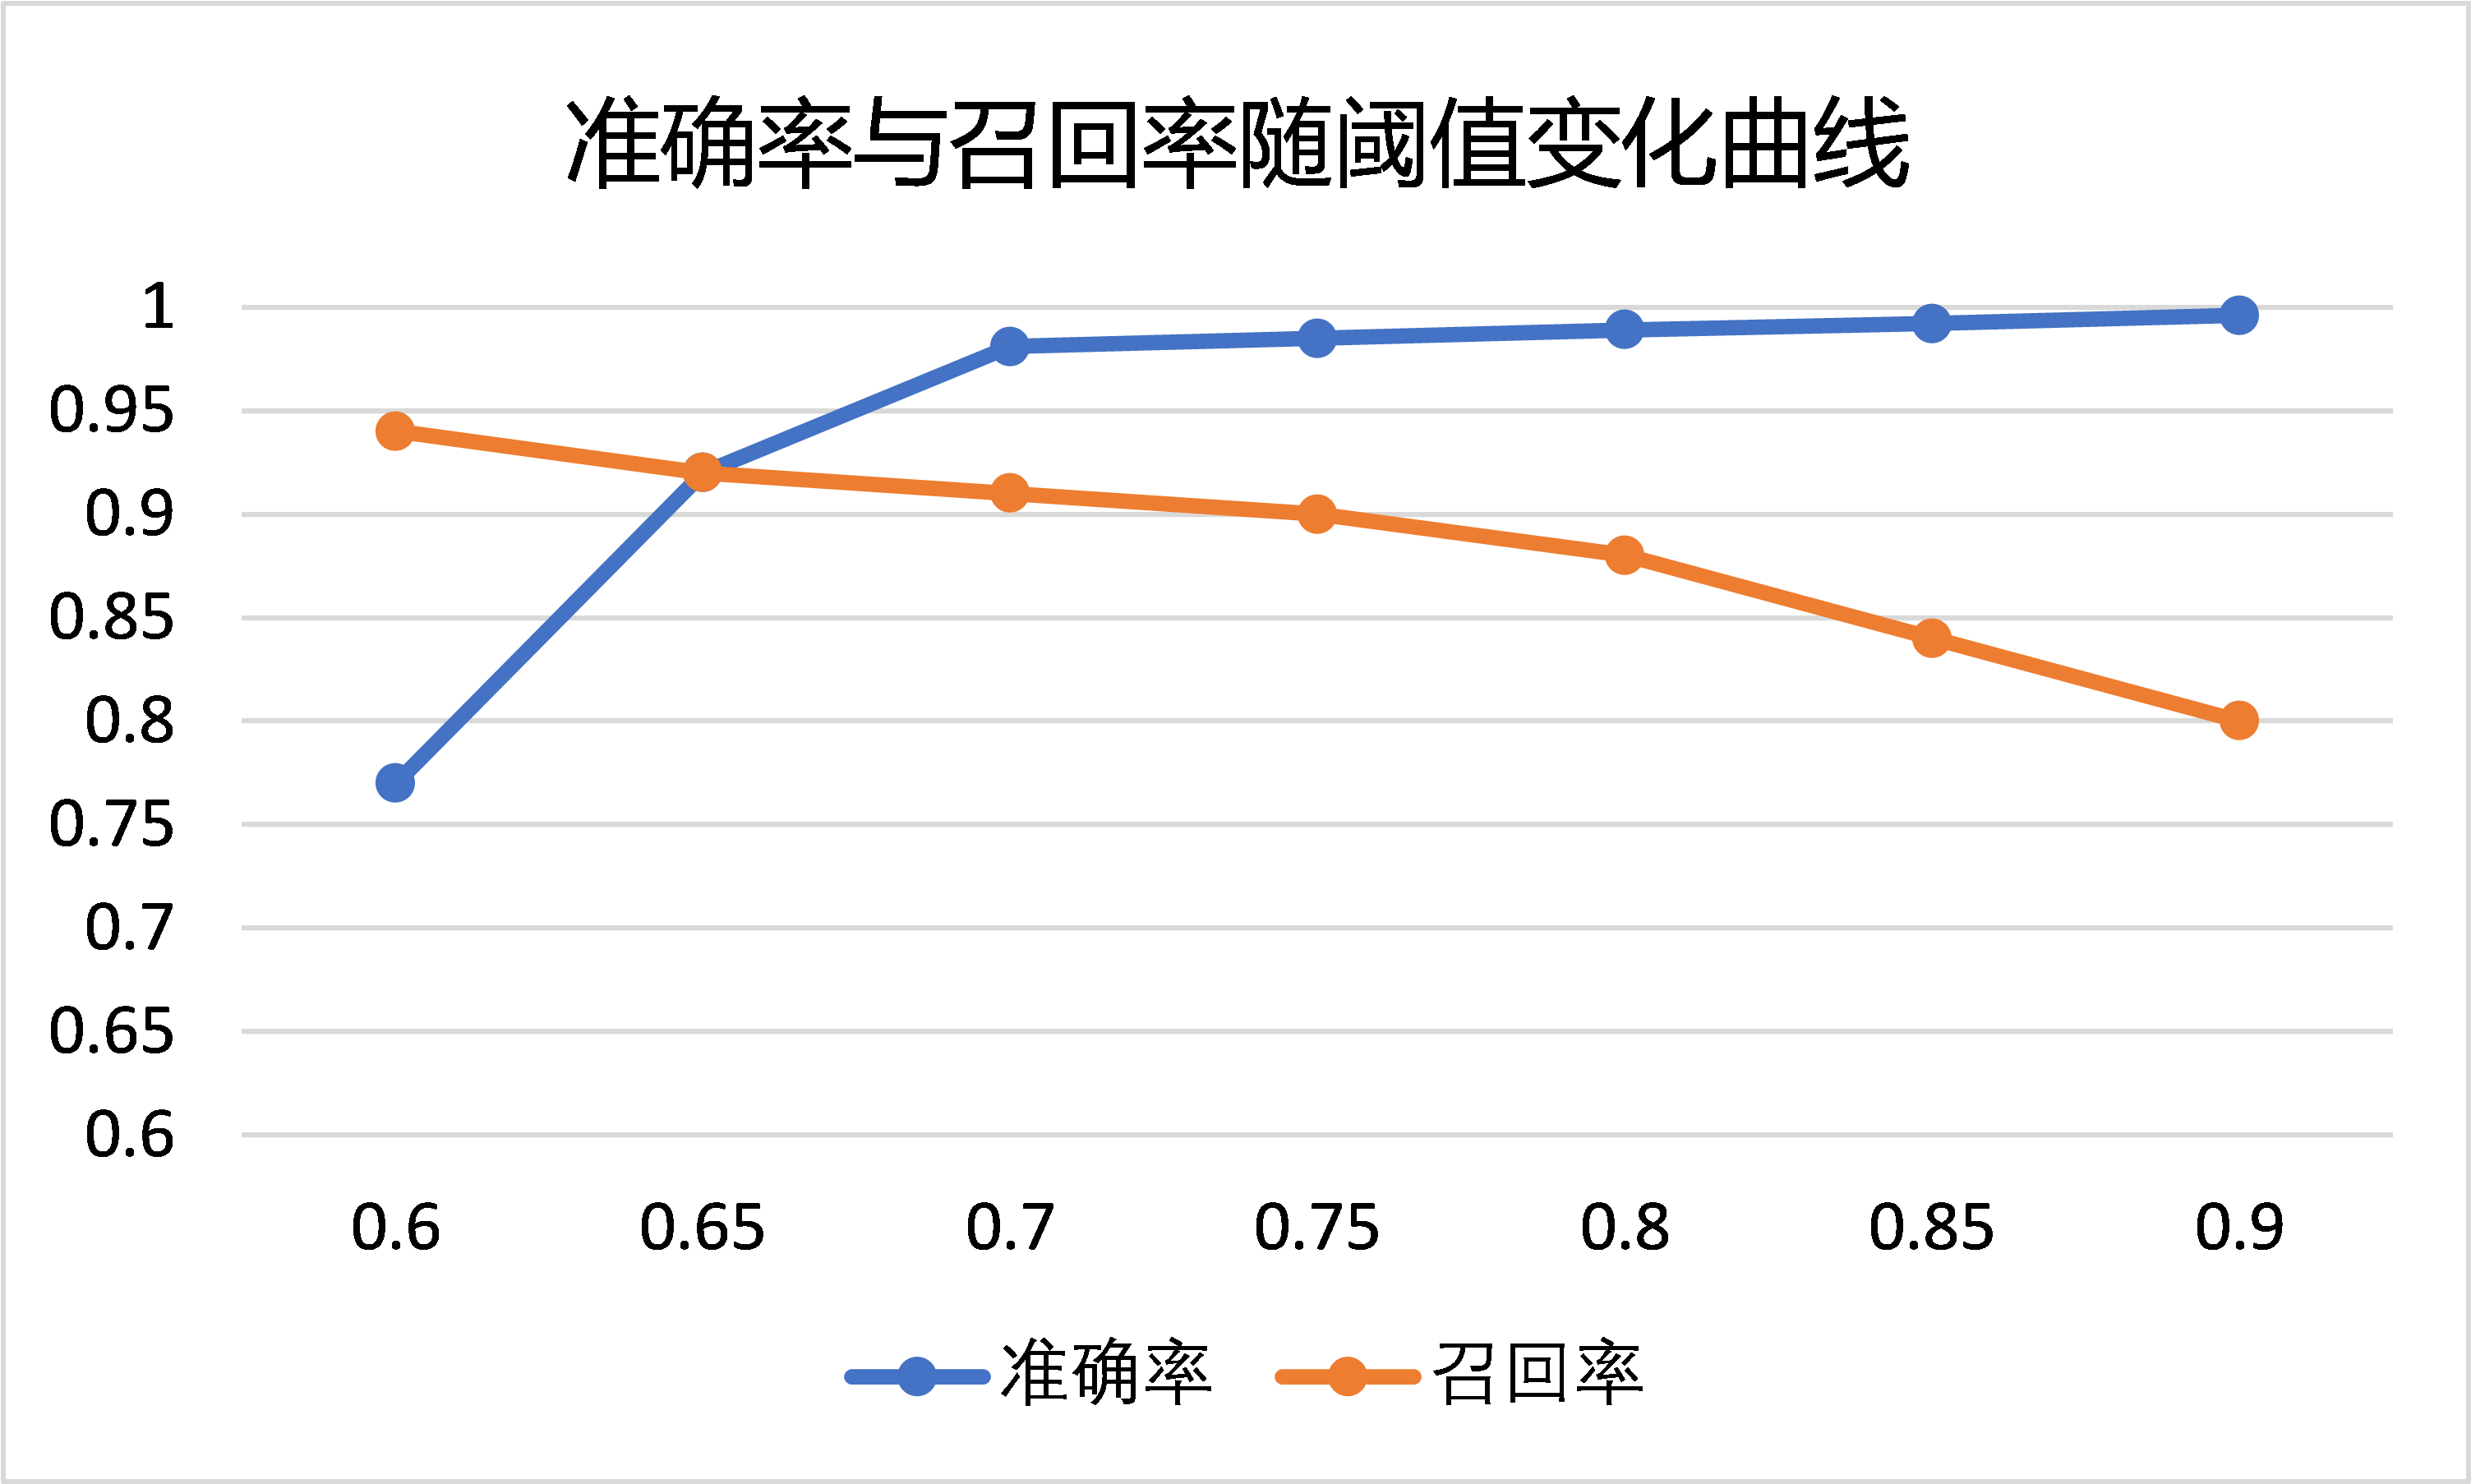
\includegraphics[width=12cm]{threshold.png} \\
  \caption{准确率与召回率随阈值变化曲线}
 \label{fig:threshold}
\end{figure}


阈值选定后,进行App与标准库的匹配。对每一个App中划分出的每一个包,先采用粗粒度特征匹配算法\ref{algo:coarse_exp}选出该包所对应的库,再采用细粒度特征匹配算法识别出库的具体版本。由于阈值的设定,每个App的包可能在标准库数据库中有多个匹配结果,实验将这些结果都加入到匹配列表中,表示这些库是在现有知识下得出的结论。为了能够有效计算准确度,定义有效样本数为列表长度的倒数,因此若列表中只包含一个库,即系统选出了唯一的最佳匹配结果,那么此样本在评估指标计算的真阳性(TP)样本数中占1,否则列表越长,表示此次匹配效果越差,即不确定性高,相应的真阳性样本数占据小于1的一个分数。各标准库详情见附录A。匹配结果如表\ref{tab:result}所示。

\begin{table}[!hpt]
  \caption{App对各标准库的包含情况}
  \label{tab:result}
  \centering
  \begin{tabular}{ccccccccccc} \toprule
%    \multicolumn{2}{c}{Item} \\ \cmidrule(r){1-2}
      \diagbox{Lib}{App}& 1 & 2 & 3 & 4 & 5 & 6 & 7 & 8 & 9 & 10 \\ \midrule
	Google Ads & \ding{51} & \ding{51} & \ding{51} & \ding{51} & \ding{51} & \ding{55} & \ding{51} & \ding{51} & \ding{51} & \ding{51}  \\
	Apache Http & \ding{51} & \ding{55} & \ding{51} & \ding{55} & \ding{55} & \ding{51} & \ding{51} & \ding{55} & \ding{55} & \ding{55} \\
	Firebase & \ding{51} & \ding{51} & \ding{51} & \ding{55} & \ding{55}* & \ding{55} & \ding{55} & \ding{55} & \ding{55} & \ding{55} \\
	Square Dagger & \ding{51} & \ding{55} & \ding{55} & \ding{51} & \ding{51} & \ding{55} & \ding{55} & \ding{55} & \ding{55} & \ding{55}\\
	ChartBoost & \ding{55} & \ding{55} & \ding{55} & \ding{51} & \ding{55} & \ding{55} & \ding{55} & \ding{51} & \ding{55} & \ding{55}\\
	JavaX Annotation & \ding{51} & \ding{55} & \ding{55} & \ding{55} & \ding{55} & \ding{55} & \ding{55} & \ding{55} & \ding{55} & \ding{55}\\
	OKHttp3.0 & \ding{51} & \ding{55} & \ding{55} & \ding{55} & \ding{55} & \ding{55} & \ding{55} & \ding{55} & \ding{55} & \ding{55}\\
	Tencent SDKs & \ding{55} & \ding{55} & \ding{55} & \ding{55}* & \ding{55} & \ding{55} & \ding{51}* & \ding{55} & \ding{55} & \ding{55}\\
	ksoap2 & \ding{55} & \ding{55} & \ding{55} & \ding{55} & \ding{55} & \ding{55} & \ding{55} & \ding{55} & \ding{55} & \ding{51}\\
	 \bottomrule
  \end{tabular}
    \begin{tablenotes}
    \item \quad \quad \quad \quad *表示检测结果错误。% or \item [a]
    \end{tablenotes}
\end{table}


系统各评估指标结果如表\ref{tab:metric}所示,TPL-V Detector在准确率上表现较好,误报率很低,但是没有将App中使用到的库全部召回。查看各库的版本情况发现,识别出错较多的库——腾讯SDK(tencentcloud-sdk-java-common)包含了276个版本,仅版本3.1.x的子版本号就超过了100个,本身各版本之间的差异可能不大,而混淆后的App中经过了代码优化、压缩等过程,导致部分未用到的代码被删去,有一定可能损失包含关键区别的部分特征,最后使得系统在此库上表现不佳。

\begin{table}[!hpt]
  \caption{TPL-V Detector各项指标评估结果}
  \label{tab:metric}
  \centering
  \begin{tabular}{cc} \toprule
%    \multicolumn{2}{c}{Item} \\ \cmidrule(r){1-2}
    指标 &  评估结果 \\ \midrule
	Accuracy & 98.5\% \\
	Precision & 88.0\% \\
	Recall & 81.5\% \\
	F1\_score & 84.6\% \\
	FPR & 0.6\% \\
	 \bottomrule
  \end{tabular}
\end{table}


\subsubsection{时间开销实验}

为了细致评估TPL-V Detector的时间开销,实验将从取得App到完成库匹配的整个流程分成了如图\ref{fig:flow}所示的四个部分,分别为:
\begin{enumerate}
\item {App预处理}
\item {字节码特征提取}
\item {特征树构建}
\item {特征存储与匹配}
\end{enumerate}
其中App预处理又包含了Apk的解压、Dex文件的反编译、Class文件到Bytecode文件的转换,以及小于1KB文件的过滤。字节码特征提取包含了基于方法描述符的粗粒度特征的提取和基于字节码指令序列的细粒度特征的提取。特征树的构建自下而上从方法层到类层构建特征。特征的存储与匹配分为特征向MySQL的存储,以及特征的粗粒度/细粒度两级特征匹配。


\begin{figure}[!htp]
  \centering
  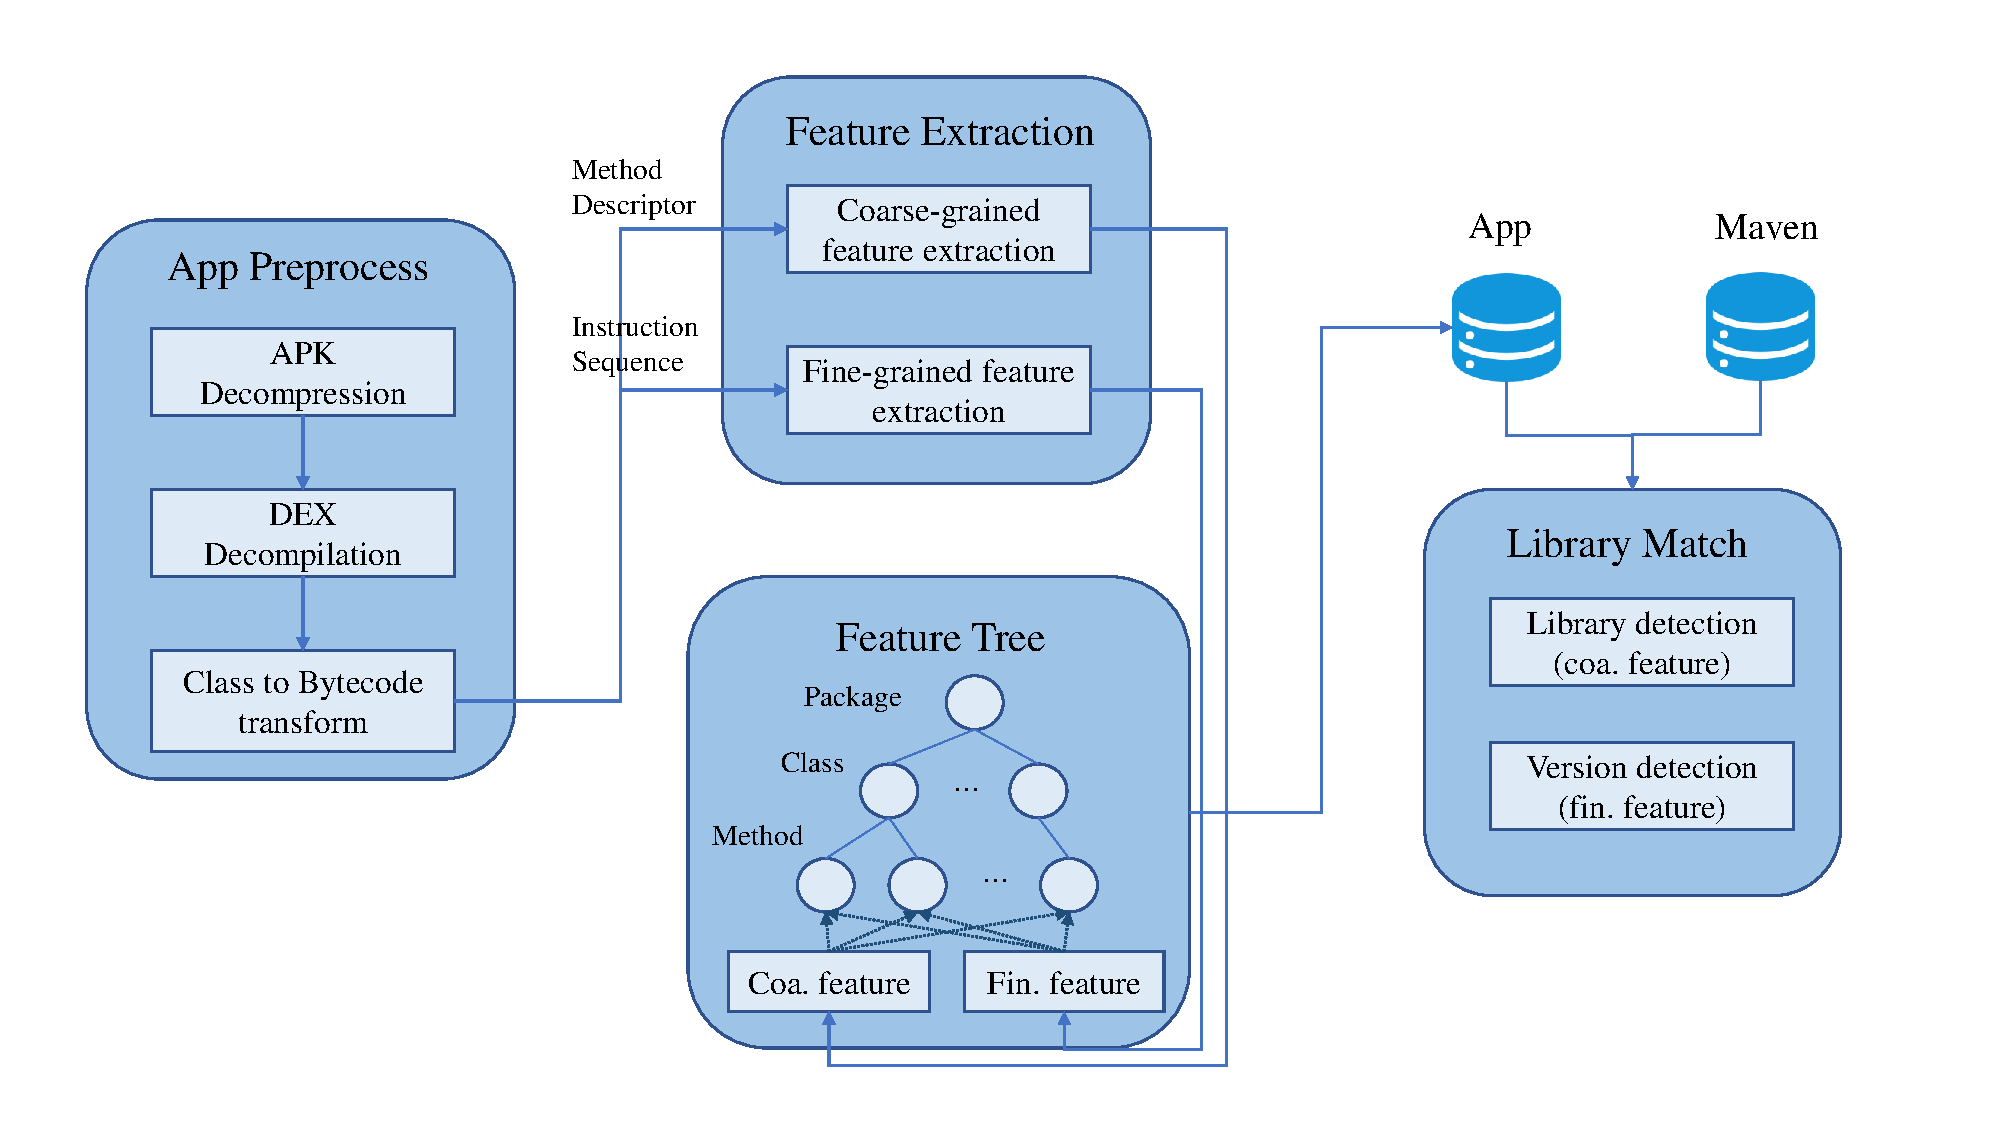
\includegraphics[width=15cm]{flow.pdf} \\
  \caption{时间开销测试App库匹配的四阶段工作流程}
 \label{fig:flow}
\end{figure}

对于实验所用十款App,按照文件大小排序,分别测试其各阶段所用时间,测试结果如图\ref{fig:flow}所示。对于一个大小为15MB的App,执行完四个阶段所需耗时仅仅约半分钟。最大的App大小为258MB,处理时间开销已经接近了十分钟。在四个阶段中,阶段一耗时占比最大,基本都超过了总耗时的一半。经过对阶段一进一步分析,我认为可能是调用第三方工具所导致。对App的预处理首先需要调用unzip解压工具,获取DEX文件;对DEX文件,需要借助github开源工具dex2jar来获取class文件;最后class文件转换成字节码的过程中需要频繁的使用javap程序,累积产生了较大的时间开销。阶段二特征提取耗时较少,主要原因可能是此阶段只需要进行文本读取操作,并且为了过滤掉不包含方法的类,TPL-V Detector还会删除小于1KB的字节码文件,进一步节省了时间。阶段三是耗时最少的步骤,此部分由C++代码实现,数据结构较为繁杂,但是处理流程高效,将原始的粗细特征处理成方法的粗细特征,并将包/类/方法组织成树形结构,生成类的特征即可。第四阶段耗时占比在15\%至30\%之间,此部分耗时实际上依赖于先验知识数据库的大小,数据库越大,则匹配耗时越长;数据库小,则匹配的时间开销就很少。




\begin{figure}[!htp]
  \centering
  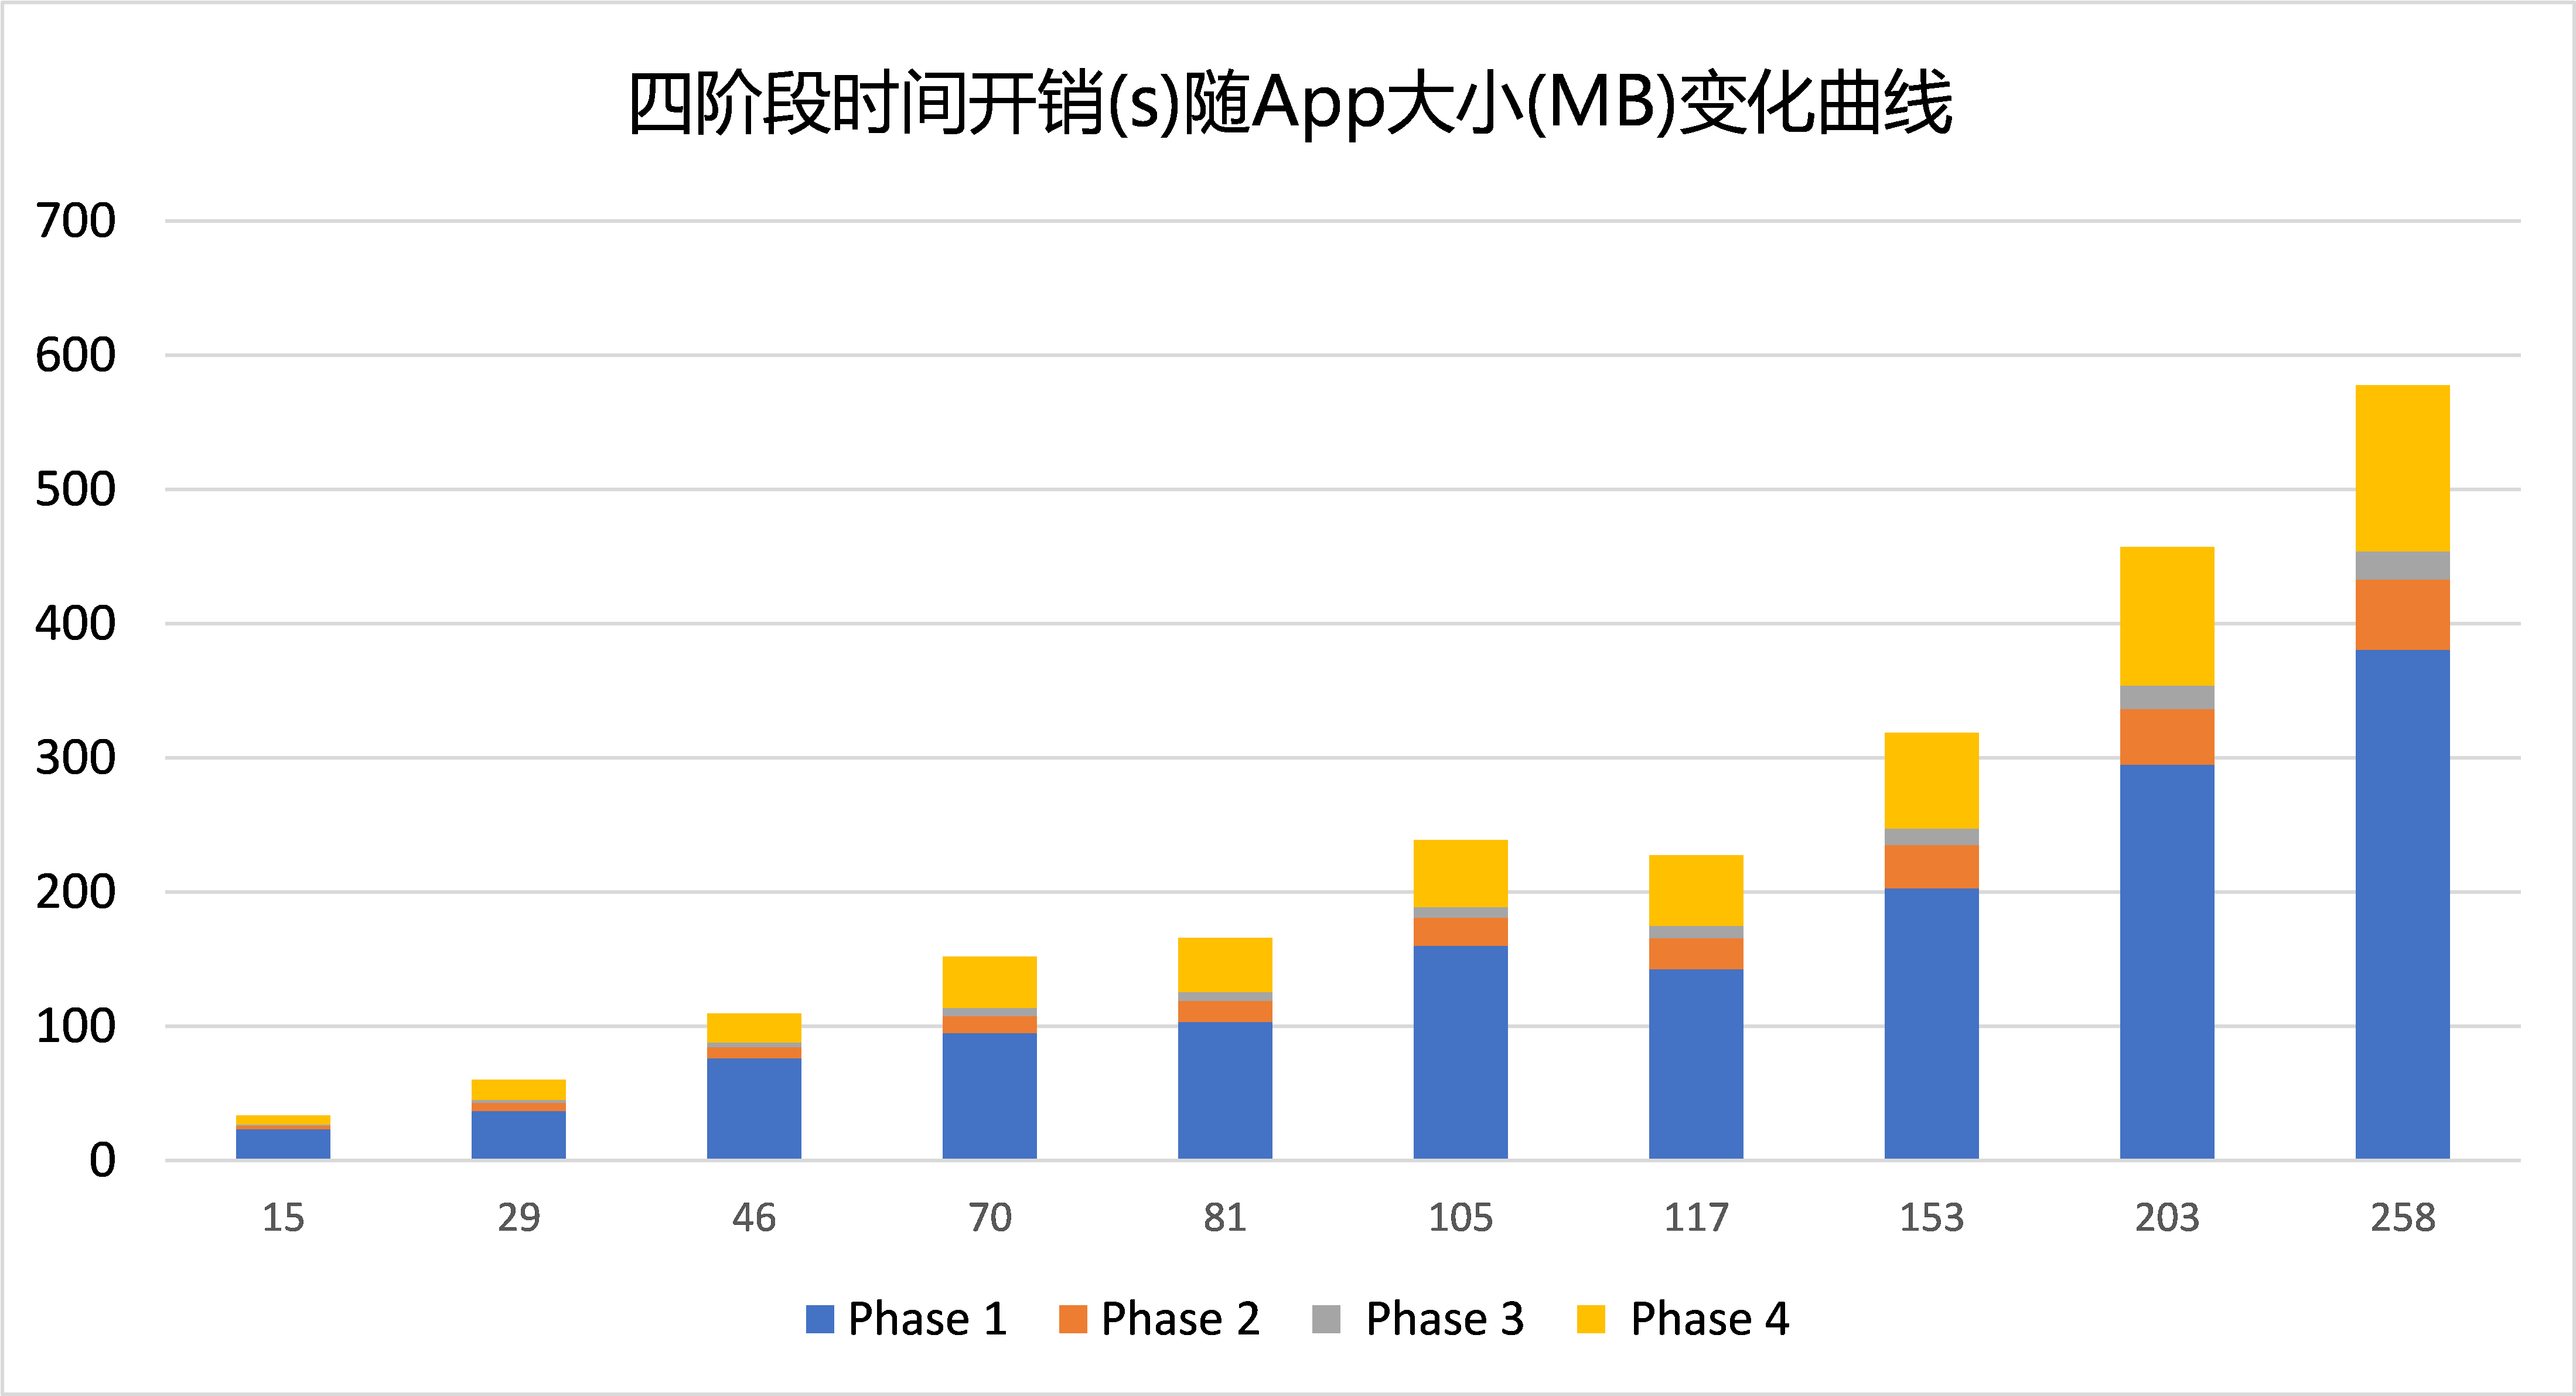
\includegraphics[width=11cm]{time.png} \\
  \caption{各阶段时间开销随App大小变化曲线}
 \label{fig:flow}
\end{figure}


Apk文件越大,包含的DEX文件就大,相应的class文件、字节码文件、产生的特征就更多,作为根包生成特征树的目录也更多,匹配耗时越长。反之亦然,App规模小,各阶段耗时也有所下降。根据图\ref{fig:four},四个阶段的时间开销与App大小基本上呈现出线性关系。

\begin{figure}[!htp]
  \centering
  \begin{subfigure}{0.4\textwidth}
    \centering
    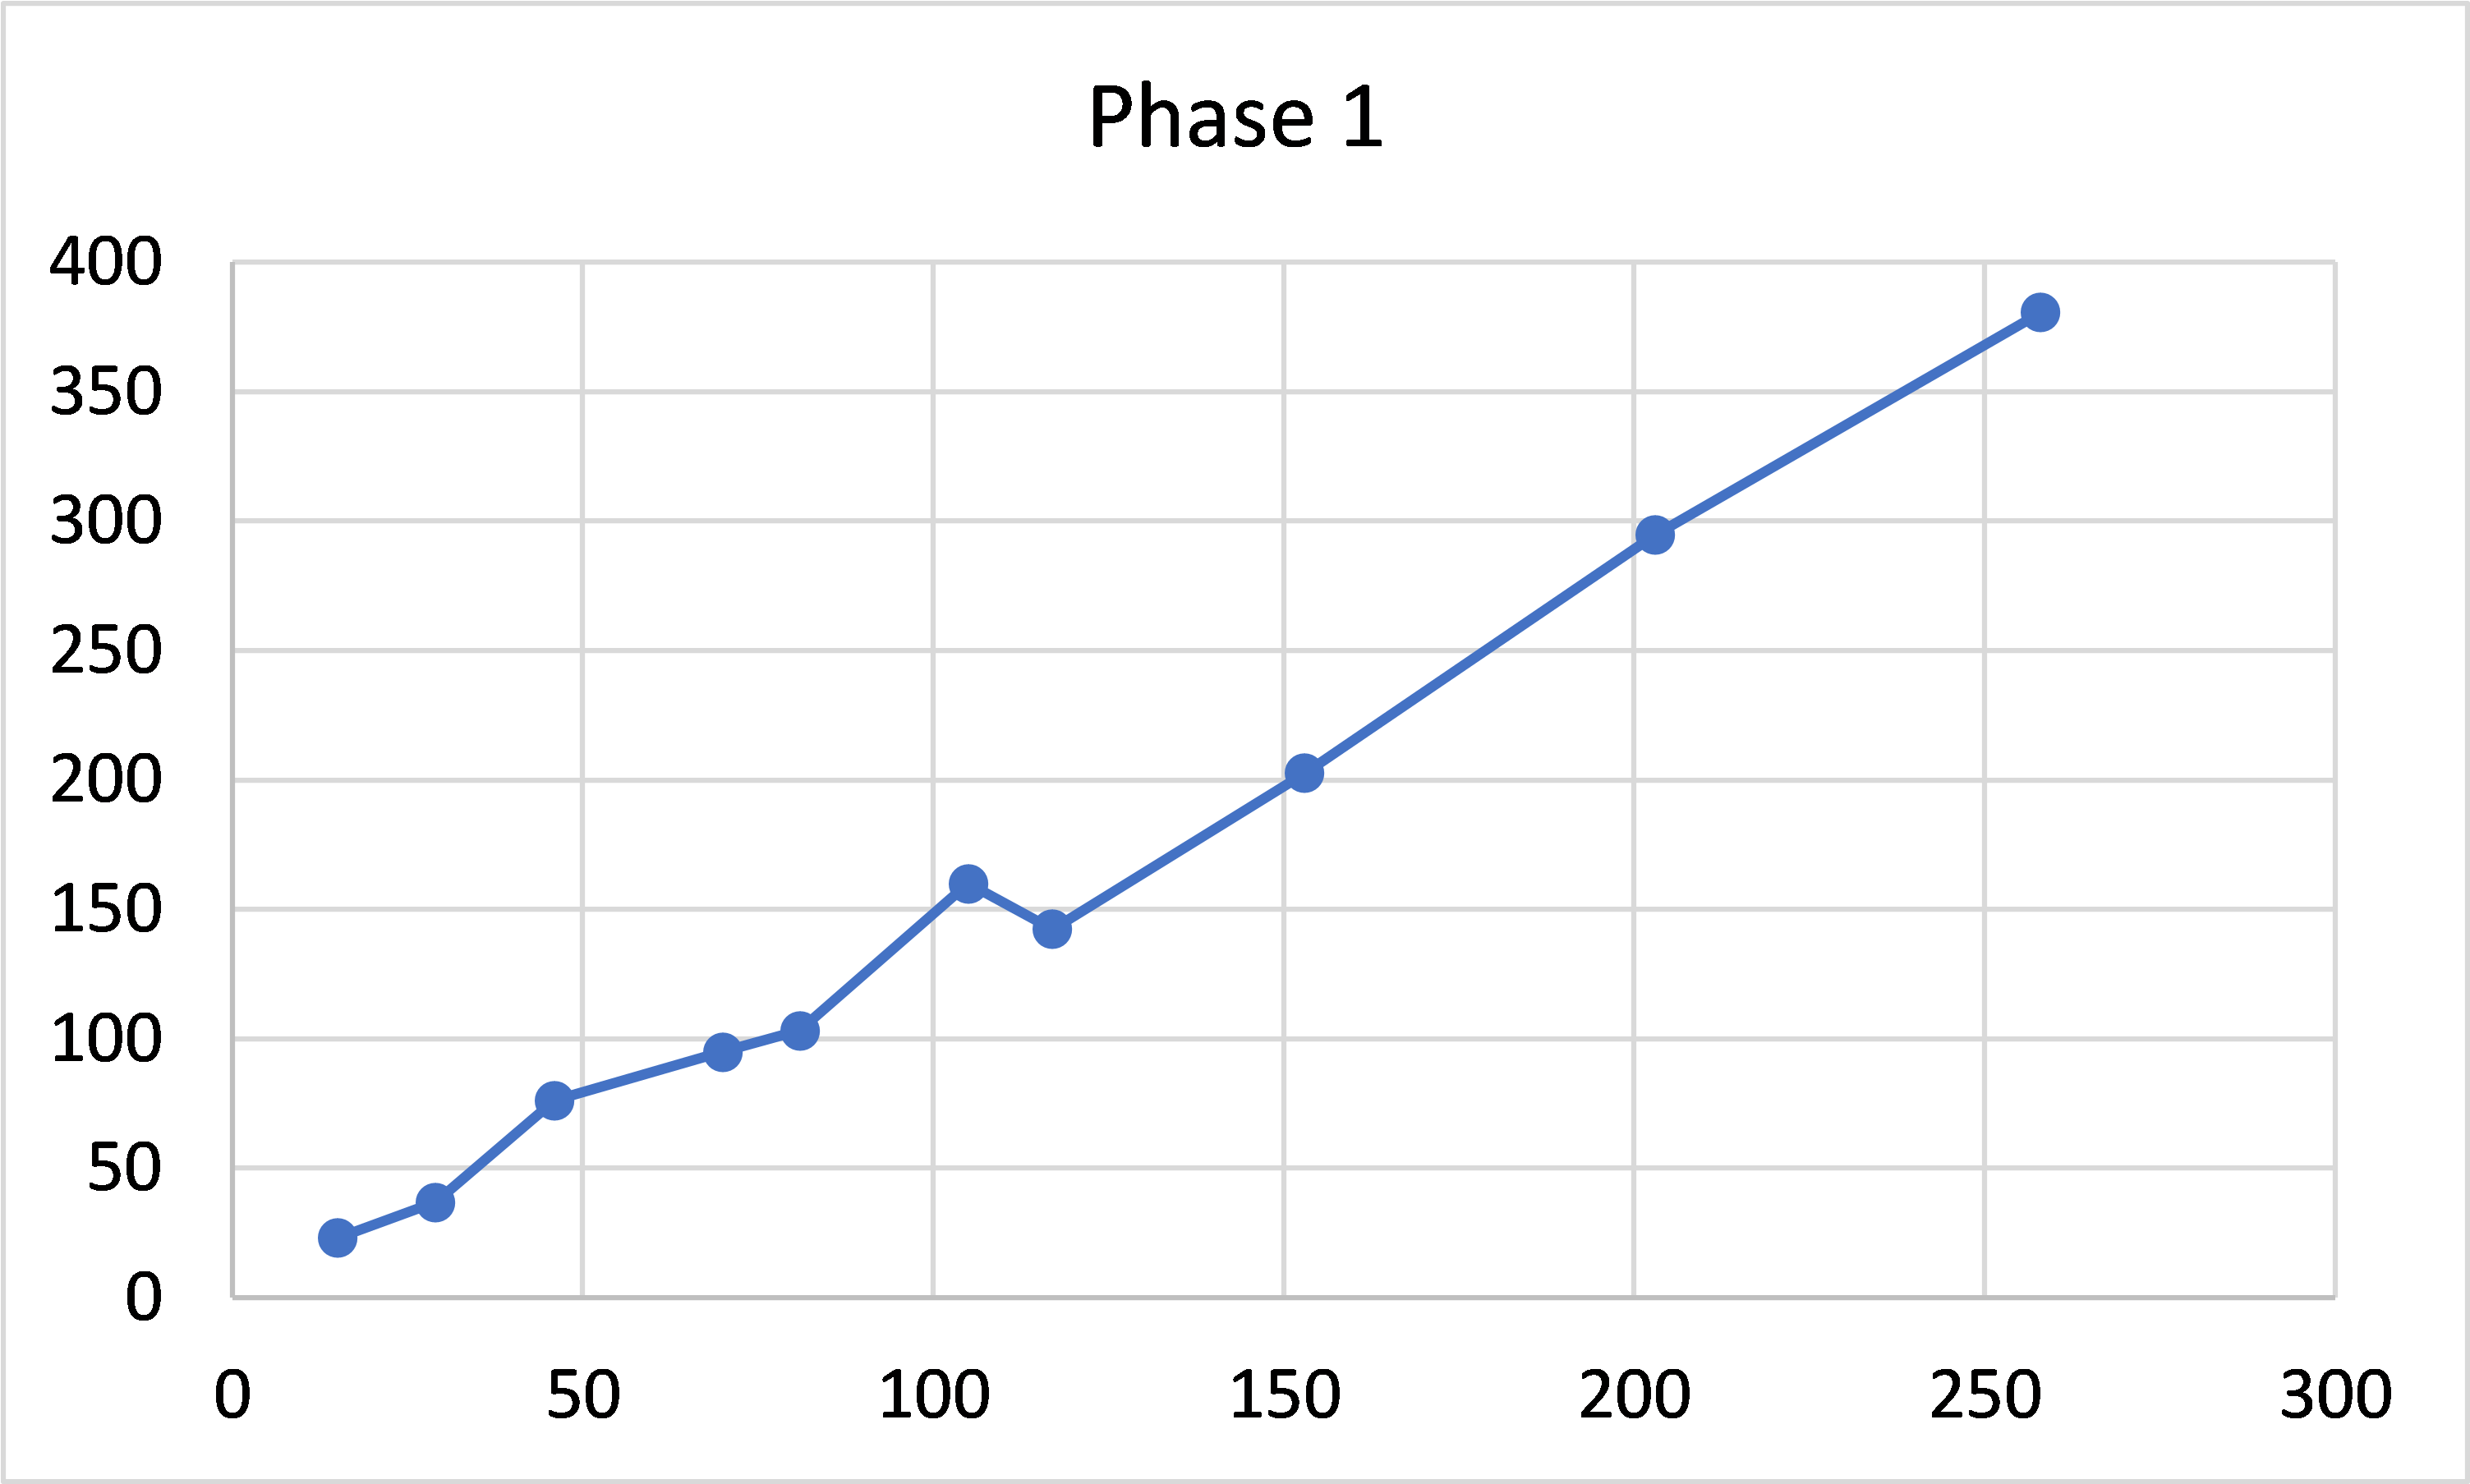
\includegraphics[height=4cm]{f1.png}
    \caption{App预处理阶段时间开销}
  \end{subfigure}
  \hspace{1cm}
  \begin{subfigure}{0.4\textwidth}
    \centering
    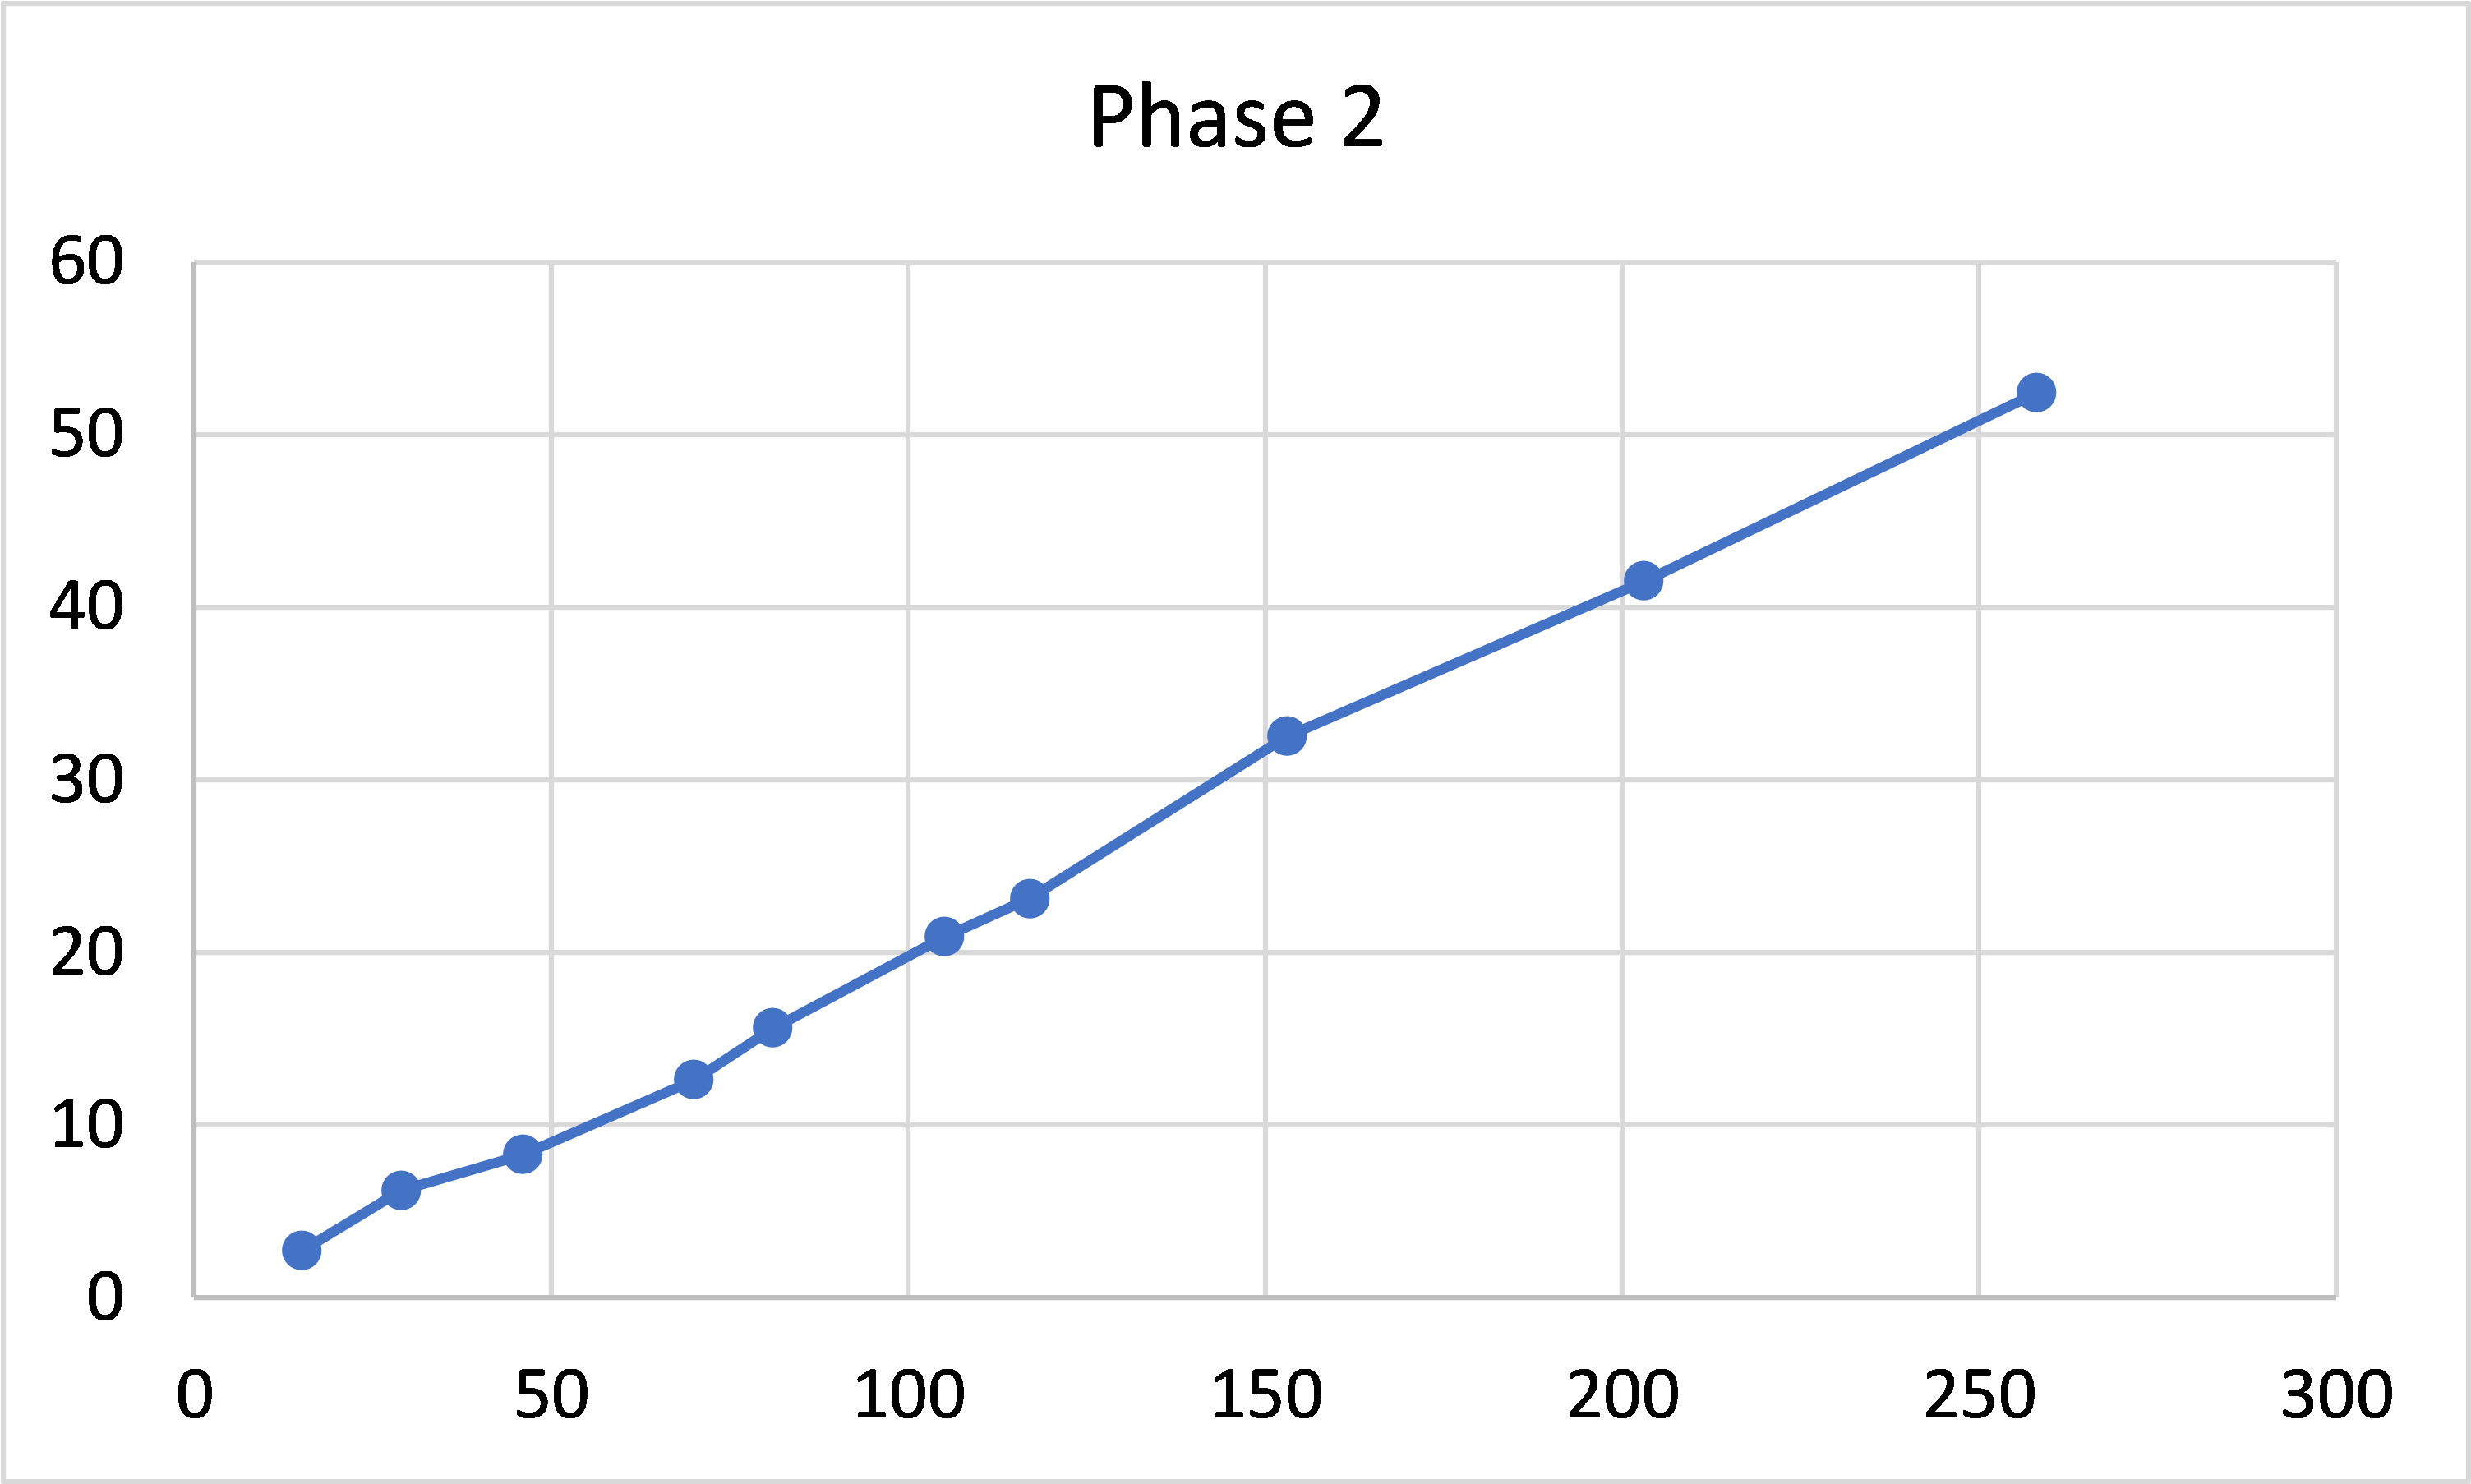
\includegraphics[height=4cm]{f2.png}
    \caption{特征提取阶段时间开销}
  \end{subfigure}
  \vfill
  \begin{subfigure}{0.4\textwidth}
    \centering
    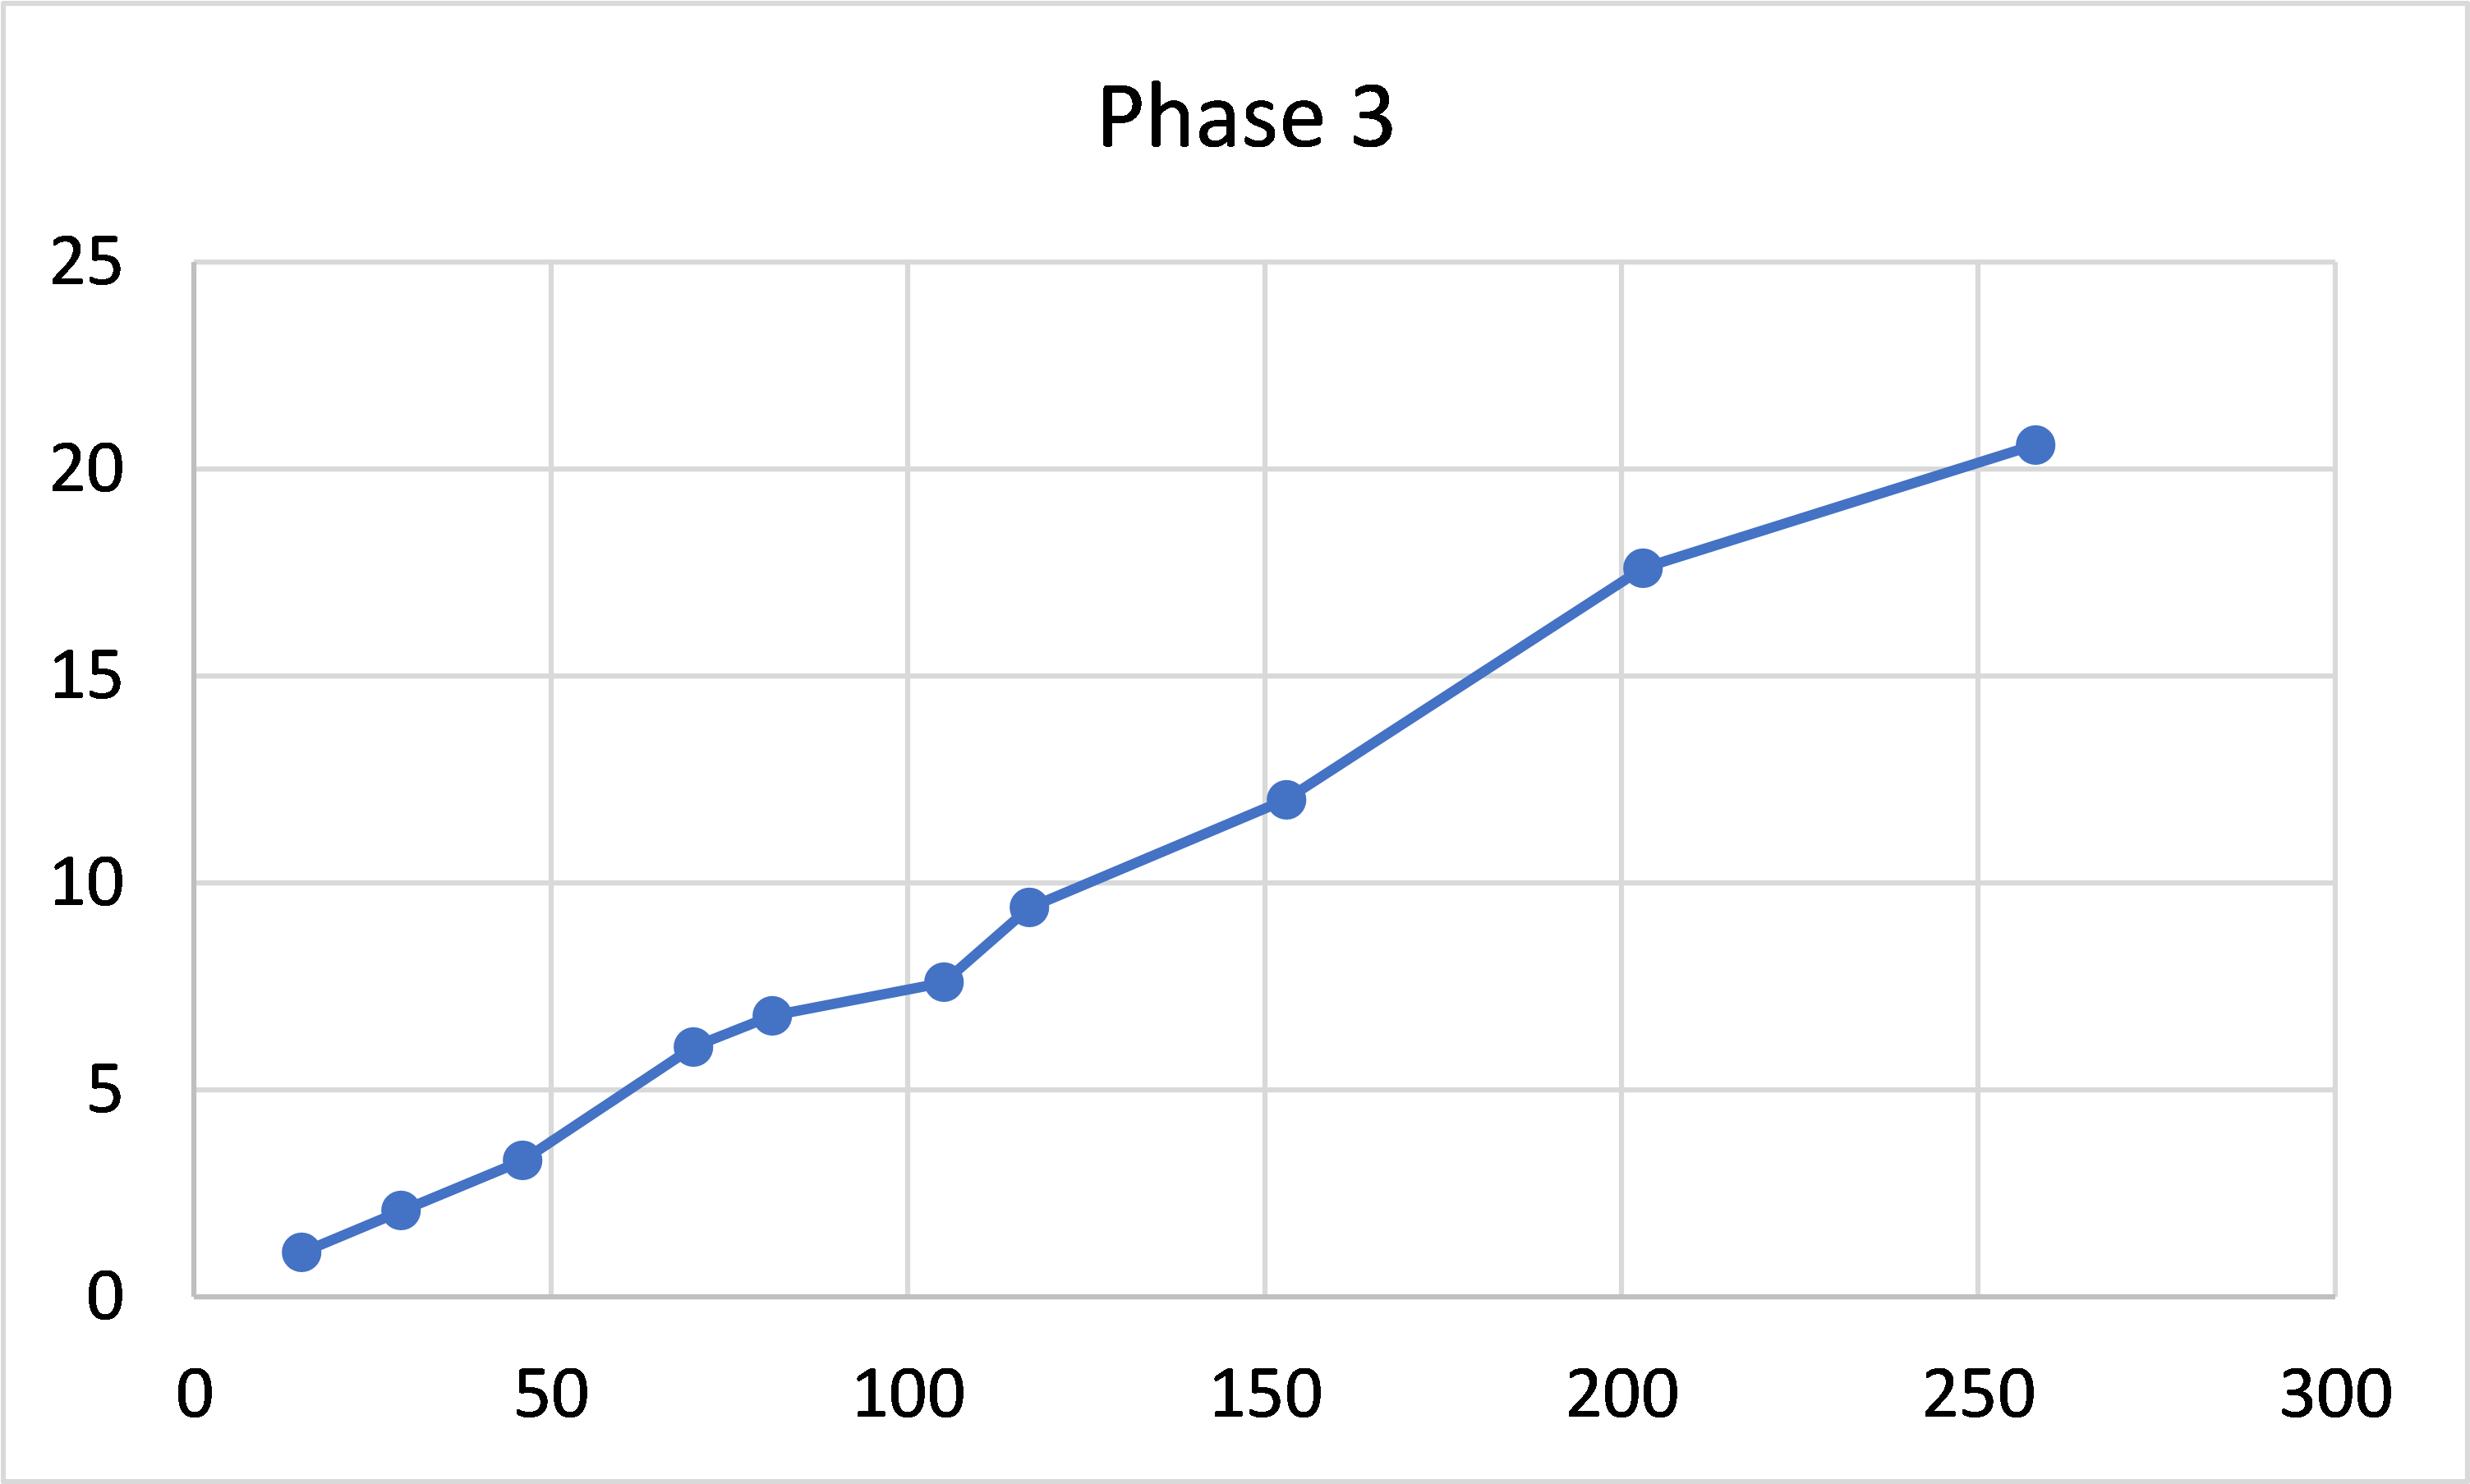
\includegraphics[height=4cm]{f3.png}
    \caption{特征树构建阶段时间开销}
  \end{subfigure}
  \hspace{1cm}
  \begin{subfigure}{0.4\textwidth}
    \centering
    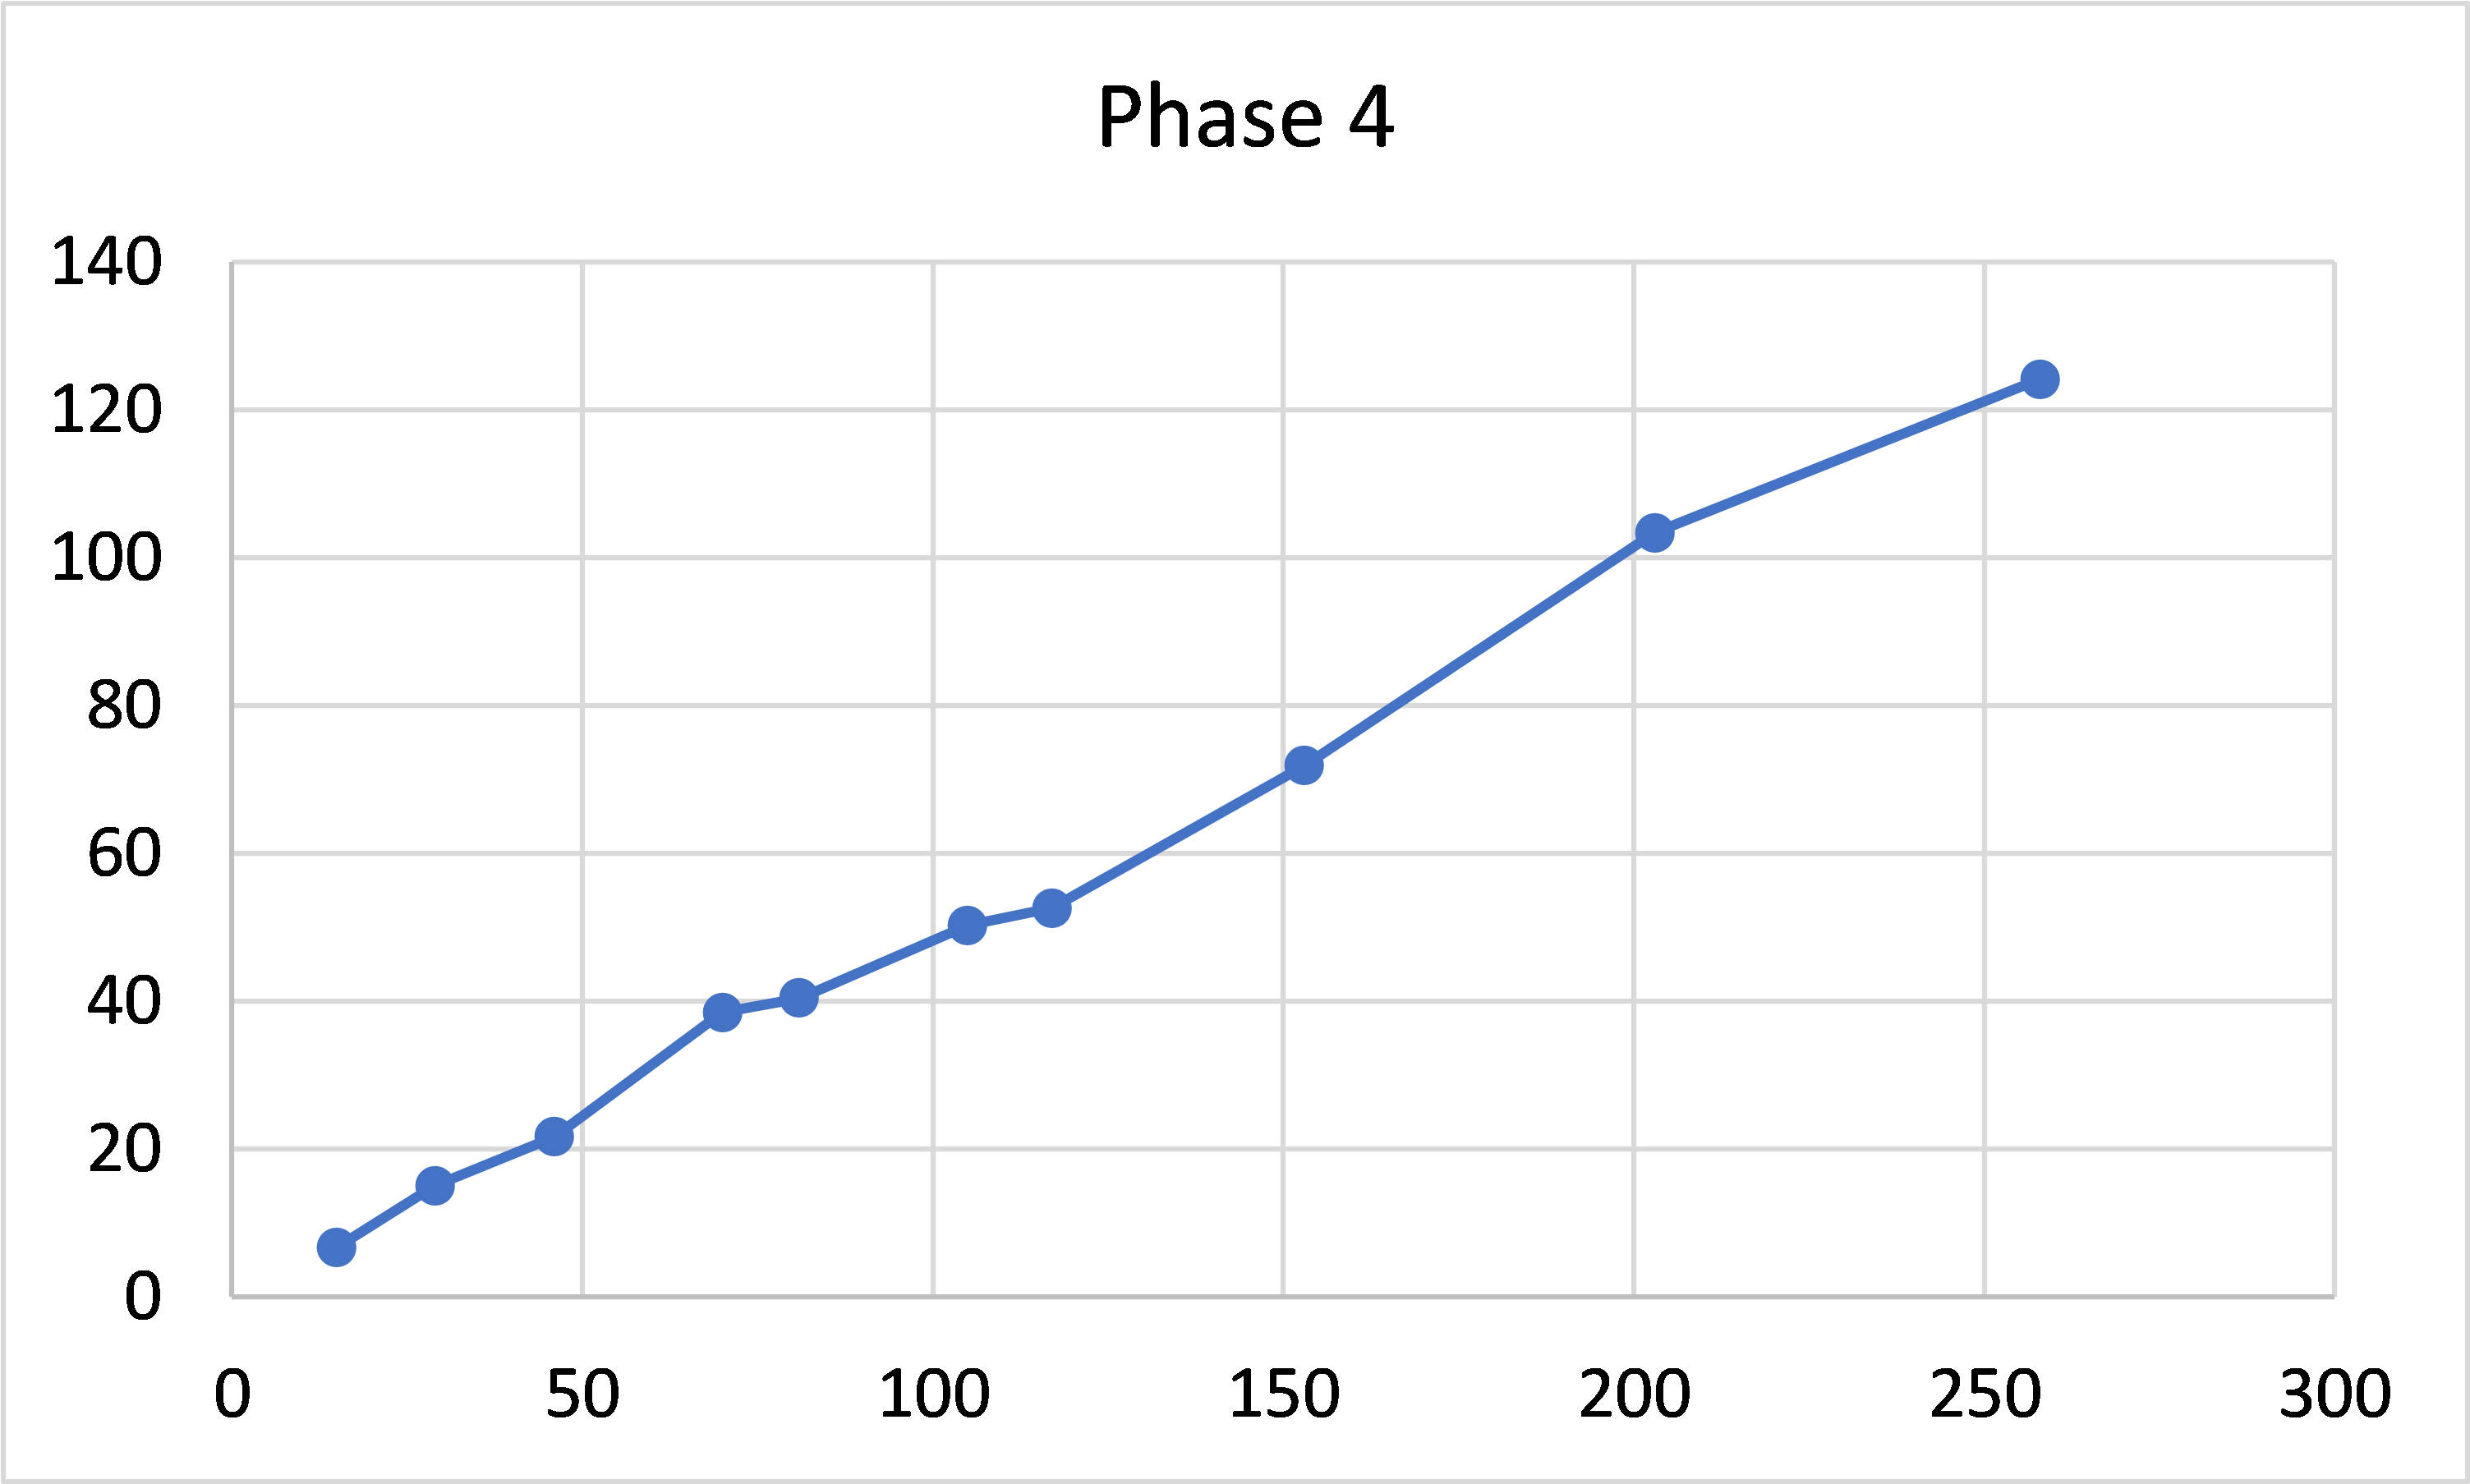
\includegraphics[height=4cm]{f4.png}
    \caption{特征存储与匹配阶段时间开销}
  \end{subfigure}
  \caption{各阶段时间开销(s)随App大小(MB)变化曲线}
  \label{fig:four}
\end{figure}


\subsection{匹配策略的加速效果实验}

两级特征与优先级队列的匹配策略可以提高TPL-V Detector的匹配速度。为检验其加速效果,本文选择了来源于Mumayi\cite{mumayi}的一款App,针对其所包含的okio、okhttp两个库进行匹配实验。图\ref{fig:acc}展示了匹配阶段在仅使用细粒度特征匹配、使用两级特征匹配、使用细粒度特征与优先级队列、使用两级特征与优先级队列四种情况下的时间开销随数据库大小的变化情况。

\begin{figure}[!htp]
  \centering
  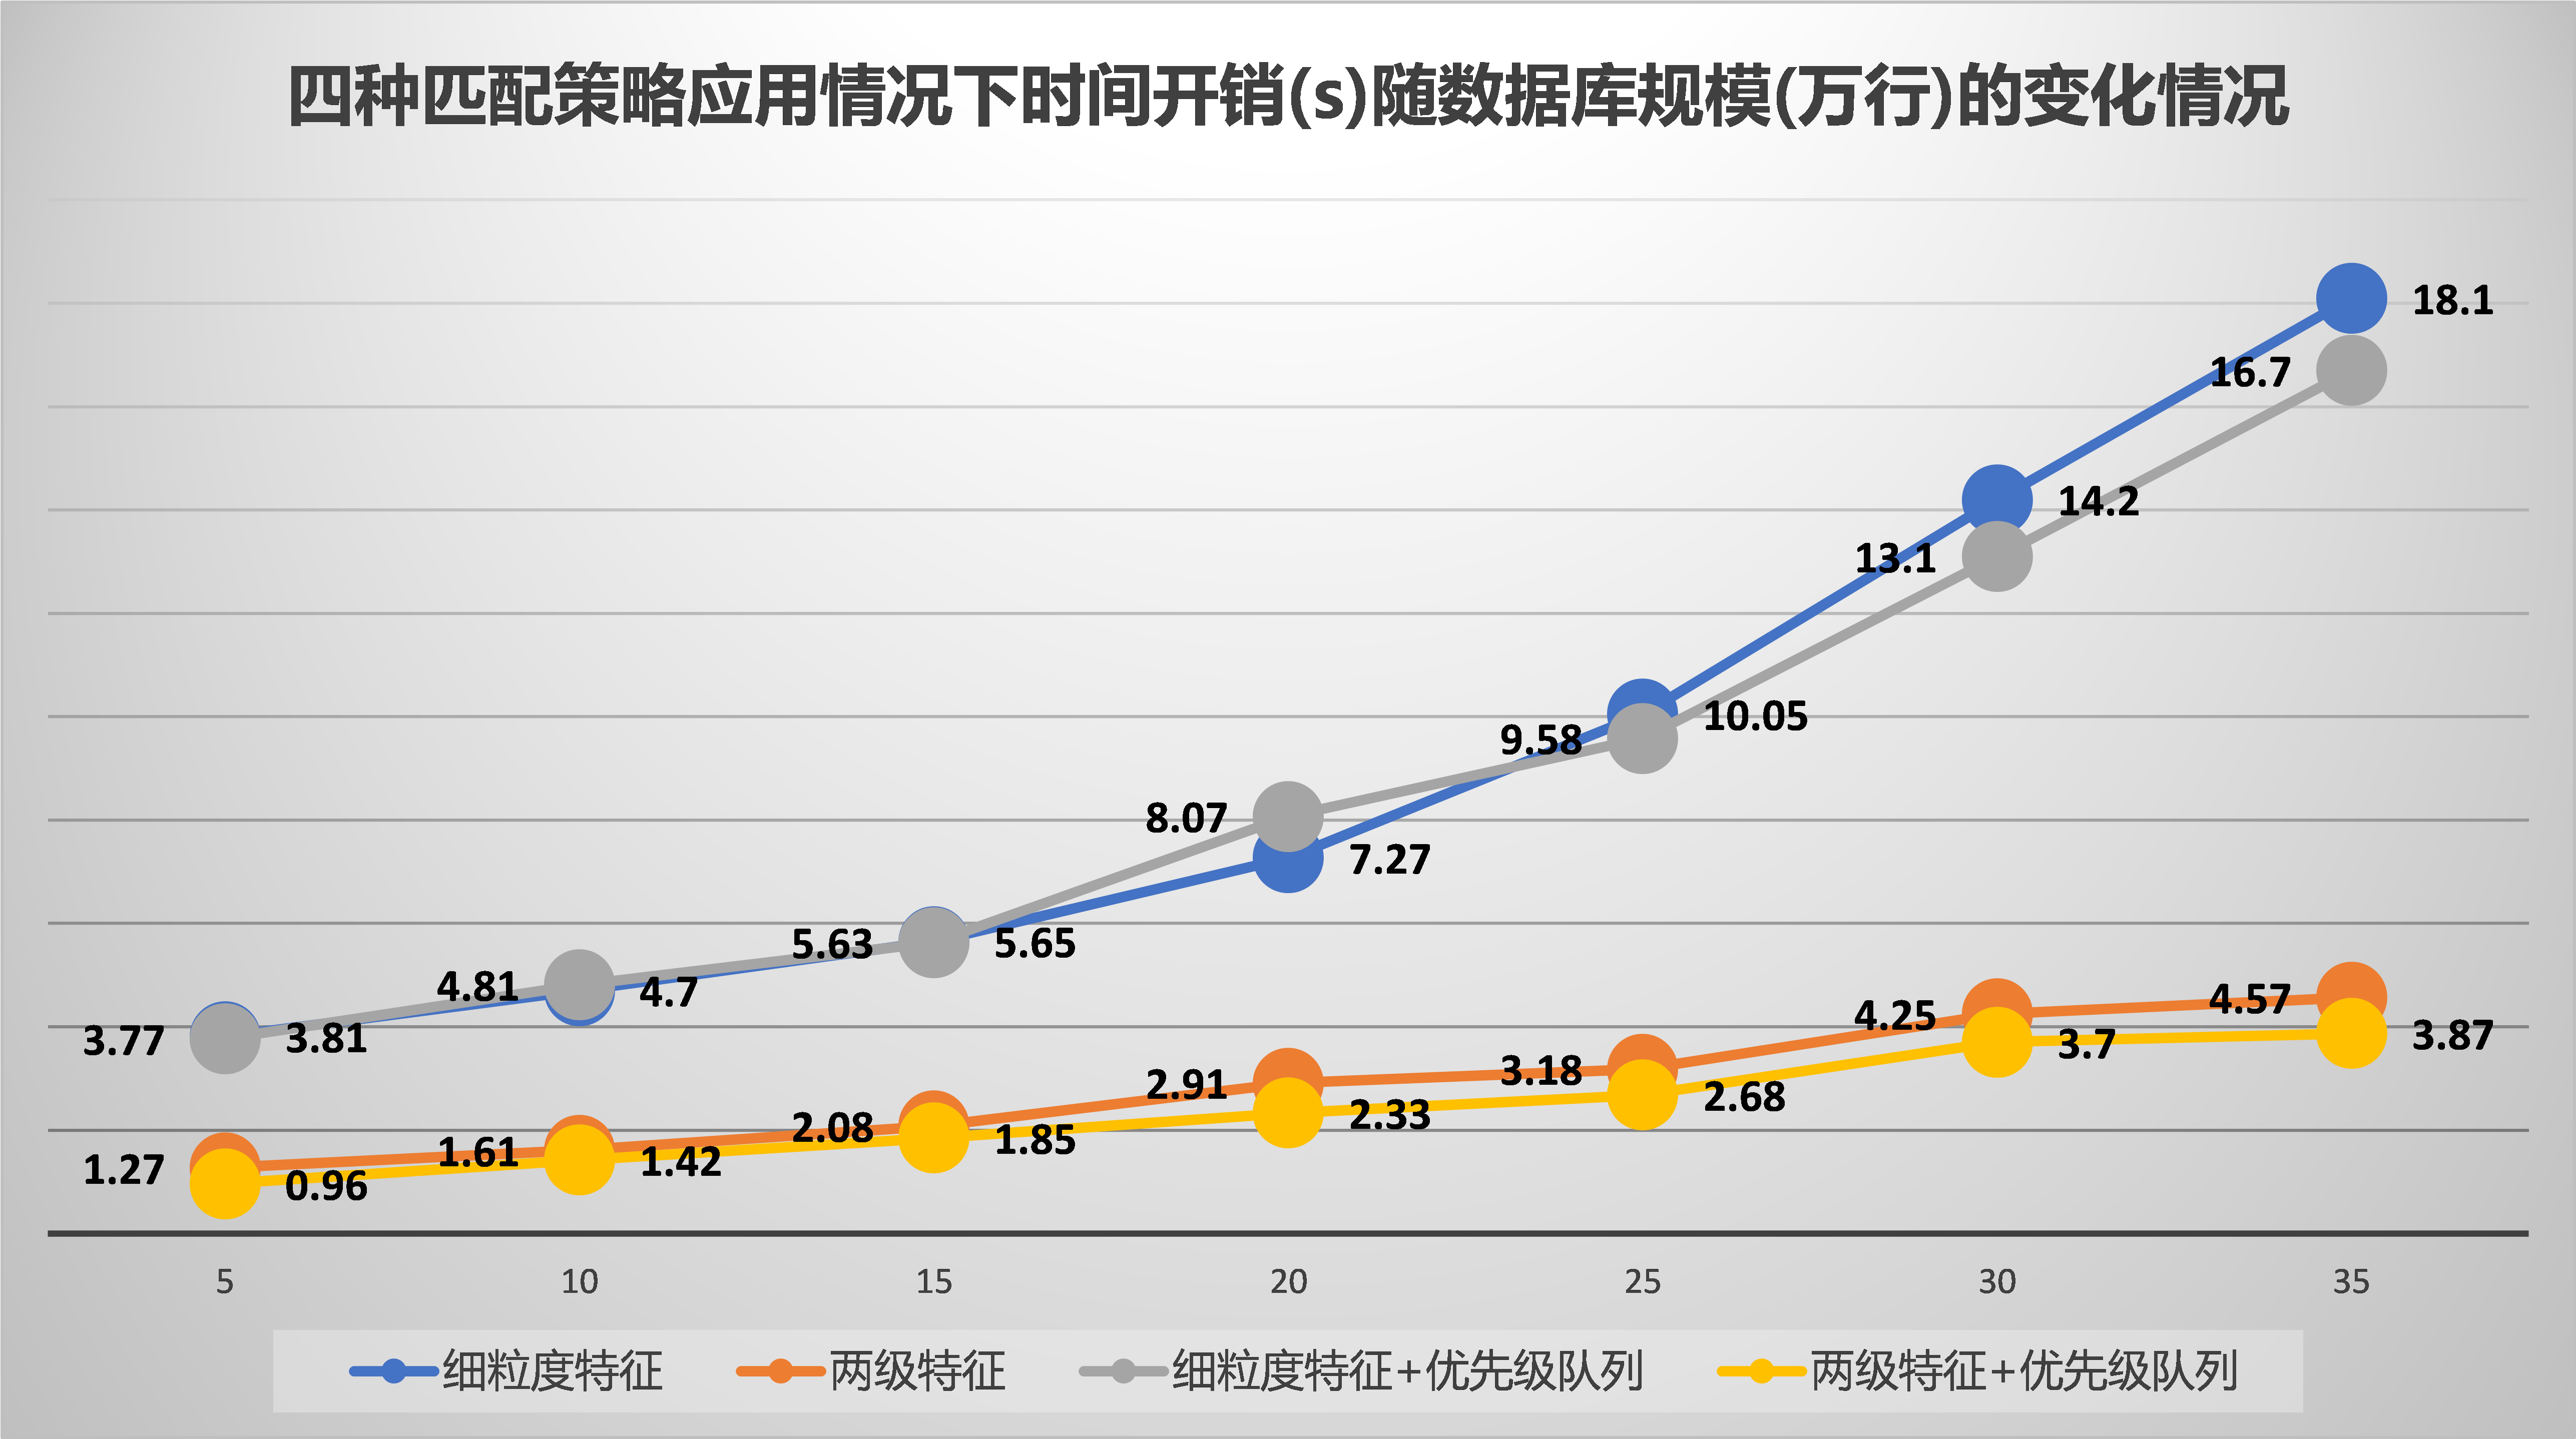
\includegraphics[width=11cm]{acc.png} \\
  \caption{四种匹配策略应用情况下时间开销(s)随数据库规模(万行)的变化情况}
 \label{fig:acc}
\end{figure}

从图中可以看出,两级特征策略对时间开销的影响较为显著,这是因为细粒度计算方法复杂,特征序列较长,而粗粒度特征计算简单快捷,首先使用粗粒度特征限制范围,对于不合格的匹配对之间略过,可以有效减少大量不必要细粒度特征的匹配次数。相比之下,优先级队列策略对时间开销的优化功能不太稳定,在应用两级特征的前提下对匹配速度有所提升,但在仅使用细粒度特征时甚至会带来更大的时间开销。导致这种情况的一个可能原因是,影响时间的主要因素是特征的选择,当特征的计算与匹配工作过于繁杂时,是否应用优先级队列的影响相较而言小了很多,甚至当数据库规模增大时,优先级队列的创建、入队/出队等操作还会使得耗时不降反增。尽管如此,两级特征加优先级队列的策略仍然具有最好的时间表现。


\subsection{与现有工具的对比实验}

为评估TPL-V Detector的优越性与局限性,本文针对9个标准库,与现有的部分工具进行了对比实验,包括LibID\cite{zhang2019libid}、LibScout\cite{backes2016reliable}、Orlis\cite{wang2018orlis}和LibRoad\cite{xu2020libroad}。

\begin{table}[!hpt]
  \caption{各工具对分别对9个混淆标准库及其具体版本识别情况}
  \label{tab:compare}
  \centering
  \begin{tabular}{ccccc} \toprule
%    \multicolumn{2}{c}{Item} \\ \cmidrule(r){1-2}
     \diagbox{library}{tool} & TPL-V Detector & LibID & LibScout & Orlis  \\ \midrule
	Google Ads & \ding{51} & \ding{55} & \ding{51} & \ding{55} \\
	Apache Http & \ding{51} & \ding{55} & \ding{51} & \ding{55}\\
	Firebase & \ding{51} & \ding{55} & \ding{55} & \ding{55} \\
	Square Dagger & \ding{51} & \ding{51} & \ding{51} & \ding{51} \\
	ChartBoost & \ding{51} & \ding{51} & \ding{51} & \ding{51} \\
	JavaX Annotation & \ding{51} & \ding{51} & \ding{51} & \ding{51} \\
	OkHttp3.0 & \ding{51} & \ding{51} & \ding{51} & \ding{55} \\
	Tencent SDKs & \ding{51} & \ding{55} & \ding{55} & \ding{55} \\
	ksoap2 & \ding{51} & \ding{51} & \ding{51} & \ding{51} \\
	 \bottomrule
  \end{tabular}
\end{table}

表\ref{tab:compare}显示了各工具对标准库特定版本的识别情况。四款工具都提供了抵抗混淆的第三方库检测机制,能够检测出大部分混淆库,但是LibID和Orlis不提供区分具体版本的功能,在具有较多版本号的库上表现不佳,如超过270个版本号的Tencent SDKs。根据表\ref{tab:compmetric},TPL-V Detector综合精确率、召回率和F1得分表现最佳。导致精确率降低的原因可能是阳性样本经过混淆,某些包含方法数较多的类没有被使用到而被删除,又由于其在计算库相似度得分时占据了较大的比重,因此最后得分无法超过阈值,因而被排除在结果外。导致召回率降低的原因可能是部分第三方库包含版本数目巨大,各版本之间差异小。在匹配过程中由于相似度超过了阈值而大量进入结果列表,按照样本计数方法,真正的结果所占样本数仅为结果列表长度$n$的倒数$1/n$,假阳性样本数为$1-1/n$,使得召回率减小。


\begin{table}[!hpt]
  \caption{TPL-V Detector各项指标评估结果}
  \label{tab:compmetric}
  \centering
  \begin{tabular}{cccc} \toprule
%    \multicolumn{2}{c}{Item} \\ \cmidrule(r){1-2}
    \diagbox{tool}{metric} & Precision & Recall & F1\_score  \\ \midrule
	TPL-V Detector & 88.0\% & 81.5\% & 84.6\% \\
	LibID\cite{zhang2019libid} & 68.7\% & 66.4\% & 67.5\% \\
	LibScout\cite{backes2016reliable} & 88.8\% & 42.3\% & 57.3\% \\
	Orlis\cite{wang2018orlis} & 60.4\% & 57.7\% & 59.0\% \\
	LibRoad\cite{xu2020libroad} & 67.8\% & 99.8\% & 77.1\% \\
	 \bottomrule
  \end{tabular}
\end{table}

\section{本章小结}
本章完成了TPL-V Detector检测性能与效率评估实验,展示了TPl-V Detector识别第三方混淆库的能力。4.1节首先介绍了TPL-V Detector的具体实现,设计了混淆库识别和实际App第三方库检测的实验流程,并设置了准确率、召回率等评价指标。4.2节声明了所使用的Maven数据集,对关键参数阈值$T_c$设置不同值进行了实验,选择表现最佳的值,最后针对所选6个库进行了混淆前后的匹配实验与性能评估,除了少数包含版本数较多的第三方库以外,TPL-V Detector均实现了准确的版本识别。4.3节进行了混淆App第三方库的检测实验,声明了所使用的安卓App数据集,并展示了TPL-V Detector对各第三方库的识别结果以及准确率、召回率等指标得分情况,进一步分析了系统各阶段的时间开销,提出了分析与思考,最后与现有论文LibID、LibScout等提出的检测方法进行了对比,在综合各指标考虑下TPl-V Detector取得了最佳的表现。


\chapter{总结与展望}

\section{工作总结}
随着软件开发周期缩短,开发流程加快,软件供应链中开源软件包高重用趋势日益增长,上游软件生态系统受到污染,将会使得下游产品处于安全隐患之中,因此,能够精确检测上游依赖情况的研究迫在眉睫。针对广泛使用的安卓设备上App第三方库的识别,目前流行的检测方法主要分为有先验知识和无先验知识两种。伴随混淆技术的进步,检测方法也趋向于从结构,代码等角度提取特征信息。但是对混淆库具体版本的识别方法较为稀少,因此本课题设计并实现了基于先验知识数据库、具有抵抗混淆和检测版本能力的系统TPL-V Detector,采用特征树组织包的结构信息,层层生成特征,引入高效的匹配策略,具有较高的准确率与召回率。


本课题从App预处理、特征树构建与特征生成、特征匹配三个方面设计TPL-V Detector。在App预处理模块,系统将原始的Apk文件多步转换成字节码文件,通过提取参数类型、返回值类型、字节码指令序列等特征,在获取文件信息的同时抵抗代码混淆;特征树的构建流程首先基于目录结构生成树形结构,对方法(叶子节点)生成哈希值作为特征,再根据方法的哈希生成类的哈希;特征匹配处于包的层面,充分利用了各类所包含的信息,并考虑类所含方法数作为权重,进行相似度的计算,此外还引入了优先级队列加速匹配过程。为了实现具体版本的识别,课题采用了粗/细粒度两级特征,粗粒度简单、准确度低,用于识别库,在加速匹配的同时缩小匹配范围;细粒度复杂、准确度高,在粗粒度识别范围的基础上进一步识别具体版本信息。


本课题使用C++、Python编程语言以及第三方工具dex2jar、javap实现了TPL-V Detector,并在Maven标准库和混淆App两类数据集上进行了实验测试。实验结果表明,TPL-V Detector能够准确地将混淆前后的标准库重新对应起来,即便在具有上百个版本的库中也能精确定位其版本号。实验将TPL-V Detector与现有的抗混淆库检测工具进行了对比,前者在精确率和召回率上均取得了最高值(精确率为88.0\%、召回率为81.5\%),达到了课题研究的预期目标。


\section{研究展望}

本文研究工作仍有许多值得进一步讨论的问题,具体为:
\begin{enumerate}
\item{本文基于混淆App中包含第三方库的完整代码或者至少大部分代码这一假设,以此来为一个待检测库提供足够多的特征信息使其达到匹配阈值。现有App可能将开发者代码与第三方开源代码混合起来,导致特征无法进行匹配,如何检测此类混淆App,仍然需要解决。}
\item{TPL-V Detector基于先验知识数据库,为了能够实现版本检测功能,每一个Maven库的所有现在活跃版本都需要爬取下来、提取特征、存入数据库。仅仅实验中所用6个库就包含了超过500个版本。如果要实现大规模的App第三方库检测,势必需要更加完善的数据库,各包各版本的数目总和将会非常巨大。如果数据库过于庞大问题能够解决,如何在海量数据中进行匹配也是一个难题。}
\item{TPL-V Detector只能检测静态编译的jar包,即在开发之初就将第三方代码打入安装包的App。对于运行时动态链接的第三方库,其本身代码不在Apk文件当中,系统无从提取特征,也就无法检测。一种可行的方法增加自动化下载模块,根据应用的依赖信息实时从远程仓库获取对应文件。}
\item{本文研究方法基于先验知识数据库,因此识别能力受到数据库规模限制。而现有的不需要先验知识、基于聚类算法的检测方法能够避免这一点,但是要求App数据集足够大,且聚类得到的库出现频率足够高。因此如果能够将先验知识数据库提供的信息与聚类原本所提取的信息相结合,可能会提升聚类算法的性能,是一个有待尝试的研究方向。}
\item{TPL-V Detector采用两级特征来实现加速匹配和版本识别。如果进一步考虑库名和版本号,库名又可以分为GourpID和ArtifactID,版本也可以分为主版本号和子版本号,如果属于相同类别的包具有共性特征,则可以进一步将特征进行分级处理,更高效地缩小筛选范围,更快地定位到具体版本。}
\end{enumerate}







%% !TEX root = ../main.tex

\chapter{数学与引用文献的标注}

\section{数学}

\subsection{数字和单位}

宏包 \pkg{siunitx} 提供了更好的数字和单位支持:
\begin{itemize}
  \item \num{12345.67890}
  % For TeXLive 2021, siunitx >= 3.0
  % \item \complexnum{1+-2i}
  % For siunitx < 3.0
  % \item \num{1+-2i}
  \item \num{.3e45}
  % For TeXLive 2021, siunitx >= 3.0
  % \item \numproduct{1.654 x 2.34 x 3.430}
  % For siunitx < 3.0
  % \item \num{1.654 x 2.34 x 3.430}
  \item \si{kg.m.s^{-1}}
  \item \si{\micro\meter} $\si{\micro\meter}$
  \item \si{\ohm} $\si{\ohm}$
  \item \numlist{10;20}
  \item \numlist{10;20;30}
  \item \SIlist{0.13;0.67;0.80}{\milli\metre}
  \item \numrange{10}{20}
  \item \SIrange{10}{20}{\degreeCelsius}
\end{itemize}

\subsection{数学符号和公式}

按照国标 GB/T 3102.11—1993《物理科学和技术中使用的数学符号》,
微分符号 $\dd$ 应使用直立体。除此之外,数学常数也应使用直立体:
\begin{itemize}
  \item 微分符号 $\dd$:\cs{dd}
  \item 圆周率 $\uppi$:\cs{uppi}
  \item 自然对数的底 $\ee$:\cs{ee}
  \item 虚数单位 $\ii$, $\jj$:\cs{ii} \cs{jj}
\end{itemize}

公式应另起一行居中排版。公式后应注明编号,按章顺序编排,编号右端对齐。
\begin{equation}
  \ee^{\ii\uppi} + 1 = 0,
\end{equation}
\begin{equation}
  \frac{\dd^2 u}{\dd t^2} = \int f(x) \dd x.
\end{equation}

公式末尾是需要添加标点符号的,至于用逗号还是句号,取决于公式下面一句是接着公式说的,还是另起一句。
\begin{equation}
		\frac{2h}{\pi}\int_{0}^{\infty}\frac{\sin\left( \omega\delta \right)}{\omega}
		\cos\left( \omega x \right) \dd\omega = 
		\begin{cases}
				h, \ \left| x \right| < \delta, \\
				\frac{h}{2}, \ x = \pm \delta, \\
				0, \ \left| x \right| > \delta.
		\end{cases}
\end{equation}
公式较长时最好在等号“$=$”处转行。
\begin{align}
    & I (X_3; X_4) - I (X_3; X_4 \mid X_1) - I (X_3; X_4 \mid X_2) \nonumber \\
  = & [I (X_3; X_4) - I (X_3; X_4 \mid X_1)] - I (X_3; X_4 \mid \tilde{X}_2) \\
  = & I (X_1; X_3; X_4) - I (X_3; X_4 \mid \tilde{X}_2).
\end{align}

如果在等号处转行难以实现,也可在 $+$、$-$、$\times$、$\div$ 运算符号处转行,转行
时运算符号仅书写于转行式前,不重复书写。
\begin{multline}
  \frac{1}{2} \Delta (f_{ij} f^{ij}) =
    2 \left(\sum_{i<j} \chi_{ij}(\sigma_{i} - \sigma_{j})^{2}
    + f^{ij} \nabla_{j} \nabla_{i} (\Delta f) \right. \\
  \left. + \nabla_{k} f_{ij} \nabla^{k} f^{ij} +
    f^{ij} f^{k} \left[2\nabla_{i}R_{jk}
    - \nabla_{k} R_{ij} \right] \vphantom{\sum_{i<j}} \right).
\end{multline}

\subsection{定理环境}

示例文件中使用 \pkg{ntheorem} 宏包配置了定理、引理和证明等环境。用户也可以使用
\pkg{amsthm} 宏包。

这里举一个“定理”和“证明”的例子。
\begin{theorem}[留数定理]
\label{thm:res}
  假设 $U$ 是复平面上的一个单连通开子集,$a_1, \ldots, a_n$ 是复平面上有限个点,
  $f$ 是定义在 $U \backslash \{a_1, \ldots, a_n\}$ 上的全纯函数,如果 $\gamma$
  是一条把 $a_1, \ldots, a_n$ 包围起来的可求长曲线,但不经过任何一个 $a_k$,并且
  其起点与终点重合,那么:

  \begin{equation}
    \label{eq:res}
    \oint\limits_\gamma f(z)\, \dd z = 2\uppi \ii \sum_{k=1}^n \operatorname{I}(\gamma, a_k) \operatorname{Res}(f, a_k).
  \end{equation}

  如果 $\gamma$ 是若尔当曲线,那么 $\operatorname{I}(\gamma, a_k) = 1$,因此:

  \begin{equation}
    \label{eq:resthm}
    \oint\limits_\gamma f(z)\, \dd z = 2\uppi \ii \sum_{k=1}^n \operatorname{Res}(f, a_k).
  \end{equation}

  在这里,$\operatorname{Res}(f, a_k)$ 表示 $f$ 在点 $a_k$ 的留数,
  $\operatorname{I}(\gamma, a_k)$ 表示 $\gamma$ 关于点 $a_k$ 的卷绕数。卷绕数是
  一个整数,它描述了曲线 $\gamma$ 绕过点 $a_k$ 的次数。如果 $\gamma$ 依逆时针方
  向绕着 $a_k$ 移动,卷绕数就是一个正数,如果 $\gamma$ 根本不绕过 $a_k$,卷绕数
  就是零。

  定理~\ref{thm:res} 的证明。

  \begin{proof}
    首先,由……

    其次,……

    所以……
  \end{proof}
\end{theorem}

\section{引用文献的标注}

按照教务处的要求,参考文献外观应符合国标 GB/T 7714 的要求。模版使用 \BibLaTeX\
配合 \pkg{biblatex-gb7714-2015} 样式包
\footnote{\url{https://www.ctan.org/pkg/biblatex-gb7714-2015}}
控制参考文献的输出样式,后端采用 \pkg{biber} 管理文献。

请注意 \pkg{biblatex-gb7714-2015} 宏包 2016 年 9 月才加入 CTAN,如果你使用的
\TeX\ 系统版本较旧,可能没有包含 \pkg{biblatex-gb7714-2015} 宏包,需要手动安装。
\BibLaTeX\ 与 \pkg{biblatex-gb7714-2015} 目前在活跃地更新,为避免一些兼容性问
题,推荐使用较新的版本。

正文中引用参考文献时,使用 \verb|\cite{key1,key2,key3...}| 可以产生“上标引用的参
考文献”,如 \cite{Yu2001,Cheng1999,LSC1957}。使用
\verb|\parencite{key1,key2,key3...}| 则可以产生水平引用的参考文献,例如
\parencite{Li1999,Jiang1989,Hopkinson1999}。请看下面的例子,将会穿插使用水平的和
上标的参考文献:普通图书\parencite{Yu2001,Jiang1998},论文集、会议录
\cite{CSTAM1990},科技报告\parencite{WHO1970},学位论文\cite{Zhang1998},专利文
献\parencite{Jiang1989,HBLZ2001},专著中析出的文献\cite{Cheng1999,GBT2659},期刊
中析出的文献\parencite{Li1999,Li2000},报纸中析出的文献\cite{Ding2000}, 电子文献
\parencite{Jiang1999,Christine1998,Xiao2001}。

可以使用 \verb|\nocite{key1,key2,key3...}| 将参考文献条目加入到文献表中但不在正
文中引用。使用 \verb|\nocite{*}| 可以将参考文献数据库中的所有条目加入到文献表
中。
\nocite{Yang1999,Schinstock2000,Wen1990,GBT16159}

%% !TeX root = ../main.tex

\chapter{浮动体}

\section{插图}

插图功能是利用 \TeX\ 的特定编译程序提供的机制实现的,不同的编译程序支持不同的图
形方式。有的同学可能听说“\LaTeX\ 只支持 EPS”,事实上这种说法是不准确的。\XeTeX
可以很方便地插入 EPS、PDF、PNG、JPEG 格式的图片。

一般图形都是处在浮动环境中。之所以称为浮动是指最终排版效果图形的位置不一定与源文
件中的位置对应,这也是刚使用 \LaTeX\ 同学可能遇到的问题。如果要强制固定浮动图形
的位置,请使用 \pkg{float} 宏包,它提供了 \texttt{[H]} 参数。

\subsection{单个图形}

图要有图题,研究生图题采用中英文对照,并置于图的编号之后,图的编号和图题应置于图
下方的居中位置。引用图应在图题右上角标出文献来源。当插图中组成部件由数字或字母等
编号表示时,可在插图下方添加图注进行说明,如图~\ref{fig:cn_100t} 所示。

\begin{figure}[!htp]
  \centering
  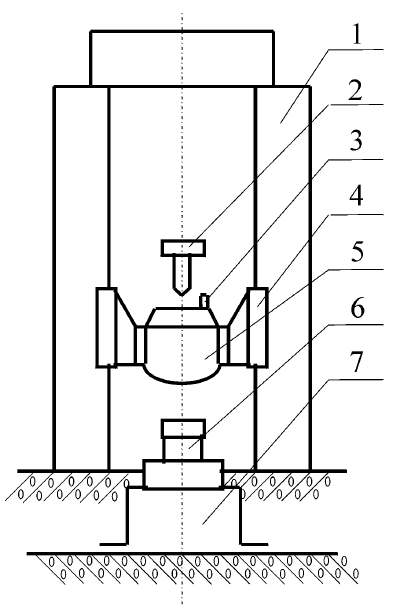
\includegraphics[width=4cm]{cn_100t.png} \\
    1.立柱 2.提升释放机构 3.标准冲击加速度计 \\
    4.导轨 5.重锤 6.被校力传感器 7.底座 \\
  \bicaption[出现在插图索引中]
    {单个图形示例\cite{He1999}。如果表格的标题很长,那么在表格索引中就会很不美观。可
      以在前面用中括号写一个简短的标题,这个标题会出现在索引中。}
    {Stay hungry, stay foolish.}
 \label{fig:cn_100t}
\end{figure}

Lorem ipsum dolor sit amet, consectetur adipisici elit, sed do eiusmod tempor
incididunt ut labore et dolore magna aliqua. Ut enim ad minim veniam, quis
nostrud exercitation ullamco laboris nisi ut aliquip ex ea commodo consequat.
Duis aute irure dolor in reprehenderit in voluptate velit esse cillum dolore eu
fugiat nulla pariatur. Excepteur sint occaecat cupidatat non proident, sunt in
culpa qui officia deserunt mollit anim id est laborum.

\subsection{多个图形}

简单插入多个图形的例子如图~\ref{fig:SRR} 所示。这两个水平并列放置的子图共用一个
图形计数器,没有各自的子图题。

\begin{figure}[!htp]
  \centering
  
\includegraphics[height=2cm]{sjtu-vi-badge-blue.pdf}
  \hspace{1cm}
  
\includegraphics[height=2cm]{sjtu-vi-badge-blue.pdf}
  \bicaption{中文题图}{English caption}
  \label{fig:SRR}
\end{figure}

如果多个图形相互独立,并不共用一个图形计数器,那么用 \texttt{minipage} 或者
\texttt{parbox} 就可以,如图~\ref{fig:parallel1} 与图~\ref{fig:parallel2}。

\begin{figure}[!htp]
\begin{minipage}{0.48\textwidth}
  \centering
  
\includegraphics[height=1.5cm]{sjtu-vi-name-blue.pdf}
  \caption{并排第一个图}
  \label{fig:parallel1}
\end{minipage}\hfill
\begin{minipage}{0.48\textwidth}
  \centering
  
\includegraphics[height=1.5cm]{sjtu-vi-name-blue.pdf}
  \caption{并排第二个图}
  \label{fig:parallel2}
\end{minipage}
\end{figure}

Lorem ipsum dolor sit amet, consectetur adipisici elit, sed do eiusmod tempor
incididunt ut labore et dolore magna aliqua. Ut enim ad minim veniam, quis
nostrud exercitation ullamco laboris nisi ut aliquip ex ea commodo consequat.
Duis aute irure dolor in reprehenderit in voluptate velit esse cillum dolore eu
fugiat nulla pariatur. Excepteur sint occaecat cupidatat non proident, sunt in
culpa qui officia deserunt mollit anim id est laborum.

如果要为共用一个计数器的多个子图添加子图题,建议使用较新的 \pkg{subcaption}宏
包,不建议使用 \pkg{subfigure} 或 \pkg{subfig} 等宏包。

推荐使用 \pkg{subcaption} 宏包的 \cs{subcaptionbox} 并排子图,子图题置于子图之
下,子图号用 a)、b) 等表示。也可以使用 \pkg{subcaption} 宏包的 \cs{subcaption}
(放在 minipage中,用法同 \cs{caption})。

搭配 \pkg{bicaption} 宏包时,可以启用 \cs{subcaptionbox} 和 \cs{subcaption} 的双
语变种 \cs{bisubcaptionbox} 和 \cs{bisubcaption},如图~\ref{fig:bisubcaptionbox}
所示。

\begin{figure}[!hbtp]
  \centering
  \bisubcaptionbox{$R_3 = 1.5\text{mm}$ 时轴承的压力分布云图}%
                  {Pressure contour of bearing when $R_3 = 1.5\text{mm}$}%
                  [6.4cm]{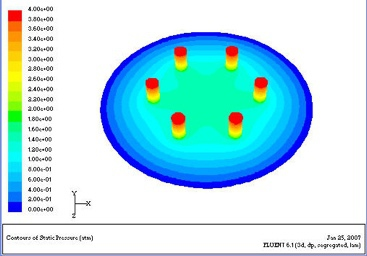
\includegraphics[height=2.5cm]{pressure15.jpg}}
  \hspace{1cm}
  \bisubcaptionbox{$R_3 = 2.5\text{mm}$ 时轴承的压力分布云图}%
                  {Pressure contour of bearing when $R_3 = 2.5\text{mm}$}%
                  [6.4cm]{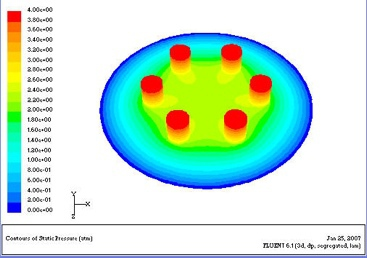
\includegraphics[height=2.5cm]{/pressure25.jpg}}
  \bicaption{包含子图题的范例(使用 subcaptionbox)}
            {Example with subcaptionbox}
  \label{fig:bisubcaptionbox}
\end{figure}

\pkg{subcaption} 宏包也提供了 \pkg{subfigure} 和 \pkg{subtable} 环境,如
图~\ref{fig:subfigure}。

\begin{figure}[!htp]
  \centering
  \begin{subfigure}{0.3\textwidth}
    \centering
    
\includegraphics[height=2cm]{sjtu-vi-badge-blue.pdf}
    \caption{校徽}
  \end{subfigure}
  \hspace{1cm}
  \begin{subfigure}{0.4\textwidth}
    \centering
    
\includegraphics[height=1.5cm]{sjtu-vi-name-blue.pdf}
    \caption{校名。注意这个图略矮些,subfigure 中同一行的子图在顶端对齐。}
  \end{subfigure}
  \caption{包含子图题的范例(使用 subfigure)}
  \label{fig:subfigure}
\end{figure}

Lorem ipsum dolor sit amet, consectetur adipisici elit, sed do eiusmod tempor
incididunt ut labore et dolore magna aliqua. Ut enim ad minim veniam, quis
nostrud exercitation ullamco laboris nisi ut aliquip ex ea commodo consequat.
Duis aute irure dolor in reprehenderit in voluptate velit esse cillum dolore eu
fugiat nulla pariatur. Excepteur sint occaecat cupidatat non proident, sunt in
culpa qui officia deserunt mollit anim id est laborum.

\section{表格}

\subsection{基本表格}

编排表格应简单明了,表达一致,明晰易懂,表文呼应、内容一致。表题置于表上,研究生
学位论文可以用中、英文两种文字居中排写,中文在上,也可以只用中文。

表格的编排建议采用国际通行的三线表\footnote{三线表,以其形式简洁、功能分明、阅读
方便而在科技论文中被推荐使用。三线表通常只有 3 条线,即顶线、底线和栏目线,没有
竖线。}。三线表可以使用 \pkg{booktabs} 提供的 \cs{toprule}、\cs{midrule} 和
\cs{bottomrule}。它们与 \pkg{longtable} 能很好的配合使用。

\begin{table}[!hpt]
  \caption[一个颇为标准的三线表]{一个颇为标准的三线表\footnotemark}
  \label{tab:firstone}
  \centering
  \begin{tabular}{@{}llr@{}} \toprule
    \multicolumn{2}{c}{Item} \\ \cmidrule(r){1-2}
    Animal & Description & Price (\$)\\ \midrule
    Gnat  & per gram  & 13.65 \\
          & each      & 0.01 \\
    Gnu   & stuffed   & 92.50 \\
    Emu   & stuffed   & 33.33 \\
    Armadillo & frozen & 8.99 \\ \bottomrule
  \end{tabular}
\end{table}
\footnotetext{这个例子来自
  \href{https://mirrors.sjtug.sjtu.edu.cn/ctan/macros/latex/contrib/booktabs/booktabs.pdf}%
  {《Publication quality tables in LaTeX》}(\pkg{booktabs} 宏包的文档)。这也是
  一个在表格中使用脚注的例子,请留意与 \pkg{threeparttable} 实现的效果有何不
  同。}

\subsection{复杂表格}

我们经常会在表格下方标注数据来源,或者对表格里面的条目进行解释。可以用
\pkg{threeparttable} 实现带有脚注的表格,如表~\ref{tab:footnote}。

\begin{table}[!htpb]
  \bicaption{一个带有脚注的表格的例子}{A Table with footnotes}
  \label{tab:footnote}
  \centering
  \begin{threeparttable}[b]
     \begin{tabular}{ccd{4}cccc}
      \toprule
      \multirow{2}*{total} & \multicolumn{2}{c}{20\tnote{a}} & \multicolumn{2}{c}{40} & \multicolumn{2}{c}{60} \\
      \cmidrule(lr){2-3}\cmidrule(lr){4-5}\cmidrule(lr){6-7}
      & www & \multicolumn{1}{c}{k} & www & k & www & k \\ % 使用说明符 d 的列会自动进入数学模式,使用 \multicolumn 对文字表头做特殊处理
      \midrule
      & $\underset{(2.12)}{4.22}$ & 120.0140\tnote{b} & 333.15 & 0.0411 & 444.99 & 0.1387 \\
      & 168.6123 & 10.86 & 255.37 & 0.0353 & 376.14 & 0.1058 \\
      & 6.761    & 0.007 & 235.37 & 0.0267 & 348.66 & 0.1010 \\
      \bottomrule
    \end{tabular}
    \begin{tablenotes}
    \item [a] the first note.% or \item [a]
    \item [b] the second note.% or \item [b]
    \end{tablenotes}
  \end{threeparttable}
\end{table}

Lorem ipsum dolor sit amet, consectetur adipisici elit, sed do eiusmod tempor
incididunt ut labore et dolore magna aliqua. Ut enim ad minim veniam, quis
nostrud exercitation ullamco laboris nisi ut aliquip ex ea commodo consequat.
Duis aute irure dolor in reprehenderit in voluptate velit esse cillum dolore eu
fugiat nulla pariatur. Excepteur sint occaecat cupidatat non proident, sunt in
culpa qui officia deserunt mollit anim id est laborum.

如某个表需要转页接排,可以用 \pkg{longtable} 实现。接排时表题省略,表头应重复书
写,并在右上方写“续表 xx”,如表~\ref{tab:performance}。

\begin{ThreePartTable}
  \begin{TableNotes}
    \item[a] 一个脚注
    \item[b] 另一个脚注
  \end{TableNotes}
  \begin{longtable}[c]{c*{6}{r}}
    \bicaption{实验数据}{Experimental data}
    \label{tab:performance} \\
    \toprule
    测试程序 & \multicolumn{1}{c}{正常运行} & \multicolumn{1}{c}{同步}
      & \multicolumn{1}{c}{检查点} & \multicolumn{1}{c}{卷回恢复}
      & \multicolumn{1}{c}{进程迁移} & \multicolumn{1}{c}{检查点} \\
    & \multicolumn{1}{c}{时间 (s)} & \multicolumn{1}{c}{时间 (s)}
      & \multicolumn{1}{c}{时间 (s)} & \multicolumn{1}{c}{时间 (s)}
      & \multicolumn{1}{c}{时间 (s)} &  文件(KB)\\
    \midrule
    \endfirsthead
    \multicolumn{7}{r}{续表~\thetable} \\
    \toprule
    测试程序 & \multicolumn{1}{c}{正常运行} & \multicolumn{1}{c}{同步}
      & \multicolumn{1}{c}{检查点} & \multicolumn{1}{c}{卷回恢复}
      & \multicolumn{1}{c}{进程迁移} & \multicolumn{1}{c}{检查点} \\
    & \multicolumn{1}{c}{时间 (s)} & \multicolumn{1}{c}{时间 (s)}
      & \multicolumn{1}{c}{时间 (s)} & \multicolumn{1}{c}{时间 (s)}
      & \multicolumn{1}{c}{时间 (s)}&  文件(KB)\\
    \midrule
    \endhead
    \hline
    \multicolumn{7}{r}{续下页}
    \endfoot
    \insertTableNotes
    \endlastfoot
    CG.A.2 & 23.05 & 0.002 & 0.116 & 0.035 & 0.589 & 32491 \\
    CG.A.4 & 15.06 & 0.003 & 0.067 & 0.021 & 0.351 & 18211 \\
    CG.A.8 & 13.38 & 0.004 & 0.072 & 0.023 & 0.210 & 9890 \\
    CG.B.2 & 867.45 & 0.002 & 0.864 & 0.232 & 3.256 & 228562 \\
    CG.B.4 & 501.61 & 0.003 & 0.438 & 0.136 & 2.075 & 123862 \\
    CG.B.8 & 384.65 & 0.004 & 0.457 & 0.108 & 1.235 & 63777 \\
    MG.A.2 & 112.27 & 0.002 & 0.846 & 0.237 & 3.930 & 236473 \\
    MG.A.4 & 59.84 & 0.003 & 0.442 & 0.128 & 2.070 & 123875 \\
    MG.A.8 & 31.38 & 0.003 & 0.476 & 0.114 & 1.041 & 60627 \\
    MG.B.2 & 526.28 & 0.002 & 0.821 & 0.238 & 4.176 & 236635 \\
    MG.B.4 & 280.11 & 0.003 & 0.432 & 0.130 & 1.706 & 123793 \\
    MG.B.8 & 148.29 & 0.003 & 0.442 & 0.116 & 0.893 & 60600 \\
    LU.A.2 & 2116.54 & 0.002 & 0.110 & 0.030 & 0.532 & 28754 \\
    LU.A.4 & 1102.50 & 0.002 & 0.069 & 0.017 & 0.255 & 14915 \\
    LU.A.8 & 574.47 & 0.003 & 0.067 & 0.016 & 0.192 & 8655 \\
    LU.B.2 & 9712.87 & 0.002 & 0.357 & 0.104 & 1.734 & 101975 \\
    LU.B.4 & 4757.80 & 0.003 & 0.190 & 0.056 & 0.808 & 53522 \\
    LU.B.8 & 2444.05 & 0.004 & 0.222 & 0.057 & 0.548 & 30134 \\
    EP.A.2 & 123.81 & 0.002 & 0.010 & 0.003 & 0.074 & 1834 \\
    EP.A.4 & 61.92 & 0.003 & 0.011 & 0.004 & 0.073 & 1743 \\
    EP.A.8 & 31.06 & 0.004 & 0.017 & 0.005 & 0.073 & 1661 \\
    EP.B.2 & 495.49 & 0.001 & 0.009 & 0.003 & 0.196 & 2011 \\
    EP.B.4 & 247.69 & 0.002 & 0.012 & 0.004 & 0.122 & 1663 \\
    EP.B.8 & 126.74 & 0.003 & 0.017 & 0.005 & 0.083 & 1656 \\
    SP.A.2 & 123.81 & 0.002 & 0.010 & 0.003 & 0.074 & 1854 \\
    SP.A.4 & 51.92 & 0.003 & 0.011 & 0.004 & 0.073 & 1543 \\
    SP.A.8 & 31.06 & 0.004 & 0.017 & 0.005 & 0.073 & 1671 \\
    SP.B.2 & 495.49 & 0.001 & 0.009 & 0.003 & 0.196 & 2411 \\
    SP.B.4 \tnote{a} & 247.69 & 0.002 & 0.014 & 0.006 & 0.152 & 2653 \\
    SP.B.8 \tnote{b} & 126.74 & 0.003 & 0.017 & 0.005 & 0.082 & 1755 \\
    \bottomrule
  \end{longtable}
\end{ThreePartTable}

\section{算法环境}

算法环境可以使用 \pkg{algorithms} 宏包或者较新的 \pkg{algorithm2e} 实现。
算法~\ref{algo:algorithm} 是一个使用 \pkg{algorithm2e} 的例子。关于排版算法环境
的具体方法,请阅读相关宏包的官方文档。

\begin{algorithm}[htb]
  \caption{算法示例}
  \label{algo:algorithm}
  \small
  \SetAlgoLined
  \KwData{this text}
  \KwResult{how to write algorithm with \LaTeXe }

  initialization\;
  \While{not at end of this document}{
    read current\;
    \eIf{understand}{
      go to next section\;
      current section becomes this one\;
    }{
      go back to the beginning of current section\;
    }
  }
\end{algorithm}

\section{代码环境}

我们可以在论文中插入算法,但是不建议插入大段的代码。如果确实需要插入代码,建议使
用 \pkg{listings} 宏包。

\begin{codeblock}[language=C]
#include <stdio.h>
#include <unistd.h>
#include <sys/types.h>
#include <sys/wait.h>

int main() {
  pid_t pid;

  switch ((pid = fork())) {
  case -1:
    printf("fork failed\n");
    break;
  case 0:
    /* child calls exec */
    execl("/bin/ls", "ls", "-l", (char*)0);
    printf("execl failed\n");
    break;
  default:
    /* parent uses wait to suspend execution until child finishes */
    wait((int*)0);
    printf("is completed\n");
    break;
  }

  return 0;
}
\end{codeblock}

%% !TEX root = ../main.tex

\begin{summary}
这里是全文总结内容。

2015 年 2 月 28 日,中央在北京召开全国精神文明建设工作表彰暨学雷锋志愿服务大会,
公布全国文明城市(区)、文明村镇、文明单位名单。上海交通大学荣获全国文明单位称
号。

全国文明单位这一荣誉是对交大人始终高度重视文明文化工作的肯定,是对交大长期以来文
明创建工作成绩的褒奖。在学校党委、文明委的领导下,交大坚持将文明创建工作纳入学校
建设世界一流大学的工作中,全体师生医护员工群策群力、积极开拓,落实国家和上海市有
关文明创建的各项要求,以改革创新、科学发展为主线,以质量提升为目标,聚焦文明创建
工作出现的重点和难点,优化文明创建工作机制,传播学校良好形象,提升社会美誉度,显
著增强学校软实力。2007 至 2012 年间,上海交大连续三届荣获“上海市文明单位”称
号,成为创建全国文明单位的新起点。

上海交大自启动争创全国文明单位工作以来,凝魂聚气、改革创新,积极培育和践行社会主
义核心价值观。坚持统筹兼顾、多措并举,将争创全国文明单位与学校各项中心工作紧密结
合,着力构建学校文明创建新格局,不断提升师生医护员工文明素养,以“冲击世界一流大
学汇聚强大精神动力”为指导思想,以“聚焦改革、多元推进、以评促建、丰富内涵、彰显
特色”为工作原则,并由全体校领导群策领衔“党的建设深化、思想教育深入、办学成绩显
著、大学文化丰富、校园环境优化、社会责任担当”六大板块共 28 项重点突破工作,全面
展现近年来交大文明创建工作的全貌和成就。

进入新阶段,学校将继续开拓文明创建工作新格局,不断深化工作理念和工作实践,创新工
作载体、丰富活动内涵、凸显创建成效,积极服务于学校各项中心工作和改革发展的大局
面,在上级党委、文明委的关心下,在学校党委的直接领导下,与时俱进、开拓创新,为深
化内涵建设、加快建成世界一流大学、推动国家进步和社会发展而努力奋斗!

上海交通大学医学院附属仁济医院也获得全国文明单位称号。
\end{summary}


%TC:ignore

% 参考文献
\printbibliography[heading=bibintoc]

% 附录
%\appendix

% 附录中图表不加入索引
\captionsetup{list=no}

% 附录内容
%% !TEX root = ../main.tex

\chapter{Maxwell Equations}

选择二维情况,有如下的偏振矢量:
\begin{subequations}
  \begin{align}
    {\bf E} &= E_z(r, \theta) \hat{\bf z}, \\
    {\bf H} &= H_r(r, \theta) \hat{\bf r} + H_\theta(r, \theta) \hat{\bm\theta}.
  \end{align}
\end{subequations}
对上式求旋度:
\begin{subequations}
  \begin{align}
    \nabla \times {\bf E} &= \frac{1}{r} \frac{\partial E_z}{\partial\theta}
      \hat{\bf r} - \frac{\partial E_z}{\partial r} \hat{\bm\theta}, \\
    \nabla \times {\bf H} &= \left[\frac{1}{r} \frac{\partial}{\partial r}
      (r H_\theta) - \frac{1}{r} \frac{\partial H_r}{\partial\theta} \right]
      \hat{\bf z}.
  \end{align}
\end{subequations}
因为在柱坐标系下,$\overline{\overline\mu}$ 是对角的,所以 Maxwell 方程组中电场
$\bf E$ 的旋度:
\begin{subequations}
  \begin{align}
    & \nabla \times {\bf E} = \ii \omega {\bf B}, \\
    & \frac{1}{r} \frac{\partial E_z}{\partial\theta} \hat{\bf r} -
      \frac{\partial E_z}{\partial r}\hat{\bm\theta} = \ii \omega \mu_r H_r
      \hat{\bf r} + \ii \omega \mu_\theta H_\theta \hat{\bm\theta}.
  \end{align}
\end{subequations}
所以 $\bf H$ 的各个分量可以写为:
\begin{subequations}
  \begin{align}
    H_r &= \frac{1}{\ii \omega \mu_r} \frac{1}{r}
      \frac{\partial E_z}{\partial\theta}, \\
    H_\theta &= -\frac{1}{\ii \omega \mu_\theta}
      \frac{\partial E_z}{\partial r}.
  \end{align}
\end{subequations}
同样地,在柱坐标系下,$\overline{\overline\epsilon}$ 是对角的,所以 Maxwell 方程
组中磁场 $\bf H$ 的旋度:
\begin{subequations}
  \begin{align}
    & \nabla \times {\bf H} = -\ii \omega {\bf D}, \\
    & \left[\frac{1}{r} \frac{\partial}{\partial r}(r H_\theta) - \frac{1}{r}
      \frac{\partial H_r}{\partial\theta} \right] \hat{\bf z} = -\ii \omega
      {\overline{\overline\epsilon}} {\bf E} = -\ii \omega \epsilon_z E_z
      \hat{\bf z}, \\
    & \frac{1}{r} \frac{\partial}{\partial r}(r H_\theta) - \frac{1}{r}
      \frac{\partial H_r}{\partial\theta} = -\ii \omega \epsilon_z E_z.
  \end{align}
\end{subequations}
由此我们可以得到关于 $E_z$ 的波函数方程:
\begin{equation}
  \frac{1}{\mu_\theta \epsilon_z} \frac{1}{r} \frac{\partial}{\partial r}
  \left(r \frac{\partial E_z}{\partial r} \right) + \frac{1}{\mu_r \epsilon_z}
  \frac{1}{r^2} \frac{\partial^2E_z}{\partial\theta^2} +\omega^2 E_z = 0.
\end{equation}

%% !TEX root = ../main.tex

\chapter{绘制流程图}

图~\ref{fig:flow_chart} 是一张流程图示意。使用 \pkg{tikz} 环境,搭配四种预定义节
点(\verb+startstop+、\verb+process+、\verb+decision+和\verb+io+),可以容易地绘
制出流程图。

\begin{figure}[!htp]
  \centering
  \resizebox{6cm}{!}{
% 定义流程图节点
\tikzstyle{startstop} = [
  rectangle,
  rounded corners,
  minimum width=2cm,
  minimum height=1cm,
  text centered,
  draw=black
]
\tikzstyle{io} = [
  trapezium,
  trapezium left angle=75,
  trapezium right angle=105,
  minimum width=1cm,
  minimum height=1cm,
  text centered,
  draw=black
]
\tikzstyle{process} = [
  rectangle,
  minimum width=2cm,
  minimum height=1cm,
  text centered,
  draw=black
]
\tikzstyle{decision} = [
  diamond,
  minimum width=2cm,
  minimum height=1cm,
  text centered,
  draw=black]
\tikzstyle{arrow} = [thick, ->, >=stealth]

\begin{tikzpicture}[node distance=2cm]
  % 设置节点
  \node (pic) [startstop] {待测图片};
  \node (bg) [io, below of=pic] {读取背景};
  \node (pair) [process, below of=bg] {匹配特征点对};
  \node (threshold) [decision, below of=pair, yshift=-0.5cm] {多于阈值};
  \node (clear) [decision, right of=threshold, xshift=3cm] {清晰?};
  \node (capture) [process, right of=pair, xshift=3cm, yshift=0.5cm] {重采};
  \node (matrix_p) [process, below of=threshold, yshift=-0.8cm] {透视变换矩阵};
  \node (matrix_a) [process, right of=matrix_p, xshift=3cm] {仿射变换矩阵};
  \node (reg) [process, below of=matrix_p] {图像修正};
  \node (return) [startstop, below of=reg] {配准结果};
    
  % 连接节点
  \draw [arrow](pic) -- (bg);
  \draw [arrow](bg) -- (pair);
  \draw [arrow](pair) -- (threshold);

  \draw [arrow](threshold) -- node[anchor=south] {否} (clear);

  \draw [arrow](clear) -- node[anchor=west] {否} (capture);
  \draw [arrow](capture) |- (pic);
  \draw [arrow](clear) -- node[anchor=west] {是} (matrix_a);
  \draw [arrow](matrix_a) |- (reg);

  \draw [arrow](threshold) -- node[anchor=east] {是} (matrix_p);
  \draw [arrow](matrix_p) -- (reg);
  \draw [arrow](reg) -- (return);
\end{tikzpicture}
}
  \bicaption{绘制流程图效果}{Flow chart}
  \label{fig:flow_chart}
\end{figure}


% 结尾部分
\backmatter

% 用于盲审的论文需隐去致谢、发表论文、科研成果、简历

% 致谢
%% !TEX root = ../main.tex

\begin{acknowledgements}

大学生活步入尾声,在完成毕业设计的过程中我收获良多。首先要感谢我的毕业设计指导老师邹福泰老师,邹老师在毕设期间定期每周召开组会,与我们交流指导,督促我们的进展,为我们的工作提出了许多宝贵的意见。


感谢邹老师鼓励我参加了第三十四届全国大学生信息安全竞赛。在整个备赛过程中,邹老师全程与我们保持密切联系,悉心指导我们的工作,老师对最终论文格式要求严格而缜密,令我印象深刻,最终我们团队取得了二等奖的满意成绩。由于我参与了竞赛课题的大部分工作,收获颇丰,包括了机器学习、挖矿脚本、挂马网站等培养计划中没有深入涉及的有趣知识。邹老师为人随和,指导学生富有耐心,令我懂得在课题中面对各种棘手的方法也要放平心态,时间紧张的情况下也要井井有条。再次感谢邹老师在科研方面对我的鼓励与指导。


其次,我想感谢向立瑶老师对我的帮助。在PRP期间我参加了向立瑶老师的课题小组,组内同学科研水平高、代码能力强,每周一次的组会讨论内容详细、信息量丰富。在此期间,我认识到了科研论文发表所需要的大量的准备工作,我的科研文献阅读能力有了很大提升,对机器学习也有了更加深入的了解,极大拓宽了我的眼界。


感谢我的同学贺皓涵。在大三期间贺皓涵同学与我都面临竞赛、PRP以及较为繁重的课业多项任务重叠的期间,我们互相支持、互帮互助,渡过了那段繁忙的时光。感谢我的好友吴进华和金益彰,大学最快乐的时光总有他们的陪伴。


最后,感谢父母长期以来的无私付出,家人的鼓励是我克服困难、专注学业的基础,回报父母将成为我未来道路中的一大动力。大学生活即将结束,今后的人生充满可能性,愿自己脚踏实地,为了理想和目标而不停奋斗。

\end{acknowledgements}


% 发表论文及科研成果
% 盲审论文中,发表论文及科研成果等仅以第几作者注明即可,不要出现作者或他人姓名
%% !TEX root = ../main.tex

\begin{achievements}

\subsection*{学术论文}

\begin{bibliolist}{00}
  \item Chen H, Chan C~T. Acoustic cloaking in three dimensions using acoustic metamaterials[J]. Applied Physics Letters, 2007, 91:183518.
  \item Chen H, Wu B~I, Zhang B, et al. Electromagnetic Wave Interactions with a Metamaterial Cloak[J]. Physical Review Letters, 2007, 99(6):63903.
\end{bibliolist}

\begin{bibliolist*}{00}
  \item 第一作者. 中文核心期刊论文, 2007.
  \item 第一作者. EI 国际会议论文, 2006.
\end{bibliolist*}

\subsection*{专利}

\begin{bibliolist}{00}
  \item 第一发明人,“永动机”,专利申请号202510149890.0
\end{bibliolist}

\begin{bibliolist*}{00}
  \item 第一发明人,“永动机”,专利申请号XXXXXXXXXXXX.X
\end{bibliolist*}

\end{achievements}


% 简历
%% !TEX root = ../main.tex

\begin{resume}
  \subsection*{基本情况}
    某某,yyyy 年 mm 月生于 xxxx。

  \subsection*{教育背景}
  \begin{itemize}
    \item yyyy 年 mm 月至今,上海交通大学,博士研究生,xx 专业
    \item yyyy 年 mm 月至 yyyy 年 mm 月,上海交通大学,硕士研究生,xx 专业
    \item yyyy 年 mm 月至 yyyy 年 mm 月,上海交通大学,本科,xx 专业
  \end{itemize}

  \subsection*{研究兴趣}
    \LaTeX{} 排版

  \subsection*{联系方式}
  \begin{itemize}
    \item 地址: 上海市闵行区东川路 800 号,200240
    \item E-mail: \email{xxx@sjtu.edu.cn}
  \end{itemize}
\end{resume}


% 学士学位论文要求在最后有一个大摘要,单独编页码
%% !TEX root = ../main.tex

\begin{digest}
With the rapid development of new technologies such as containers and micro services, open source software has become the mainstream in the industry, and the software industry has developed rapidly

Exhibition. Most modern software is "assembled" rather than "developed". According to Forrester statistics, 80-90\% of the code in software development comes from open source software \cite{qianxin.com}. Therefore, the source code of modern software is mostly mixed source code, which is composed of source code independently developed by enterprises and open source software code. Appbrain \cite{appbrain} tracked 450 popular libraries, and the statistical results show that they are in the Android ecosystem

Mobile phone library is especially popular in the network and analysis system. Such extensive use of third-party libraries not only accelerates the development process and avoids repeated wheel building, but also attracts attackers to move their targets upstream of the software supply chain to attack applications by exploiting the vulnerabilities of popular libraries. Therefore, the detection of third-party database has become an urgent problem to be solved. The existing research methods can be divided into two categories: prior knowledge and no prior knowledge. The former needs the help of the standard third-party open source warehouse to achieve the detection goal through the extraction and matching of various features of the third-party library and the standard library in the app. The latter does not need external knowledge. Starting from the large-scale app data set and based on the clustering algorithm, the modules with class inheritance, function call and other connections are gathered together as the candidate database. When enough candidates appear and their similarity is high, they are considered to be from a third-party database. With the development of obfuscation technology, anti-obfuscation on has become a point that can not be ignored in research methods. Name based technology has been difficult to achieve satisfactory performance. In addition, the current research work on the detection of specific versions of third-party libraries is not much, and there are still some problems, such as how to accurately represent version differences and how to deal with large-scale data sets caused by a large number of versions.



Based on the above background, this paper proposes an Android application third-party library detection system TPL-V Detector based on a priori knowledge, which can resist obfuscation and be accurate to the specific version. In the system design, this paper first introduces the APK, jar and other files as the system input, as well as the DEX, class and bytecode files involved in the preprocessing process. Taking bytecode file as the input after processing, TPL-V Detector constructs a feature tree in the unit of package, and organizes all kinds of methods under the package and classes in the tree structure. Further, TPL-V Detector extracts the coarse-grained features based on function descriptors and the fine-grained features based on bytecode instruction sequences from bytecode files, calculates their hash values as the features of the method, and generates the features of classes according to the tree structure. The characteristics of the class are used to match the package. According to the similarity calculation method used in this paper, the package exceeding the threshold is regarded as the third-party library used in the detected app. The specific design details of TPL-V Detector are as follows.



TPL-V Detector can be divided into four modules: preprocessing, building feature tree, feature storage and feature matching. In the preprocessing module, APK and jar files are decompressed to obtain class files. Each class file corresponds to a class. Class file is further converted into bytecode file, which contains function descriptor, bytecode instruction sequence, constant pool and so on. In order to prevent obfuscation operations from changing the name, the return value name and parameter name in the function descriptor are deleted, only their types are retained, and the MD5 hash value of this string is calculated as the coarse-grained feature of the method. Due to the stack based nature of Java, bytecode instructions are operations on the stack and do not contain string classes. Therefore, connect the instruction sequences of a method and calculate the MD5 hash value as its fine-grained feature. Each path that contains a class file and its upper folder does not contain a class file is regarded as the root directory of a package, and a feature tree is constructed according to this directory and its contents. The root package is the root node of the tree, each type is the child node of the root, and each method under the class is the leaf node of this type of node. According to the tree structure, the features of the method are used to generate the features of the class. The specific method is to arrange and connect the features of the method according to the dictionary order, and calculate its fuzzy hash value as the result. For libraries from Maven central warehouse \cite{maven}, TPL-V Detector calculates their characteristics according to the above method and stores them in MySQL database. Each line records key information such as package name, class name, method name, characteristics of class and method. Records from Maven belong to the same design pattern as those from app and are stored in different tables under the same database. In the feature matching module, TPL-V Detector first uses coarse-grained features to select the class of the standard library with the highest similarity to its features in the database for each class in the app as its best match. The sum of the similarity of various best matches multiplied by the weight of the methods contained in them is the similarity score of the package. Packages that exceed the predefined threshold are regarded as a matching result of the current app package. After the package used by the app is detected, the fine-grained feature is further used to match versions within different versions of the package in the same way. In addition to the two-level feature strategy, based on the assumption that most classes belonging to the same package are placed in the same folder, TPL-V Detector also introduces the strategy of priority queue, which puts several best matching results of the class to be matched in the current app into the priority queue. When the class to be matched arrives, it is likely to find a match with high similarity in the priority queue.



Multiple experiments were conducted to detect the performance of TPL-V Detector. Firstly, experiments were carried out on the standard third-party database dataset from Maven. For the six selected libraries and their different versions, the experiment used Proguard to confuse them. The matching similarity of the best results of TPL-V Detector on each library can reach more than 0.8, which is much higher than the non best results, indicating that TPL-V Detector has excellent feature extraction and processing ability, and can easily distinguish different libraries even in the case of obfuscation. Then, the detection performance is evaluated on the actual android app. Firstly, the best experimental parameters are selected by depicting the change curve of each index with the threshold. For the 10 selected apps and the 9 third-party libraries used therein, TPL-V Detector detected most of them, and only performed poorly in individual libraries with a very large number of versions, reaching an accuracy rate of 88.0\% and a recall rate of 81.5\%. The experiment then discusses TPL-V Detector in detail. Firstly, the time cost of its four stages is evaluated. The construction of feature tree and feature generation take less time. In app preprocessing stage, due to the need to call third-party programs many times, it reaches 60\% to 70\% of the total time cost. In addition, the experiment also discusses the optimization effect of two-level feature and priority queue matching strategies. The time optimization of two-level feature on feature matching stage is very obvious. According to the size of database, the time can be shortened to 1/2 to 1/5 without any strategy. Priority queue can further optimize the time overhead on the premise of applying two-level characteristic strategy. Finally, the comparative experiment between TPL-V Detector and existing tools is carried out. Combined with the indicators of accuracy, recall and F1 score, TPL-V Detector has achieved the best performance.



In general, the contributions of this paper are as follows.(1) This paper proposes TPL-V Detector, a third-party library detection system, which can not only accurately identify the third-party library, but also accurate to the specific version. (2) This paper proposes a feature generation method based on descriptor type and bytecode instruction sequence, which makes TPL-V Detector still have a good performance in detecting confused apps. (3) This paper introduces the coarse / fine-grained features, and adds the priority queue strategy in the process of database matching, which effectively optimizes the simple matching method and saves time. (4) This paper evaluates on Maven data set, which can accurately match the SDK before and after obfuscation one by one, and achieve 100\% accuracy under the invitation of more than 200 versions in 6 libraries. (5) In this paper, the experimental test is carried out with the self built app data set, and the time overhead in different stages is analyzed in detail. Considering many factors such as version recognition and accuracy, it has good performance, and the accuracy is as high as 98\%.



To sum up, this paper proposes an Android application third-party library and its version detection system based on a priori knowledge and anti-obfuscation, which has achieved good performance in the experimental evaluation and achieved the expected research goal of the subject.

\end{digest}


%TC:endignore

\end{document}
